%%%%%%%%%%%%%%%%%%%%%%%%%%%%%%%%%%%%%%%%%%%%%%%%%%%%%%%%%%%%%%%%%%%%%%%%%%%%%
%%                                                                         %%
%%                   LaTeX Vorlage für die Studenten der                   %%
%%              Dualen Hochschule Baden-Württemberg Ravensburg             %%
%%                                                                         %%
%%  Die Vorlage orientiert sich an den Gestaltungsrichtlinien der DHBW RV  %%
%%                                                                         %%
%%                                                                         %%
%% Ersteller:        Markus Schutz (WI06)                                  %%
%% letzten Änderung: 26. November 2013                                     %%
%%                                                                         %%
%%                                                                         %%
%% Wichtiger Hinweis zur Verwendung dieser Vorlage:                        %%
%%                                                                         %%
%% Damit die Vorlage verwendet und die PDF richtig und vollständig erzeugt %%
%% werden kann bedarf des manuellen Aufrufs von makeindex. Diese können    %%
%% optional auch direkt im Editor eingerichtet werden.                     %%
%% TeXnicCenter (Ausgabe -> Ausgabeprofile definieren... (Alt + F7)        %%
%%               LaTeX => PDF -> Nachbearbeitung)                          %%
%%                                                                         %%
%% (1) Stichwortverzeichnis (falls verwendet)                              %%
%% makeindex -g -s styles\stichwortverzeichnis.ist vorlage                 %%
%% (2) Abkürzungsverzeichnis                                               %%
%% makeindex vorlage.nlo -s nomencl.ist -o vorlage.nls                     %%
%% (3) Glossar (falls verwendet)                                           %%
%% makeindex -s vorlage.ist -t vorlage.glg -o vorlage.gls vorlage.glo      %%
%% 
%% In Texstudio: txs:///makeindex "%.idx" -t "%.ilg" -o "%.ind" | txs:///makeindex -g -s "styles/stichwortverzeichnis.ist" % | txs:///makeindex "%.nlo" -s nomencl.ist -o "%.nls"
%% Als eigenen Befehl "alles" eintragen									   %%
%% Dann Reihenfolge: PdfLatex, Bibtex, alles, Pdflatex, Pdflatex		   %%
%%                                                                         %%
%% Bei der Erzeugung der PDF Datei (Anwendung des LaTeX => PDF Ausgabe-    %%
%% profiles) werden das Abkürzungsverzeichnis, das Stichwortverzeichnis    %%
%% und das Glossar jetzt richtig erzeugt. In Verbindung mit TeXnicCenter   %%
%% kann es beim automatisierten Aufruf von makeindex zu Probleme kommen.   %%
%% Ein manueller Aufruf funktioniert dagegen immer.                        %%
%%                                                                         %%
%% Wichtiger Hinweis:                                                      %%
%%                                                                         %%
%% Keine Änderungen an den Dateien im Verzeichnis "pages" vornehmen. Für   %%
%% die Arbeit beziehen sich alle Änderungen auf diese Datei und die        %%
%% Dateien im Verzeichnis "chapter".                                       %%
%% Für die Erstellung des Literaturverzeichnises empfiehlt sich die Ver-   %%
%% wendung von JabRef (http://jabref.sourceforge.net). Die Datei ist unter %%
%% dem Namen literatur.bib im Verzeichnis "literatur" zu speichern.        %%
%%                                                                         %%
%% Zur sinnvollen Nutzung dieser Vorlage empfiehlt es sich, die Dokus zu   %%
%% den eingebundenen Paketen durchzulesen. Sie sind im doc-Verzeichnis der %%
%% MiKTeX-Installation zu finden.                                          %%
%%                                                                         %%
%% Enthaltene Titelblätter:                                                %%
%%   - Seminararbeit                                                       %%
%%   - Projektarbeit                                                       %%
%%   - Bachelorarbeit                                                      %%
%%                                                                         %%
%%%%%%%%%%%%%%%%%%%%%%%%%%%%%%%%%%%%%%%%%%%%%%%%%%%%%%%%%%%%%%%%%%%%%%%%%%%%%

\documentclass[a4paper,12pt]{article}                                         % Schriftgröße, Layout, Papierformat, Art des Dokumentes
\usepackage[left=3cm,right=2cm,top=2cm,bottom=2cm,includehead]{geometry}      % Einstellungen der Seitenränder
\usepackage[english, ngerman]{babel}                                                   % deutsche Silbentrennung
\usepackage[utf8]{inputenc}                                                   % Umlaute
\usepackage[T1]{fontenc}													  % Umlaute auch richtig ausgeben
\usepackage[hyperfootnotes=false]{hyperref}                                   % pfd-Output [Fußnoten nicht verlinken]
\usepackage[nottoc]{tocbibind}                                                % Inhaltsverzeichniserweiterung (Inhaltsverzeichnis selbst ausblenden)
\usepackage{makeidx}                                                          % Index
\usepackage[intoc]{nomencl}                                                   % Abkürzungsverzeichnis
\usepackage{fancyhdr}                                                         % Fancy Header
\usepackage[round]{natbib}                                                    % Zitate (Erweiterung für Literaturverzeichnis)
\usepackage{amsmath}                                                          % Zurücksetzen der Tabellen- und Abbildungsnummerierung je Sektion
\usepackage[labelfont=bf,aboveskip=1mm]{caption}                              % Bild- und Tabellenunterschrift (fett)
\usepackage[onehalfspacing]{setspace}                                                         % Zeilenabstand (vor footmisc laden!)
\usepackage[bottom,multiple,hang,marginal]{footmisc}                          % Fußnoten [Ausrichtung unten, Trennung durch Seperator bei mehreren Fußnoten]
\usepackage{graphicx}                                                         % Grafiken
\usepackage{tabularx}                                                         % erweiterte Tabellen
\usepackage{longtable}                                                        % mehrseitige Tabellen
\usepackage{color}                                                            % Farben
\usepackage{enumitem}                                                         % Befehl setlist (Zeilenabstand für itemize Umgebung auf 1 setzen)
\usepackage{listings}                                                         % Quelltexte
\usepackage{zref}                                                             % Verweise (Anhangsverweise)
\usepackage[toc,style=altlist,translate=false]{glossaries}                    % Glossar (nach hyperref, inputenc, babel und ngerman)
\usepackage{glossaries-babel}                                                 % Glossar: Übersetzung im TOC
\usepackage{pdfpages}														  % um PDFs einzubinden
\usepackage[gen]{eurosym}													  % für das Eurozeichen. € = \euro{}
\usepackage{here}
\usepackage{float}
\usepackage{svg}
\usepackage{amsmath}
\usepackage{pgfplots}                                                         %allows to create fancy plots directly in latex
\usepackage{ifthen}

%%%%%%%%%%%%%%%%%%%%%%%%%%%%%%%%%%%%%%%%%%%%%%%%%%%%%%%%%%%%%%%%%%%%%%%%%%%%%
%%                                                                         %%
%% \/   \/      Bitte hier die Änderungen zur Arbeit vornehmen     \/   \/ %%
%%                                                                         %%
%%%%%%%%%%%%%%%%%%%%%%%%%%%%%%%%%%%%%%%%%%%%%%%%%%%%%%%%%%%%%%%%%%%%%%%%%%%%%

%%%%%%%%%%%%%%%%%%%%%%% Definitionen bzgl. der Arbeit %%%%%%%%%%%%%%%%%%%%%%%
\def\myType{1}           % [0=Seminararbeit|1=Projektarbeit|2=Bachelorarbeit]

\def\myTopic{KI-gestützte Optimierung von Motorsport - Rennstrategien in einer simulierten Umgebung am Beispiel der Formel 1}
\def\mySubTopic{}
\def\myAutor{Tim Heckenberger && Manuel Kreft && Alexander Müller}
%\def\myAutor{Tim Heckenberger & Manuel Kreft & Alexander Müller}
\def\myCompany{}
\def\myCompanyAddressStreet{}
\def\myCompanyAddressCity{}
\def\myProf{Dipl.-Ing. (BA) Claudia Zinser}
\def\myEndDate{06.2022}
\def\myMatriculationNumber{}
\def\myCourseOfStudies{TIT19}
\def\mySupervisor{}
\def\myProcessingTime{11.2021 - 06.2022}

%%%%%%%%%%%%%%%%%%%% Folgende Angaben für: Seminararbeit %%%%%%%%%%%%%%%%%%%%
\def\myVorlesung{egal}

%%%%%%%%%%%%%%%%%%%% Folgende Angaben für: Projektarbeit %%%%%%%%%%%%%%%%%%%%
\def\myProjNumber{1}         % [1|2]
\def\myPraxPhase{1}                       % [1|2|3]
\def\myPraxYear{erste}         			            % [erste|zweite|dritte]

%%%%%%%%%%%%%%%%%%%%%%%%%%%%%%%%%%%%%%%%%%%%%%%%%%%%%%%%%%%%%%%%%%%%%%%%%%%%%
%%                                                                         %%
%% /\   /\         Ab hier keine Änderungen mehr vornehmen         /\   /\ %%
%%                                                                         %%
%%%%%%%%%%%%%%%%%%%%%%%%%%%%%%%%%%%%%%%%%%%%%%%%%%%%%%%%%%%%%%%%%%%%%%%%%%%%%

%%%%%%%%%%%%%%%%%%%%%%%% Eigene Farbwerte definieren %%%%%%%%%%%%%%%%%%%%%%%%
\definecolor{boxgray}{gray}{0.9}         % Hintergrundfarbe für Zitatboxen
\definecolor{commentgray}{gray}{0.5}     % Grau für Kommentare in Quelltexten
\definecolor{darkgreen}{rgb}{0,.5,0}     % Grün für Strings in Quelltexten



%%%%%%%%%%%%%%%%%%%%%%%% Eigene Kommandos definieren %%%%%%%%%%%%%%%%%%%%%%%%
% Definition von \gqq{#1: text}: Text in Anführungszeichen
\newcommand{\gqq}[1]{\glqq #1\grqq}

% Definition von \footref{#1: label}
% Verweis auf bereits existierende Fußnoten mittels
\providecommand*{\footref}[1]{
	\begingroup
		\unrestored@protected@xdef\@thefnmark{\ref{#1}}
	\endgroup
\@footnotemark}

% Definition von \mypageref{#1: label}
% Kombination aus \ref{#1: label} und \pageref{#1: label}
\newcommand{\mypageref}[1]{\ref{#1} auf Seite \pageref{#1}}

% Definition von \myboxquote{#1: text}
% grau hinterlegte Quotation-Umgebung (für Zitate)
\newcommand{\myboxquote}[1]{
	\begin{quotation}
		\colorbox{boxgray}{\parbox{0.78\textwidth}{#1}}
	\end{quotation}
	\vspace*{1mm}
}

\makeatletter
\zref@newprop*{appsec}{}
\zref@addprop{main}{appsec}

% Definition von \applabel{#1: label}{#2: text}
% von \appsec{#1: text}{#2: label} zur Erzeugung des Labels verwendet)
\def\applabel#1#2{%
	\zref@setcurrent{appsec}{#2}%   
	\zref@wrapper@immediate{\zref@label{#1}}%
}

% Definition von \appref{#1: label}
% anstelle \ref{#1: label} zum referenzieren von Anhängen verwenden)
\def\appref#1{%
	\hyperref[#1]{\zref@extract{#1}{appsec}}%
}
\makeatother

% Definition von \appsection{#1: text}{#2: label}
% Ersetzt \section{#1: text} und \label{#2: label} für Anhänge)
\newcommand{\theappsection}[1]{Anhang \Alph{section}:~\protect #1}
\newcommand{\appsection}[2]{
	\addtocounter{section}{1}
	\phantomsection
	\addcontentsline{toc}{section}{\theappsection{#1}}
	\markboth{\theappsection{#1}}{}

	\section*{\theappsection{#1}}
	\applabel{#2}{Anhang \Alph{section}}
	\label{#2}
}

%%%%%%%%%%%%%%%%%% Für Bilder (#2 ist das Label) %%%%%%%%%%%%%%%%
%Definition \bild{#1: Groesse}{#2: Dateiname}{#3: Bildunterschrift}
\newcommand{\bild}[3]{
\begin{figure}[H]
    \centering
    \caption{#3} \label{fig:#2}
    \includegraphics[width=#1\textwidth]{Studienarbeit_F1/images/#2}
\end{figure}
}

%%%%%%%%%%%%%% Für Bilder mit Zitat (#2 ist das Label) %%%%%%%%%%
% Definition \bildzitat{#1 Groesse}{#2 Dateiname}{#3 Bildunterschrift}{#4 Seite Zitat}{#5 Zitatkey}
%%\begin{figure}[H]
    %\centering
    %\caption[#3]{#3\protect\footnotemark} \label{fig:my_label}
    %\includegraphics[width=#1\textwidth]{Studienarbeit_F1/images/#2}
%\end{figure}
%\footnotetext{\citet{#5}{#4}
%}


%%%%%%%%%%% Zitieren %%%%%%%%%%
% Neues Kommando Zitieren \zitat{#1: Seite}{#2: ID der Quelle}
\newcommand{\zitat}[2]{
\ifthenelse{\equal{#1}{}}
    {\footnote{Vgl. \citet{#2}}}
    {\footnote{Vgl. \citet{#2}{, S. #1}}}
}


\newcommand{\direktzitat}[2]{\ifthenelse{\equal{#1}{}}{\footnote{\citet{#2}}}{\footnote{\citet{#2}{,S. #1}}}}


%%%%%%%%%%%%% Index, Abkürzungsverzeichnis und Glossar erstellen %%%%%%%%%%%%
\makeindex
\makenomenclature
\makeglossaries

% Festlegung der Art der Zitierung (Havardmethode: Abkuerzung Autor + Jahr) %
\bibliographystyle{dinat}

%%%%%%%%%%%%%%%%%%%%%%%%%%%%%%% PDF-Optionen %%%%%%%%%%%%%%%%%%%%%%%%%%%%%%%%
\hypersetup{
	bookmarksopen=false,
	bookmarksnumbered=true,
	bookmarksopenlevel=0,
	pdftitle=\myTopic,
	pdfsubject=\myTopic,
	pdfauthor=\myAutor,
	pdfborder={0 0 0},
	pdfstartview=Fit,
	pdfpagelayout=SinglePage
}

%%%%%%%%%%%%%%%%%%%%%%%%%%%% Kopf- und Fußzeile %%%%%%%%%%%%%%%%%%%%%%%%%%%%%
\pagestyle{fancy}
\setlength{\headheight}{15pt}
\fancyhf{}
\fancyhead[R]{\thepage}                         % Kopfzeile rechts bzw. außen
\renewcommand{\headrulewidth}{0.5pt}            % Kopfzeile rechts bzw. außen

%%%%%%%%%%%%%%%%%%%%%%%%% Layout und Beschriftungen %%%%%%%%%%%%%%%%%%%%%%%%%
\onehalfspacing                % Zeilenabstand: 1.5 (Standard: 1.2)
\setlist{noitemsep}            % Zeilenabstand für items auf 1 setzen

\addto\captionsngerman{        % Tabllen- und Abbildungsunterschriften ändern
  \renewcommand{\figurename}{Abb.}
  \renewcommand{\tablename}{Tab.}
}
\numberwithin{table}{section}                               % Tabellennummerierung je Sektion zurücksetzen
\numberwithin{figure}{section}                              % Abbildungsnummerierung je Sektion zurücksetzen
\renewcommand{\thetable}{\arabic{section}.\arabic{table}}   % Tabellennummerierung mit Section
\renewcommand{\thefigure}{\arabic{section}.\arabic{figure}} % Abbildungsnummerierung mit Section
\renewcommand{\thefootnote}{\arabic{footnote}}              % Sektionsbezeichnung von Fußnoten entfernen

\renewcommand{\multfootsep}{, }                             % Mehrere Fußnoten durch ", " trennen

%%%%%%%%%%%%%%%%%%%%%%%%%%%%%%% Listingstyle %%%%%%%%%%%%%%%%%%%%%%%%%%%%%%%%
\lstset{
	basicstyle=\ttfamily\scriptsize,
	commentstyle=\color{commentgray}\textit,
	showstringspaces=false,
	stringstyle=\color{darkgreen},
	keywordstyle=\color{blue},
	numbers=left,
	numberstyle=\tiny,
	stepnumber=1,
	numbersep=15pt,
	tabsize=2,
	fontadjust=true,
	frame=single,
	backgroundcolor=\color{boxgray},
	captionpos=b,
	linewidth=0.94\linewidth,
	xleftmargin=0.1\linewidth,
	breaklines=true,
	aboveskip=16pt
}
%%%%%%%%%%%%%%%%%%%%%%%%%%%%%%% Pgfplots %%%%%%%%%%%%%%%%%%%%%%%%%%%%%%%
\pgfplotsset{width=10cm,compat=1.9}
\usepgfplotslibrary{external}
\tikzexternalize

        
        
        
        
%%%%%%%%%%%%%%%%%%%%%%%%%%%%%%%%%%%%%%%%%%%%%%%%%%%%%%%%%%%%%%%%%%%%%%%%%%%%%
%%                                                                         %%
%% \/   \/      Bitte hier die Änderungen zur Arbeit vornehmen     \/   \/ %%
%%                                                                         %%
%%%%%%%%%%%%%%%%%%%%%%%%%%%%%%%%%%%%%%%%%%%%%%%%%%%%%%%%%%%%%%%%%%%%%%%%%%%%%

%Seiten und Kapitel einbinden
\begin{document}
	% Das Titelblatt wird automatisch ausgewählt. Keine Änderung hier
	\pagestyle{fancy}
	\ifcase\myType
		\begin{titlepage}
	\begin{center}
		\vspace*{2cm}
		\LARGE\bf\myTopic\\
		\Large\rm\mySubTopic\\
		\vspace*{3cm}
		\bf Projektarbeit zur Vorlesung\\
		\myVorlesung\\
		\normalsize\rm
		\vspace*{1cm}

		\vspace*{1cm}
		an der Fakultät für Technik\\
		im Studiengang Informatik\\
		\vspace*{1cm}
		an der\\
		DHBW Ravensburg
		\vfill
	\end{center}
	\begin{tabular}{ll}
		Verfasser:&\myAutor \myMatriculationNumber\\
		Dozent:&\myProf\\
		Abgabedatum:&\myEndDate\\
	\end{tabular}
\end{titlepage}
\newpage
\setcounter{page}{2}

	\or
		\begin{titlepage}
	\vspace*{-2cm}
	
\includegraphics[height=3cm]{images/DHBW_logo.png}
	\hfill
	\rm
	\begin{center}
		\vspace*{2cm}
		\LARGE\textbf{\myTopic}\\
		\vspace*{2cm}
		\textbf{Studienarbeit}\\
		\normalsize
		\vspace*{1.3cm}
		im Studiengang Informatik\\
		\vspace*{0.3cm}
		an der DHBW Ravensburg\\
		Campus Friedrichshafen\\
		\vspace*{1cm}
		von\\
		\myAutor\\
		\vspace*{2cm}
		\myEndDate
		\vfill
	\end{center}
	\begin{tabular}{ll}
		Bearbeitungszeitraum:&\myProcessingTime\\
		Kurs:&\myCourseOfStudies\\
		Gutachter der Dualen Hochschule:&\myProf\\
	\end{tabular}
\end{titlepage}
\newpage
\setcounter{page}{2}

	\or
		\begin{titlepage}
	\begin{center}
		\vspace*{2cm}
		\LARGE\bf\myTopic\\
		\Large\rm\mySubTopic\\
		\vspace*{3cm}
		\bf Bachelorarbeit\\
		\normalsize\rm
		\vspace*{1cm}
		für die\\
		Prüfung zum Bachelor of Science\\
		\vspace*{1cm}
		an der Fakultät für Wirtschaft\\
		im Studiengang Wirtschaftsinformatik\\
		\vspace*{1cm}
		an der\\
		DHBW Ravensburg
		\vfill
	\end{center}
	\begin{tabular}{ll}
		Verfasser:&\myAutor\\
		Ausbildungsbetrieb:&\myCompany\\
		Anschrift:&\myCompanyAddressStreet\\
		&\myCompanyAddressCity\\
		Wiss. Betreuer:&\myProf\\
		Abgabedatum:&\myEndDate\\
	\end{tabular}
\end{titlepage}
\newpage
\setcounter{page}{2}

	\else
	\fi
	

	\thispagestyle{empty}
%\addcontentsline{toc}{section}{Selbständigkeitserklärung}
\begin{center}
	\vspace*{2cm}
	\Huge\bf Selbständigkeitserklärung\\
	\vspace*{3cm}
	\normalsize\rm
	gemäß Ziffer 1.1.13 der Anlage 1 zu §§ 3, 4 und 5  der Studien- und Prüfungsordnung für die Bachelorstudiengänge im Studienbereich Technik der Dualen Hochschule Baden-Württemberg vom 29.09.2017 in der Fassung vom 25.07.2018. \\
	\vspace*{1cm}
	\normalsize\rm
	Wir versichern hiermit, dass wir unsere \ifcase\myType Seminararbeit \or Projektarbeit \or Bachelorarbeit\else\fi ~mit dem Thema\\
	\vspace*{1,5cm}
	\Large\bf\myTopic\\
	%\Large\rm\mySubTopic\\
	\vspace*{2cm}
	\normalsize\rm
	selbständig verfasst und keine anderen als die angegebenen\\Quellen und Hilfsmittel benutzt haben.\\
	\vfill
\end{center}
\begin{tabular}{ll}
    Manuel Kreft\\
    Tim Heckenberger\\
    Alexander Müller\\
	Friedrichshafen, 21.06.2022 
\end{tabular}

	\include{Studienarbeit_F1/pages/21_Freistellungs_Erklärung}
	% DHBW-Richtlinie: Eigenständigkeitserklärung am Anfang
	\thispagestyle{empty}
\tableofcontents
\newpage

	\pagenumbering{Roman}
	% Abkürzungen
%\nomenclature{IP}{Intellectual Property, dt.: geistiges Eigentum}
%\nomenclature{ArbnErfG}{Gesetz über Arbeitnehmererfindungen}
%\nomenclature{PatG}{Patentgesetz}


\renewcommand{\nomname}{Abkürzungsverzeichnis}
\setlength{\nomlabelwidth}{.25\hsize}
\renewcommand{\nomlabel}[1]{#1 \dotfill}
\setlength{\nomitemsep}{-\parsep}
\printnomenclature

\nomenclature{KI}{Künstliche Intelligenz}
\nomenclature{FIA}{Federation Internationale de l’Automobile}
\nomenclature{API}{Application Programming Interface}
\nomenclature{RL}{Reinforcement-Learning}
\nomenclature{DQN}{Deep-Q-Network}
\nomenclature{SGD}{Stochastic Gradient Descent}

\newpage

	%\renewcommand{\glossaryname}{Glossar}
\printglossaries
	\pagestyle{fancy}

\listoffigures
\newpage

	\include{Studienarbeit_F1/pages/listingverzeichnis}
	
%Listingnummering je Sektion zurücksetzen
\numberwithin{lstlisting}{section}
%Listingnummerierung mit Section
\renewcommand{\thelstlisting}{\arabic{section}.\arabic{lstlisting}}
%Listingsverzeichnis in das Inhaltsverzeichnis aufnehmen.
\renewcommand{\lstlistingname}{Listingsverzeichnis}
\renewcommand{\lstlistoflistings}{\begingroup
\tocchapter
\tocfile{\lstlistingname}{lol}
\endgroup}

\lstlistoflistings
\newpage

\renewcommand{\lstlistingname}{Listing}

	
% ---------------------------------------------------------------- Hier Kapitel rein ------------------------------------------------------------- %

	\pagenumbering{arabic}
	\section*{Abstract}
In our modern world, artificial intelligence continues to proliferate in a wide variety of fields. This process is particularly fueled by the increasing computing power available. Nevertheless, artificial intelligence lacks the necessary flexibility and creativity to solve particular problems. Accordingly, the goal of this thesis was to train an artificial intelligence for a problem that represents a borderline case between pure evaluation of data and human creativity. The decision of the racing strategy in motorsports.
More concretely, the AI is to learn how to determine an optimal racing strategy in a simulated Formula 1 environment. Here, the AI model is to determine the optimal time for a pit stop as well as the type of tire change based on the race events.\\\\
For this purpose, models were developed on the basis of real race data that abstract and formalize a wide variety of race strategy influences and make them computable for use in a specially developed simulation environment. Thus, using polynomial regression, models were developed that represent the influencing factor of tires in terms of lap speed and tire wear. Furthermore, formal abstractions were created for individual factors such as vehicle and driver performance. In addition, a formal, computable abstraction of the interactions of the race participants in the form of position battles and overtaking maneuvers was made.\\
Based on the created models, a simulator was implemented, which simulates a complete Formula 1 race in the form of discrete steps and serves as a training environment for the developed AI model.\
Using the simulation environment, an AI model suitable for determining the optimal racing strategy was developed. Due to the nature of the system, which does not allow for supervised learning, it proved to be appropriate to implement the principle of reinforcement learning. Here, the AI model decides for or against a pit stop per discrete simulation step based on current race state parameters and acts on the future states of the simulator through this action and receives a state-based reward accordingly. The Deep-Q learning algorithm was used as the concrete learning procedure for this purpose.\\
When looking at the results provided by the trained AI model within the simulated racing environment, it can be seen that this identifies a valid and potentially optimal racing strategy that provides good results within the abstracted racing environment.
It should be noted, however, that due to the abstraction of the simulator, the corresponding racing strategy allows only limited conclusions to be drawn about the applicability of the determined strategy in reality.

\newpage
	% Kapitel
	\pagestyle{fancy}
	\fancyhead[L]{\nouppercase{\leftmark}}                               % Kopfzeile links bzw. innen
	\section{Einleitung} %Alex

Nach dem Moor'schem Gesetz wird sich die Rechenleistung von Computern in regelmäßigen Zeiträumen verdoppeln. Dieses Gesetz konnte sich seit der kommerziellen Nutzung von Computern bewahrheiten, auch wenn hierzu immer wieder neue Technologiesprünge getan werden mussten. Mit dieser immer weiter zunehmenden Rechenleistung, welcher der Menschheit zur Verfügung steht, erweitert sich auch der Rahmen, in welchem diese Leistung Anwendung finden kann. So ist besonders der Nutzen im Bereich der Automatisierung von Prozessen in den letzten Jahrzehnten umfangreich angewachsen. Besondere Ansätze, welche diesen Prozess vorangetrieben haben, sind die zunehmende Verbreitung und Anwendung von künstlicher Intelligenz, welche besser in der Lage ist, komplexe Inhalte zu interpretieren und zu verwerten. Dies erlaubt ganze Prozesse vollständig und automatisch abzubilden, was zuvor historisch durch den limitierenden Faktor der Leistung undenkbar gewesen war. Somit sind Rechner heute schon in der Lage, Bilder zu Interpretieren und Sprache zu verstehen.
\\
\\
Um die gewünschte Wirkung einer künstlichen Intelligenz (KI) aber zu erreichen, muss diese wie im menschlichen Vorbild zunächst trainiert werden. Hierbei erheben sich einige Probleme, welche auch mit moderner Rechenleistung nur schwer abbildbar sind. So muss beispielsweise zunächst eine Datengrundlage geschaffen werden, welche die zu lösende Aufgabe umfangreich beschreibt, sodass ein Lernprozess auf Basis dieser Grundlage überhaupt den gewünschten Effekt erzielen kann und die KI somit in der Lage ist, einen Mehrwert zu leisten. Aus diesem Umstand heraus bildet sich das Problem, wo und wie man diese Daten beschaffen und deklarieren kann, damit sie dem Zweck dienlich sind. Dieser Prozess kann sehr langwierig sein und besonders Speicher und Rechenleistung stark kompromittieren. Ein anderer Ansatz zur Lösung dieses Problems wäre dagegen das Nachstellen der Wirklichkeit in einem simulierten Umfeld, in welchem die KI ohne Auswirkungen auf die Umwelt die erforderte Aufgabe selbst erlernen kann. Der Lernerfolg hängt dabei maßgeblich mit der Implementation der Simulation zusammen. Entsprechen die gewählten Modelle des simulierten Problems nicht ausreichend den Verhältnissen im echten Einsatzgebiet ist, kein Lernerfolg im Kontext des realen Problems zu erwarten.
\\
\\
Ziel dieser Arbeit ist somit die Lösung eines reellen Problems durch das Trainieren einer KI in einem simulierten Umfeld. Ein Beispiel für ein solches Problem ist durch den Motorsport beziehungsweise präziser durch die Formel 1 gegeben. In dieser müssen diverse Einflüsse bezüglich des Fahrzeuges verarbeitet werden, um eine Entscheidung bezüglich des Boxenstopps zu fällen. So muss im Grunde in jeder Runde entschieden werden, ob das Fahrzeug einen Boxenstopp durchführen soll. Sollte sich für den Boxenstopp entschieden werden, muss zusätzlich die gewünschte Reifenmischung ausgewählt werden. All diese Entscheidungen verfolgen dabei das Ziel, die eigene Rennzeit zu minimieren und somit einen Vorteil gegenüber den Konkurrierenden zu erreichen. Diese Aufgabe und Entscheidungsfindung soll im Rahmen dieser Arbeit durch eine KI abstrahiert werden. Hierzu soll zunächst ein Simulator geschaffen werden, welcher das Problem in gewünschter Auflösung darstellt und somit als Grundlage des Trainings dienen kann. Die Auflösung wird hierbei im Rahmen des Projekts entschieden, soll aber skalierbar gewählt werden, um somit die Komplexität nicht unnötig, zu erhöhen aber dabei auf die Notwendigkeit der Realitätsnähe zu achten. Als Umfeld wurde sich hierbei für die Formel 1 entschieden, aufgrund einer umfassenden Datenlage, welche es erlaubt, realitätsnahe Modelle zu generieren.
	\section{Theoretische Grundlagen}

Zum weiterführenden Verständnis der von uns gewählten Methoden und Ansätze soll im Folgenden die wissenschaftlichen Grundlagen geschaffen werden. Hierfür wird die Annahme fachlicher Qualifikation, durch den/die Leser/in getroffen und vorausgesetzt.

\subsection{Neurobiologische Grundlagen der künstlichen Neuronalen-Netze}
%Fully Corrected
Die grundlegenden Ansätze, Ideen und Inspirationen für künstliche neuronale Netze finden sich wie bei vielen technischen Errungenschaften der Ingenieurwissenschaften in der Natur beziehungsweise der damit verbundenen Wissenschaft des Lebens, der Biologie.\newline
Die Überlegungen zu neuronalen Netzen basieren grundlegend auf neurobiologischen Konzepten. Hierdurch ergibt sich eine große Ähnlichkeit zwischen einem künstlichen Neuron und einer Nervenzelle (biologischen Neuron), dargestellt in  \ref{fig:neuron}.\newline

% Source neuronimage
\begin{figure}[H]
    \centering
    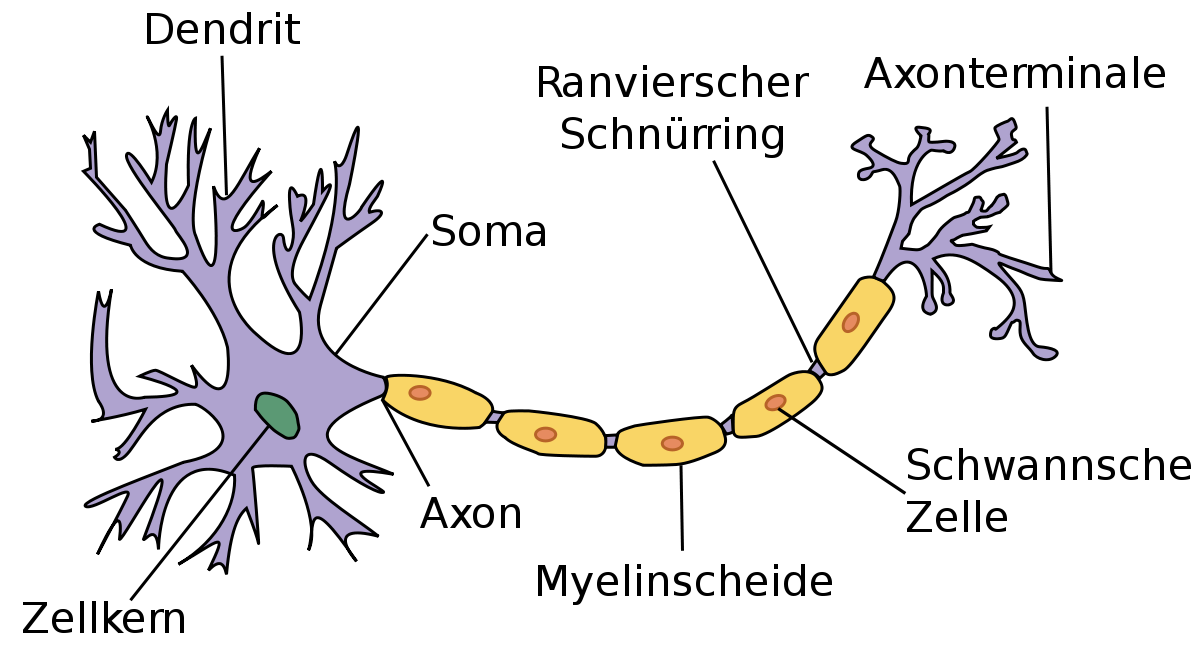
\includegraphics[scale=0.3]{Studienarbeit_F1/images/neuron.png}
    \caption[Vereinfachte Darstellung eines Neurons]{Vereinfachte Darstellung eines Neurons\footnotemark}
    \label{fig:neuron}
\end{figure}
\footnotetext{\citet{neuronimage}}
Mit Blick auf die Funktionsweise empfängt das Neuron die Erregung über ein weitverzweigtes System von Dendriten. Die Dendriten sind dabei Verbindungsschnittstelle zu den Synapsen beziehungsweise Axonterminalen vorgelagerter Neuronen. Die empfangenen Reize werden in Form von elektrischen Signalen über den Zellkörper (Soma) zum sogenannten Axonhügel weitergeleitet, der Verbindungsstelle des Axons mit dem Zellkörper. Sie gliedern sich dabei in Abhängigkeit von den auslösenden Synapsen in exzitatorische postsynaptische Potenziale (EPSP) mit einer erregenden Wirkung und inhibitorische postsynaptische Potenziale (IPSP) mit einer hemmenden Wirkung.\zitat{4f}{neuronbasics}\newline
Der Axonhügel bildet den zentralen Punkt der Summation der verschiedenen Signale. Hier werden die verschiedenen vielen ankommenden postsynaptischen Potenziale entsprechend ihrer erregenden oder hemmenden Wirkung aufsummiert und lösen gegebenenfalls ein Aktionspotenzial aus. Die Auslösung des Aktionspotenzials erfolgt nach dem sogenannten \glqq Alles-oder-nichts\grqq-Prinzip. Hierzu muss von der Überlagerung beziehungsweise Summation der ankommenden Signale ein gewisser Schwellenwert erreicht werden, welcher bei Überschreitung ein elektrisches Aktionspotenzial am Axonhügel auslöst. Die Form und der Verlauf des Aktionspotenzials sind dabei bei jeder Auslösung identisch und somit unabhängig vom Grad der Überschreitung des Schwellenwertes.\newline
Dieses Aktionspotenzial wird über eine Nervenfaser, das sogenannte Axon zu weiteren nachfolgenden Nervenzellen weitergeleitet.\zitat{22ff}{introductiontoneuralnetworks}\newline
Das Axon ist dabei von sogenannten Myelinscheiden umgeben, die in regelmäßigen Abständen von den ranvierschen Schnürringen unterbrochen sind. Diese nur bei Wirbeltieren vorkommenden Neuronenbestandteile ermöglichen durch die isolierende Wirkung der Myelinscheiden eine sogenannte saltatorische Erregungsleitung, welche sich durch eine besonders schnelle Übertragungsgeschwindigkeit des Aktionspotenzials gegenüber der kontinuierlichen Erregungsleitung auszeichnet.\zitat{1}{signalconduction}\newline
Die schlussendliche Übertragung der Erregung zwischen den Nervenzellen erfolgt in den meisten Fällen durch die Ausschüttung von chemischen Botenstoffen, den sogenannten Neurotransmittern an den Axonterminalen. Diese Ausschüttung wird durch die Ankunft des das Axon entlang gewanderten Aktionspotenzials ausgelöst. Diese Neurotransmitter erzeugen an den Dendriten der nachfolgend angeordneten Nervenzellen wieder eine erregende oder hemmende Wirkung.\zitat{22ff}{introductiontoneuralnetworks}\newline
Auf eine tiefer gehende Erläuterung biologischer Neuronen, insbesondere hinsichtlich ihrer biochemischen Funktionsweise, wird an dieser Stelle verzichtet, da dies für den Rahmen dieser Arbeit nicht zielführend wäre. %%Hier kann evtl. auch noch ein Buchverweis eingefügt werden, wenn man es für notwendig hält. So nachdem Schema: Auf eine genauere Erläuterung der Funktionsweise biologischer Neuronen wird, mit Verweis auf weiterführende Literatur [Verweise], verzichtet, da dies für den Rahmen dieser Arbeit nicht zielführend wäre.
\subsection{Künstliches Neuron}
\label{künstliches_neuron}
%Fully Corrected
Die Grundstruktur und theoretische Funktionsweise eines künstlichen Neurons, welches die Grundlage künstlicher neuronaler Netze bildet, orientiert sich in großem Maße an seinem biologischen Äquivalent. Seine Funktions- beziehungsweise Arbeitsweise kann anhand dem in \ref{fig:technicalneuron} abgebildeten Modell des Selbigen nachvollzogen und veranschaulicht werden.
%aineuron
\begin{figure}[H]
    \centering
    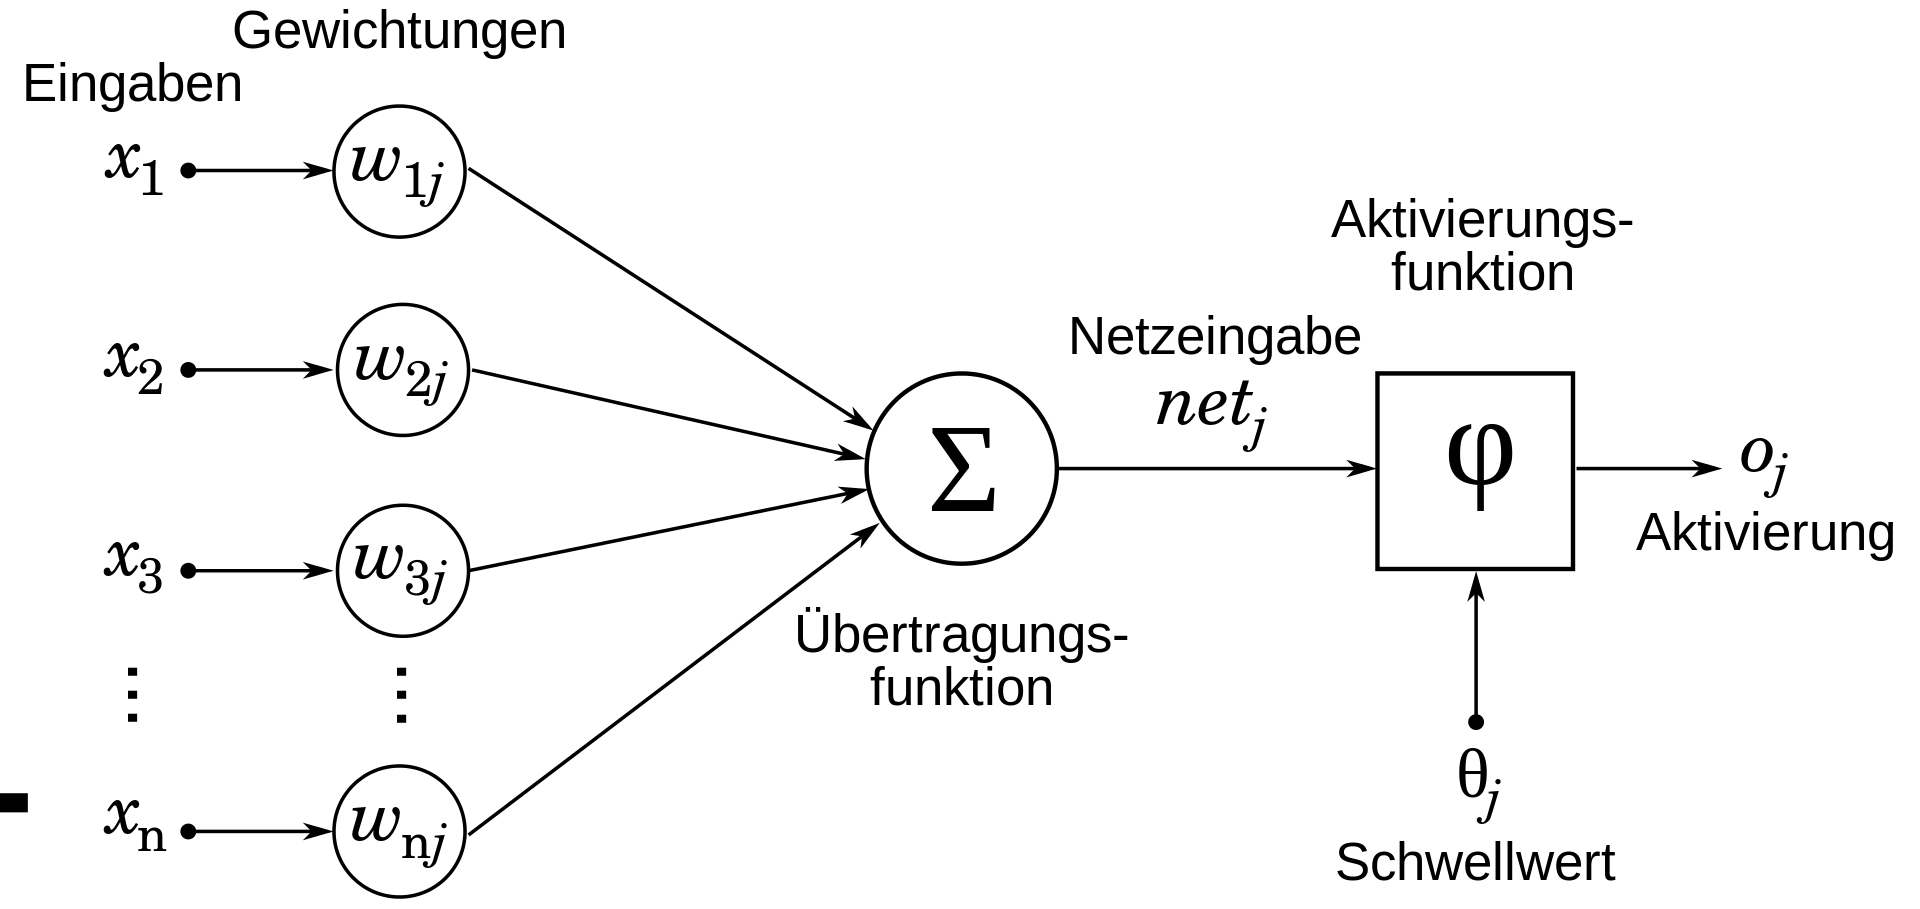
\includegraphics[scale=0.2]{Studienarbeit_F1/images/NeuronModel.png}
    \caption[Schaubild eines künstlichen Neurons]{Schaubild eines künstlichen Neurons\footnotemark}
    \label{fig:technicalneuron}
\end{figure}
\footnotetext{\citet{aineuron}}
Ein solches künstliches Neuron kann eine Vielzahl von Eingabewerten besitzen, welche entsprechend \ref{fig:technicalneuron} mit $x_1$ bis $x_n$ bezeichnet werden. Diese Eingabewerte werden mit zugehörigen Kantengewichten verrechnet, die das Maß des Einflusses der jeweiligen Eingabe auf das Neuron festlegen. Diese Gewichte werden mit $w_{1j}$ bis $w_{nj}$ bezeichnet.\\
Mit Blick auf das biologische Neuron lässt sich dieser Aspekt grundlegend mit den verschiedenen Arten der postsynaptischen Potenziale vergleichen.\zitat{5f}{neuronbasics}\\
Die Übertragungsfunktion erfüllt die Anforderung der Berechnung der Netzeingabe $net_j$. Dieser Wert repräsentiert dabei die Kumulierung aller Eingaben in Kombination mit den entsprechenden Gewichten. Mathematisch lässt sich dieser Sachverhalt beschreiben mit folgender Formel:\\
\begin{subequations}
    \begin{align}
    net_j = \sum\limits_{i=1}^n x_i \cdot w_{ij}
    \end{align}
Mit Blick auf das biologische Äquivalent ist dies mit der zuvor erläuterten Funktion des Axonhügels zu vergleichen.\\
Die Aktivierungsfunktion $\varphi$ ermittelt auf Grundlage der Netzeingabe $net_j$ und eines Schwellenwertes $\theta_j$ eine resultierende Aktivierung $o_j$. Demnach ergibt sich die Aktivierung $o_j$ eines Neurons und damit der Wert, der an potenziell nachfolgende Neuronen weitergeleitet wird, entsprechend:\\
    \begin{align}
        o_j = \varphi(net_j + \theta_j)
    \end{align}
Für die Aktivierungsfunktion $\varphi$ können verschiedene grundlegende Funktionen verwendet werden.\zitat{29ff}{introductiontoneuralnetworks} Nachfolgend werden die grundlegenden Arten von Aktivierungsfunktionen dargestellt. %Fully Corrected
\begin{itemize}
    \item \textbf{Heaviside-Funktion}:\\
    Die nachdem britischen Mathematiker und Physiker \glqq Oliver Heaviside \grqq benannte Funktion ist die grundlegendste Aktivierungsfunktion eines künstlichen Neurons. Alternative Bezeichnungen sind Treppen-Funktion oder Step-Funktion.\\
    Sie nimmt für alle Werte $v$ für die gilt $v < 0$ den Wert $0$ an, während sie für alle $v \geq 0$, den Wert $1$ an nimmt.
    Sie ergibt sich somit entsprechend
    \begin{align}
    \varphi(v) = \begin{cases}
            0 : v < 0 \\
            1 : v \geq 0
            \end{cases}
    \end{align}
    \begin{figure}[h]
        \centering
    \begin{tikzpicture}
    \begin{axis}[
    xmin = -1, xmax=1,
    ymin = -0.1, ymax=1.1,
    xtick={-1,-0.5,0,0.5,1}]
    \addplot[color=red]
    coordinates {(-1,0)(-0.5,0)(-0.00000001,0)(0,1)(0.5,1)(1,1)};
    \addlegendentry{Heaviside}
    \end{axis}
    \end{tikzpicture}
    \caption{Schaubild der Heaviside-Funktion}
    \end{figure}\\
    %ToDo, den Plot noch ein bisschen hübscher machen. ->"Bisschen mehr Luft um das Schaubild drum rum und die Linie des Graphen auch etwas dicker
    %ToDo Hier noch ein matplotlib Schaubild einfügen
    Die Verwendung dieser Aktivierungsfunktion erzeugt bei einem künstlichen Neuron ein Verhalten, welches dem \glqq Alles-oder-nichts\grqq-Verhalten seiner biologischen Vorbilder gleicht. Das künstliche Neuron erzeugt nur dann eine Aktivierung, wenn der Schwellenwert erreicht ist. Auch ist der Wert der Aktivierung nicht vom Grad der Überschreitung des Schwellwertes abhängig, was dem bei jeder Auslösung identischen Verlauf des Aktionspotenzials entspricht. Die Aktivierung bleibt entweder aus oder ist in vollem Umfang vorhanden, es existiert dabei keine Zwischenstufe.\\
    Der Gradient der Heaviside-Funktion ergibt sich über den gesamten Definitionsbereich zu null. Dadurch ist es nicht möglich, ein neuronales Netz nach dem Konzept der Fehler-Backpropagation zu trainieren. Diese Eigenschaft sorgt dafür, dass der Einsatz der Heaviside-Funktion in der Praxis meist vermieden wird.\zitat{2}{ImprovingNeuralNetworks} 
    Ein gängiger Anwendungsfall dieser Funktion findet sich Kontext der Single-Output-Networks im Zuge der binären Klassifikation.\zitat{3}{2021ReviewandComparison}%Keine Ahnung ob das richtig zitiert ist
    \item \textbf{Sigmoid-Funktion:}\\
    Eine weitverbreitete und in der Praxis häufig verwendete Aktivierungsfunktion stellt die sogenannte Sigmoid-Funktion dar. Weitere gängige Bezeichnungen sind logistische Funktion oder Quetschfunktion.\zitat{5f}{nwankpa2018activation}
    Sie stellt einen typischen Vertreter der \glqq S\grqq-förmigen Aktivierungsfunktionen dar. Diese zeichnen sich durch ihren nicht linearen Verlauf aus. Die typische Sigmoid-Funktion ist in Abhängigkeit der Eingabewerte $v$ definiert durch:
    \begin{align}
        \varphi(v) = \frac{1}{1+e^{-v}}
    \end{align}
    \begin{figure}[h]
        \centering
    \begin{tikzpicture}
        \begin{axis}[
        ]
            \addplot[color=red]{(1+exp(-x))^(-1)};
            \addlegendentry{Sigmoid}
        \end{axis}
    \end{tikzpicture}
    \caption{Schaubild der Sigmoid-Funktion}
    \end{figure}
    \\
    Bei der Sigmoid-Funktion handelt es sich um eine glatte Funktion, wodurch sie unendlich oft stetig differenzierbar ist.\\
    Sie kann grundsätzlich als Näherung der bei $0$ nicht differenzierbaren Heaviside-Funktion betrachtet werden, welche sich aufgrund ihrer einfachen Differenzierbarkeit innerhalb eines neuronalen Netzes gut verwenden lässt.\zitat{3f}{lederer2021activation} So ergibt sich die Ableitung der Sigmoid-Funktion zu:
    \begin{align}
        \frac{d}{dx}\varphi(v) = \varphi(v) \cdot (1-\varphi(v))
    \end{align}
    In der Praxis wird die Sigmoid-Funktion vor allem zur binären Klassifikation, aber auch zur Simulation von Funktionen eingesetzt. Im Allgemeinen eignet sie sich vor allem zur Anwendung in flachen neuronalen Netzen mit wenigen versteckten Schichten.\\
    Ein weiterer Vorteil der Sigmoid-Funktion neben der stetigen Differenzierbarkeit ist die Abbildung beliebiger Eingabewerte $v$ auf ein begrenztes Intervall von $(0,1)$, wodurch die Aktivierung des einzelnen Neurons innerhalb dieses Intervalls normiert ist.\\
    Dem entgegen steht der Nachteil, dass die Funktionswerte außerhalb des Intervalls [-2,2] kaum auf Änderungen der Eingabewerte reagiert. Somit ist der Gradient der Funktion außerhalb des angegebenen Intervalls sehr klein. Dadurch wird eine effektive Backpropagation erschwert, was dazu führen kann, dass das neuronale Netz sehr langsam oder sogar gar nicht lernt.\zitat{5f}{2021ReviewandComparison} Diese Auswirkung der kleinen Gradienten, welche eine nennenswerte Änderung der Gewichte im Zuge des Lernprozesses verhindert, werden durch eine höhere Anzahl von versteckten Ebenen verstärkt. Dadurch wird die Sigmoid-Funktion als Aktivierungsfunktion für derartige neuronale Netze beziehungsweise ihre versteckten Ebenen ungeeignet.\zitat{5}{nwankpa2018activation}\newpage
    \item \textbf{Rectified-Linear-Unit-Funktion:}\\
    Die Rectified-Linear-Unit-Funktion (ReLU) stellt die derzeit meist verwendete Aktivierungsfunktion innerhalb künstlicher neuronaler Netze dar.\zitat{8}{nwankpa2018activation} Sie wird teilweise als Rampen-Funktion bezeichnet. Sie nimmt für alle Eingabewerte $v$ für die gilt $v \leq 0$ den Funktionswert $0$ an und für alle $v > 0$ den Funktionswert $v$ an.\\
    Somit ist sie formal definiert durch:
    \begin{align}
        \varphi(v) = max(0,v) = \begin{cases}
                            0 \text{, wenn } v \leq 0\\
                            v \text{, wenn } v > 0
        \end{cases}
    \end{align}
    \begin{figure}[h]
    \centering
    \begin{tikzpicture}
    \begin{axis}[
        domain=-3:3,
        ]
        \addplot+[mark=none,red,domain=-3:0] {0};
        \addplot+[mark=none,red,domain=0:3] {x};
        \addlegendentry{ReLU}
    \end{axis}
\end{tikzpicture}
\caption{Schaubild der ReLU-Funktion}
\end{figure}
\\
    Ein wesentlicher Vorteil ist die einfache Implementierbarkeit der ReLU-Funktion und ihrer Ableitung, die sich zur Heaviside-Funktion ergibt. Sie erlauben dabei jeweils eine schnelle und kostengünstige Berechnung.\zitat{8}{lederer2021activation}
    Grund hierfür ist die simple Definition der Funktion, welche im Vergleich zur Sigmoid-Funktion keine Berechnung aufwendiger Divisionen oder Exponenten erfordert, was eine höhere Berechnungsgeschwindigkeit zur Folge hat. Weiterhin erlauben die linearen Eigenschaften der ReLU-Funktion eine effiziente Optimierung mittels Gradientenabstieg.\zitat{8f}{nwankpa2018activation}\\
    %Nachteile Leichtes Overfitting und DyingRelu-Problem, darauf eventuell auch noch eingehen und das erklären
    \item \textbf{Softmax-Funktion:}\\
    Eine weitverbreitete Aktivierungsfunktion aus dem Technologiefeld der neuronalen Netze stellt die Softmax-Funktion dar. Sie dient im Allgemeinen zur Berechnung einer Wahrscheinlichkeitsverteilung über einen Vektor reeler Zahlen. Hierbei erzeugt sie auf Basis des Eingabevektors $v$ der Länge $N$, eine Verteilung deren Einzelbestandteile zwischen $0$ und $1$ liegen und deren Summe sich zu $1$ ergibt.\\
    Sie ist formal definiert durch
    \begin{align}
        \varphi(v_i) = \frac{e^{v_i}}{\sum_{j=1}^{N} e^{v_j}}
    \end{align}
    Die Softmax-Funktion wird im Vergleich zur Sigmoid-Funktion zur multivariaten Klassifikation verwendet, während diese im Bereich der binären Klassifikation angewandt werden kann. Weiterhin wird sie in beinahe in sämtlichen Architekturen neuronaler Netze als Aktivierungsfunktion der Ausgabeschicht verwendet.\zitat{8}{nwankpa2018activation}
    
\end{itemize}
\end{subequations}

\subsection{Lernprozess künstlicher neuronaler Netze}\label{lernprozess}
Wie in Kapitel \ref{künstliches_neuron} erläutert, wird die Verarbeitung der Daten aus der vorherigen Schicht eines neuronalen Netzes im Wesentlichen über die Gewichte gesteuert. Um die Verhaltensweise der Ausgabe in einem Lernprozess zu adaptieren, muss demnach eine Methode zur Anpassung dieser gefunden werden. Für die Erläuterung eines Verfahrens zur Bewerkstelligung dessen wird zunächst die Struktur eines einfachen neuronalen Netzes, des sogenannten \gqq{multilayer perceptron} (MLP) eingeführt. Diese in Abbildung \ref{fig:MLP_structure} dargestellte Architektur umfasst Schichten von parallelen Neuronen, die jeweils vollständig mit ihrer vorherigen und nächsten Schicht verbunden sind. Die beliebig vielen Schichten zwischen der Eingabe- und Ausgabeschicht werden als versteckte Schicht zusammengefasst. Wird jede Kante des Graphen mit einer Gewichtung versehen, ergeben sich für die Aktivierungen eines jeden Neurons die bereits in Kapitel \ref{künstliches_neuron} erarbeiteten Zusammenhänge. Die Komposition mehrerer Schichten mit einer nicht linearen Aktivierungsfunktion für jedes Neuron der versteckten Schicht ermöglicht das Approximieren beliebiger Funktionen mit einer Genauigkeit, die von den genauen Parametern des Netzes abhängt.\footnote{Vgl. \cite{goodfellow_deep_learning} S.164-166} Diese Eigenschaft liefert die Begründung für die Nützlichkeit derartiger neuronaler Netze, da sich eine Vielzahl von Problemen als komplexe Funktionen modellieren lassen. Weiterer Vorteil dieser Architektur ist die Möglichkeit der eleganten mathematischen Beschreibung des Systems. Da sich die Aktivierung eines jeden Neurons aus der Linearkombination der Neuronen-Ausgaben der vorherigen Schicht mit ihren korrespondierenden Kantengewichten zum betrachteten Neuron ergibt, kann die Aktivierung eines einzelnen Neurons als Skalarprodukt implementiert werden. Die Aktivierungen einer gesamten Schicht lassen sich demnach durch mehrere Skalarprodukte der Ausgaben der vorherigen Schicht mit den Gewichten für alle gesuchten Neuronen berechnen. 
\begin{figure}[h]
    \centering
    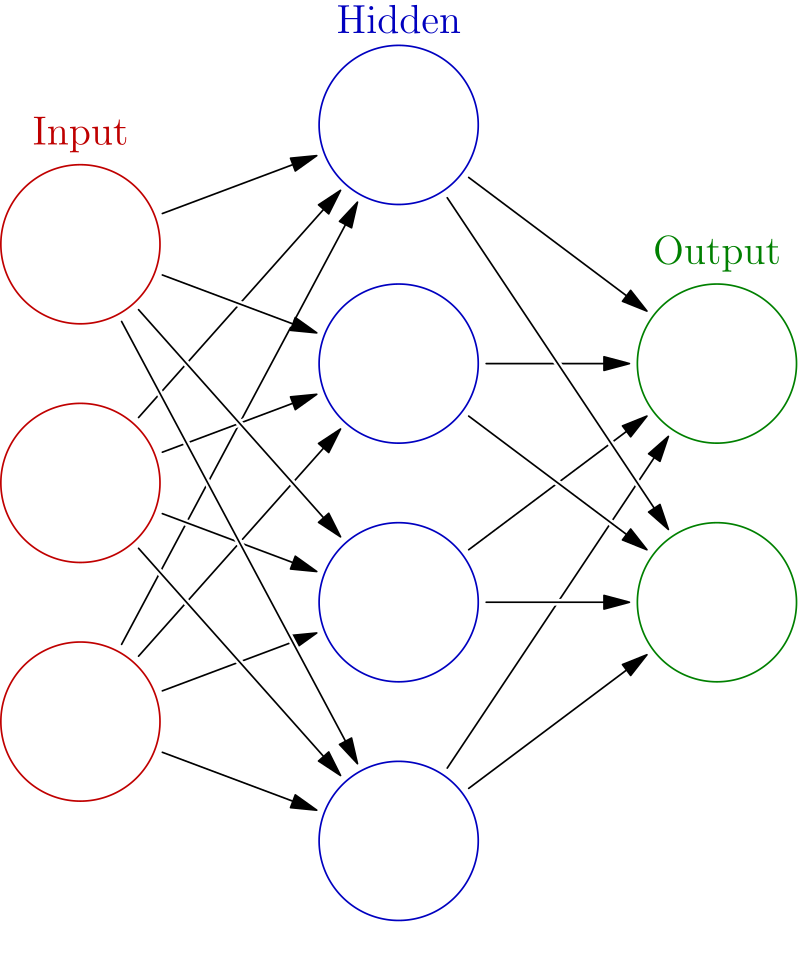
\includegraphics[scale=0.2]{Studienarbeit_F1/images/Neural_Network_Structure.png}
    \caption{Neuronenstruktur eines MLP}
    \label{fig:MLP_structure}
\end{figure}
Das Bilden von Skalarprodukten eines Vektors mit mehreren anderen Vektoren und das Sammeln der Ergebnisse in einem neuen Vektor ist mathematisch nichts anderes als eine Matrizenmultiplikation. Die Vorwärtspropagierung einer Eingabe in das Netz um eine Schicht lässt sich damit effizient als Matrizenmultiplikation mit anschließender, komponentenweiser Anwendung der Aktivierungsfunktion im Ergebnisvektor implementieren. In Matrixschreibweise ergibt sich die folgende Darstellung:
\begin{subequations}
    \begin{align}
        \label{eq:feedforward_matmul}
        \begin{bmatrix}
            w_{1,1} & w_{2,1} & \cdots & w_{n, 1}\\
            w_{1,2} & w_{2,2} & \cdots & \vdots\\
            \vdots & \vdots & \ddots & \vdots\\
            w_{1, m} & \cdots & \cdots & w_{n, m}
        \end{bmatrix}
        \cdot
        \begin{bmatrix}
            o_{i,1}\\
            \vdots\\
            o_{i,n}
        \end{bmatrix}
        =  
        \begin{bmatrix}
            a_{j, 1}\\
            \vdots\\
            a_{j, m}
        \end{bmatrix}
    \end{align}
    \begin{align}
        \label{eq:feedforward_activation}
        \begin{bmatrix}
            \varphi(a_{j, 1})\\
            \vdots\\
            \varphi(a_{j, m})
        \end{bmatrix} 
        =
        \begin{bmatrix}
            o_{j, 1}\\
            \vdots\\
            o_{j, m}
        \end{bmatrix}
    \end{align}
\end{subequations}
Eine Zeile in der Gewichtsmatrix repräsentiert die Gewichte aller Kanten, die zu einem Neuron der nächsten Schicht hinführen, während alle Spalten die Kantengewichte von einem Neuron der vorherigen Schicht hinweg darstellen. Durch die Multiplikation der Outputs der vorherigen Schicht \(i\) ergeben sich die Aktivierungen der nächsten Schicht \(j\), welche durch die komponentenweise Anwendung der nicht linearen Aktivierungsfunktion \(\varphi\) zu den Outputs der Schicht \(j\) werden.\\
Aus diesem Schema der Vorwärtsverarbeitung muss nun eine Methode zur Anpassung der Gewichte infolge eines Lernbeispiels abgeleitet werden, da nur so eine für das daliegende Problem passende Funktionsapproximation erreicht werden kann.
Für diesen Ansatz wird zunächst ein Sollwert bei der Ausgabe des Netzes benötigt. Dieser repräsentiert bei gegebener Eingabe in das Netz das final gewünschte, also korrekte Ergebnis. Die Abweichung vom Sollwert zum Istwert liefert eine Metrik zur Beurteilung der Performance des Netzes und kann verwendet werden, um die Gewichte in solch einer Weise anzupassen, dass der Wert der Fehlerfunktion minimiert wird. Der hierfür verwendete Algorithmus ist als \gqq{stochastic gradient descent} bekannt. Kern der Überlegung ist es, dass das Finden eines Tiefpunktes der Fehlerfunktion darüber implementiert werden kann, dass die Änderungsrate des Fehlers in Abhängigkeit der einzelnen Gewichte über die Anwendung der Kettenregel berechnet wird. Die Ableitungen werden in einem Vektor zusammengetragen und repräsentieren den Gradienten der Fehlerfunktion in Abhängigkeit der Gewichte. Der Gradient zeigt stets in die Richtung des stärksten Anstiegs eines Skalarfelds, somit resultiert aus der Änderung der Gewichte in Richtung des negativen Gradienten eine Annäherung an einen Tiefpunkt, der Fehler wird also minimiert. Das analytische Ermitteln der Ableitungen nach den Gewichten wird im Folgenden am Beispiel eines Ausgabewertes des Netzes illustriert. Die Ausgabe eines Neurons berechnet sich im allgemeinen Fall nach \ref{eq:feedforward_matmul} und \ref{eq:feedforward_activation} aus der Verkettung von zwei Funktionen, nämlich aus der gewichteten Summe aus den vorherigen Aktivierungen und der Anwendung der Aktivierungsfunktion. Zusätzlich muss die Anwendung der Fehlerfunktion nach der Ausgabeschicht bedacht werden. Ist also die nötige Anpassung des Gewichtes zwischen dem ersten Neuron der vorletzen und dem ersten Neuron der letzten Schicht gesucht, muss der folgende Ausdruck berechnet werden:
\[\frac{\partial E}{\partial w_{ij}} = \frac{\partial E}{\partial o_j} \cdot \frac{\partial o_j}{\partial a_j}\cdot \frac{\partial a_j}{\partial w_{ij}}\]
In Prosa lässt sich der Term insofern erklären, dass zunächst die Fehlerfunktion nach der Neuronenausgabe, dann die Neuronenausgabe nach der Aktivierungsfunktion und zuletzt die Aktivierung des Neurons nach dem gewünschten Gewicht abgeleitet wird. Es resultiert das Verhältnis der Änderung in der Fehlerfunktion zu einer Änderung des relevanten Gewichtes. Theoretisch kann diese Kette an Kompositionen bis zur Eingabeschicht des Netzes zurückverfolgt werden, was für die Ableitung nach den sich dort befindenden Gewichten auch praktiziert wird. Für Gewichte, welche sich in einer früheren Schicht befinden, müssen verschiedene \gqq{Wege} durch das Netz addiert werden, da so ein Gewicht die Fehlerfunktion über mehrere Neuronen beeinflusst.\footnote{Vgl. \cite{goodfellow_deep_learning} S.200 - 213}
Die Details dieser Berechnungen lassen sich beispielsweise in \cite{goodfellow_deep_learning} nachlesen und sind im Wesentlichen triviale weitere Betrachtungen, die auf denselben Ansatz der Anwendung der Kettenregel zur Rückverfolgung der Verbindungen des Netzwerkes zurückgehen.
Moderne Bibliotheken\footnote{Bekannte Beispiele sind PyTorch oder Tensorflow} für die Entwicklung neuronaler Netze sind im Kern Programmierhilfen, die das Definieren von Schichten vereinfachen und die relevanten Ableitungen automatisch berechnen.

\subsection{Diskrete Eventsimulation}
% Fully corrected
Die Möglichkeit einer Simulation durch das Erstellen eines geeigneten Modells zur Analyse birgt umfassende Vorteile gegenüber der reinen Observierung des realen Systems. Beispielsweise enthält der Prozess des Aufbauens des Modells bereits das Potential, die Zusammenhänge im System genauer zu verstehen, aber auch die Notwendigkeit für Details zu erkennen. Weiter erlaubt das Verwenden eines Modells die kontinuierliche Wiederholung der Vorgänge im System bei exakt gleichen Verhältnissen sowie das minimale Anpassen von Parametern, um deren Auswirkungen im untersuchten System umfassender zu verstehen. In diesem Fakt zeichnet sich auch ab, dass das Beeinflussen des Systems in einem Modell leichter fällt als in einer realen Umgebung. Ein weiterer Vorteil der Simulation liegt im Umstand der Schnelligkeit, denn die Simulation kann bei Bedarf ohne Verlust von Information schneller abgespielt werden als das reale Vorbild. Optional kann der Ablauf aber auch verlangsamt werden, um somit wiederum Einblicke zu gewinnen, welche im echten Umfeld nicht möglich sind.\zitat{}{discrete_event_sim_fishman}
\\\\
Ein methodischer Ansatz, eine Simulation zu erstellen, ist durch die diskrete Eventsimulation beschrieben. Hierbei wird versucht, das reale Modell, welches meist von chronologischer Kontinuität geprägt ist, in zeitlich unabhängige feste Ereignisse zu unterteilen, welche aber trotzdem die originale Reihenfolge beibehalten. Wie bei jeder Simulation bleibt dieser Ansatz aber immer eine Annäherung der Wirklichkeit und es ist bei der Implementation auf den gewählten Detailgrad zu achten. Sollte zu stark auf Details im Modell verzichtet werden, verbessert dies zwar die Laufzeit und die Flexibilität des Modells, dennoch leidet aber die Aussagekraft der Ergebnisse darunter. Um in diesem Fall den korrekten Pfad zu wählen, muss zunächst die Zielsetzung des Modells definiert werden, um darauf abzuleiten, ob das Modell sich entsprechend verhält oder der Abstraktionsgrad zu hoch gewählt worden ist.

\subsection{Formel 1} %Alex
% Fully corrected
Die Formel 1 ist eine seit 1950 existierende Rennserie, welche jährlich stattfindet und Rennen global abhält. Dabei besteht ein Rennwochenende aus verschiedenen Trainings sowie einem Qualifying, um die Startreihenfolge für das darauf folgende Rennen festzulegen. Antreten tun dabei verschiedene Teams, welche entweder direkt von Automobilherstellern betrieben werden oder von Externen mit jeweils zwei Autos mit zugehörigen Fahrern / Fahrerinnen pro Team. Die Entwicklung der Autos erfolgt durch jedes Team selbst in einem vorgegebenen Rahmen von Regularien, welche durch die FIA (Federation Internationale de l’Automobile) dem Veranstalter der Formel 1 bestimmt werden. 
\\\\
Nachfolgend werden einzelne Aspekte der Formel 1 aus der technischen Sicht sowie einige Regularien vorgestellt, welche diese Arbeit maßgeblich beeinflussen und besonders bei der Entwicklung des simulierten Trainingsumfeldes relevant sind überhaupt mit der Realität vergleichbare Ergebnisse zu erhalten. Dabei werden dennoch Vereinfachungen getroffen, deren Behandlung und Implementation nicht im zeitlichen Umfang dieser Arbeit realisierbar sind. Beispielsweise werden Wettereinflüsse vernachlässigt, weshalb diese nicht im Rahmen der Formel 1 weiter beschrieben werden.

\subsubsection{Reifen} %Alex

Seit 2019 stehen den verschiedenen Formel 1 Teams pro Rennwochenende nur drei verschiedene Reifenmischungen zur Verfügung, welche vom italienischen Reifenhersteller Pirelli entwickelt und bereitgestellt werden. Diese unterliegen den Bezeichnungen \glqq Soft\grqq{}, \glqq Medium\grqq{} und \glqq Hard\grqq{} in Relation zur Zusammenstellung der Gummimischung des jeweiligen Reifentyps. Entsprechend der Bezeichnung verhalten sich die Reifen auch im Rennbetrieb, so entspricht der \glqq Soft\grqq{} dem weichsten Reifen der drei Kategorien und erlaubt somit den größten Haftungskoeffizient und damit die beste Traktion. Durch die Weichheit verschleißt dieser Reifen aber wesentlich schneller und muss somit früher wieder gewechselt werden. Diesbezüglich verhalten sich die weiteren Mischungen bis zum \glqq Hard\grqq, welcher besonders langlebig ist aber nur eine begrenzte Rundenzeit erlaubt. Die Reifen entsprechen dabei jedem Rennwochenende einer anderen Mischung, um an die Charakteristiken der jeweiligen Rennstrecke angepasst zu sein. Der Grundgedanke von weich zu harter Mischung bleibt dabei aber erhalten und wird entsprechend nur als solcher kommuniziert.\\
Dabei ist die Gesamt-Anzahl der Reifen pro Auto limitiert, worauf aber weiterführend in dieser Arbeit keine weitere Rücksicht genommen wird.

\subsubsection{Regeln} %Alex
% Fully corrected
Das für diese Arbeit relevante Reglement ist rein durch die Notwendigkeit beschrieben, dass jedes Auto pro Rennen mindestens zwei verschiedene Reifenmischungen fahren muss. Heißt ein Auto, welches auf harten Reifen startet wird disqualifiziert, sollte es auf diesen Reifen das Rennen beenden. Es müssen also mindestens einmal pro Rennen die Reifen gewechselt werden und dabei auch verschiedene Mischungen gefahren werden. Das bedeutet, es darf auch nicht ein ganzes Rennen auf drei Reifensätzen der Mischung "weich" gefahren werden.
Weitere Regeln stehen in keinem direkten Zusammenhang zu dieser Arbeit und können entsprechend vernachlässigt werden.

\subsubsection{Renngeschehen}\label{sec:race_behaviour} %Alex
% Fully corrected
Ein Rennen in der Formel 1 besteht aus einer festen Anzahl an Runden, welche absolviert werden müssen. Wer zuerst die geforderte Rundenzahl erfüllt, gewinnt das Rennen. Die restlichen Plätze werden abhängig von der weiteren Zieldurchfahrt bestimmt. Es gibt zwar zeitliche Limitationen, nach welchen die Rennen unabhängig vom Rundenzähler beendet werden, diese sind aber in dieser Arbeit nicht zu berücksichtigen sowie die Sonderregelung für überrundete Autos.\\\\
Ein Auto braucht für eine Runde eine gewisse Zeit in welcher die Reifen entsprechend durch die Belastung abnutzen. Mit zunehmender Abnutzung der Reifen verlieren diese an Haftungseigenschaften und die Traktion für das Fahrzeug wird schlechter, was zwangsweise zu einer langsameren Rundenzeit führt. Darauf basierend muss ein Auto nach einem Rahmen an Runden wieder an die Box, um den Reifen zu wechseln und somit einen Reifenplatzer zu vermeiden, welcher das Rennen für das jeweilige Fahrzeug beenden könnte. In diesem Umstand liegt der Existenzgrund der Rennstrategie, welche das Ziel besitzt, möglichst vorteilhaft den Boxenstopp einzuplanen, um möglichst wenig Zeit in Bezug zur gesamten Rennzeit zu verlieren.\\\\
Ein besonderer Aspekt, welcher hierbei mit berücksichtigt werden muss, ist der Umstand, dass moderne Formel 1 Autos große Schwierigkeiten beim Verfolgen eines vorausfahrenden Autos haben. Die durch das vorausfahrende Auto verwirbelte Luft reduziert die aerodynamische Effizienz des eigenen Fahrzeugs und reduziert somit die Haftung auf dem Boden. Dies bedeutet eine geringere Kurvengeschwindigkeit und somit eine langsamere Rundenzeit. Sollte dennoch versucht werden, die Geschwindigkeit des vorausfahrenden Fahrzeugs mithalten zu wollen, so muss der eigene Reifen stärker strapaziert werden, was wiederum zu einem schnelleren Verschleiß des Reifens führt. Zudem kann ein Reifen in dieser Situation schneller überhitzen, was wiederum weniger Traktion und schnelleren Verschleiß bedeutet. Das vorausfahrende Fahrzeug sollte also möglichst schnell überholt werden, um das eigene Rennen nicht weiter zu kompromittieren.\\\\
Beim Überholen ist zusätzlich zu beachten, dass das vorausfahrende Auto meist nicht freiwillig die Position abgibt. Dies bedeutet, dass zwischen den Autos ein Kampf um die Position stattfindet, welcher besonders durch die zur Verfügung stehende Traktion eines Autos bestimmt wird. So fällt es einem Auto auf frischen weichen Reifen verhältnismäßig leichter an einem Fahrzeug auf alten harten Reifen vorbeizukommen, als im Falle von gleicher Bereifung für beide Fahrzeuge. In diesem Fall kann es auch dazu führen, dass der Überholvorgang nicht erfolgreich bleibt und das hintere Auto nicht schneller die Runde vollenden kann als das Auto davor.

\subsection{Polynominale Regression}\label{sub: polynominal_regression}
% Fully corrected
Die polynominale Regression oder auch \gqq{Polynominal Least Square Fit} beschreibt ein Verfahren, um näherungsweise eine Funktion zu generieren, welche bestmöglich zu einem gegebenen Datensatz passt. Dabei versucht das Verfahren die Varianz zwischen den späteren angenäherten Werten pro Datensatz und den tatsächlichen Werten der Eingangsdaten zu minimieren.\\
Der grundlegende Ansatz einer Regression basiert auf der allgemeinen Gleichung einer Funktion, welche in Gleichung \ref{default_func_term} dargestellt ist. Hierbei sind alle Parameter $a$ unbekannt und müssen entsprechend dem gewünschten Grad der Funktion auf Basis der gegebenen Datenpunkte bestimmt werden.
\begin{equation}\label{default_func_term}
    y = a_k*x^k + a_{k-1} * x^{k-1} + ... + a_1*x + a_0
\end{equation}
Ein Ansatz, dieses Problem zu lösen ist, jede Gleichung aufzustellen, welche das System erfüllen muss und anschließend nach den gesuchten Parametern aufzulösen. Dies bedeutet, jeden einzelnen gegebenen Punkt in die allgemeine Funktionsgleichung einzusetzen und das resultierende Gleichungssystem zu lösen. Hierbei kann auf die Matrix-Schreibweise eines Gleichungssystems zurückgegriffen werden. Dies dient der Übersichtlichkeit und erleichtert die methodische Lösung des Systems bei großen Datenmengen.

\begin{subequations}
    \begin{align}\label{eq: approch_poly_reg}
    \begin{bmatrix}
    1 & x_1 & \cdots   & x_1^k \\ 
    1 & x_2  & \cdots  & x_2^k \\ 
    \vdots  & \vdots  & \ddots  & \vdots \\ 
    1 & x_n & \cdots  & x_n^k
    \end{bmatrix}
    \begin{bmatrix}
    a_0 \\
    a_1 \\
    \vdots \\
    a_k
    \end{bmatrix}
    =
    \begin{bmatrix}
    y_0 \\
    y_1 \\
    \vdots \\
    y_k
    \end{bmatrix}
    \end{align}
\\
Zur allgemeinen Lösung der Gleichung \ref{eq: approch_poly_reg} muss auf die von Roger-Moore beschriebene Pseudo-Inverse zurückgegriffen werden, welche es erlaubt, eine Division durch eine nicht quadratische Matrix durchzuführen. Hierzu wird die transponierte Matrix von links auf beide Seiten der Gleichung multipliziert, um somit die Gleichung weiterhin zu erfüllen, dabei aber eine quadratische Matrix als Produkt der zu invertierenden Matrix und ihrer Transponierten zu erzeugen. Diese Matrix kann dann durch ihre quadratischen und symmetrischen Eigenschaften invertiert werden und somit zur Lösung der Gleichung genutzt werden.\zitat{}{polynomial_regression}
%\cite{polynomial_regression}

    \begin{align}\label{eq: pseudo_inverse_poly_reg}
    \begin{bmatrix}
    1 & 1 & \cdots & 1 \\ 
    x_1 & x_2  & \cdots  & x_n \\ 
    \vdots  & \vdots  & \ddots  & \vdots \\ 
    x_1^k & x_2^k & \cdots  & x_n^k
    \end{bmatrix}
    \begin{bmatrix}
    1 & x_1 & \cdots   & x_1^k \\ 
    1 & x_2  & \cdots  & x_2^k \\ 
    \vdots  & \vdots  & \ddots  & \vdots \\ 
    1 & x_n & \cdots  & x_n^k
    \end{bmatrix}
    \begin{bmatrix}
    a_0 \\
    a_1 \\
    \vdots \\
    a_k
    \end{bmatrix}
    =
    \begin{bmatrix}
    1 & 1 & \cdots & 1 \\ 
    x_1 & x_2  & \cdots  & x_n \\ 
    \vdots  & \vdots  & \ddots  & \vdots \\ 
    x_1^k & x_2^k & \cdots  & x_n^k
    \end{bmatrix}
    \begin{bmatrix}
    y_0 \\
    y_1 \\
    \vdots \\
    y_k
    \end{bmatrix}
    \end{align}
    
    \begin{align}\label{eq: solution_poly_reg}
    \begin{bmatrix}
    n & \sum_{i=1}^{n} x_i & \cdots & \sum_{i=1}^{n} x_i^k \\ 
    \sum_{i=1}^{n} x_i & \sum_{i=1}^{n} x_i^2  & \cdots  & \sum_{i=1}^{n} x_i^{k+1} \\ 
    \vdots  & \vdots  & \ddots  & \vdots \\ 
    \sum_{i=1}^{n} x_i^{k} & \sum_{i=1}^{n} x_i^{k+1} & \cdots  & \sum_{i=1}^{n} x_i^{2k}
    \end{bmatrix}
    \begin{bmatrix}
    a_0 \\
    a_1 \\
    \vdots \\
    a_k
    \end{bmatrix}
    =
    \begin{bmatrix}
    \sum_{i=1}^n y_i \\
    \sum_{i=1}^n x_i y_i \\
    \vdots \\
    \sum_{i=1}^n x_i^k y_i
    \end{bmatrix}
    \end{align}
\end{subequations}
\\
In die resultierende Gleichung \ref{eq: solution_poly_reg} können jetzt die entsprechenden Summen der Datenpunkte eingesetzt und abschließend durch die Multiplikation mit der Inversen nach dem Vektor a aufgelöst werden. Die resultierenden Parameter in die allgemeine Funktionsgleichung \ref{default_func_term} eingesetzt ergeben dann die gewünschte Funktionsgleichung, welche nun die Datenmenge bestmöglich repräsentiert.\\
Das diese Lösung eine bestmögliche Näherung der Datenmenge darstellt, wird durch eine andere Herleitung der Gleichung \ref{eq: solution_poly_reg} offensichtlich. Hierbei werden Residuen genutzt. Ein Residuum beschreibt in der numerischen Mathematik den Abstand einer Funktion zu einem Punkt bei identischem Wert $x$.
\begin{subequations}
    \begin{align}\label{eq: def_residual}
        r = y_{dot} - y_{func}
    \end{align}
Dieser Ansatz basiert darauf, die allgemeine Funktionsgleichung \ref{default_func_term} in die allgemeine Form der Residuen einzusetzen und aufzusummieren, um damit die \gqq{Fitness} der gesamten Funktion auf die gesamte Menge der Datenpunkte untersuchen zu können. Aufgrund des Umstandes, dass die resultierenden Residuen positiv wie negativ sein können und somit sich in Summe wieder annullieren würden, werden die Ergebnisse quadriert, um dieses Problem zu umgehen, wie beispielsweise auch bei der Berechnung der Standardabweichung in der Statistik.
    \begin{align}\label{eq: complete_residuals_function}
        R^2 = \sum_{i=1}^n [y_i - (a_k*x_i^k + a_{k-1} * x_i^{k-1} + ... + a_1*x_i + a_0)]^2
    \end{align}
Um eine möglichst gut passende Funktion zur Datenmenge zu erhalten, muss der resultierende Wert $R^2$, welcher dann die gesamte \gqq{Fitness} der gewünschten Funktion repräsentiert, minimiert werden. Dies kann methodisch über die partielle Ableitung nach jedem einzelnen Parameter $a_k$ erreicht werden. 
    \begin{align}
        \frac{\partial(R^2)}{\partial(a_k)} = -2 \sum_{i=1}^n[y-(a_0+a_1x+...+a_k x^k)] = 0
    \end{align}
Entsprechend ergibt sich für jedes $a_k$ eine eigene Gleichung, welche zur Minimierung gleich null gesetzt werden muss. Eine anschließende Umformung und Darstellung des Gleichungssystems als Matrix ergibt dieselbe Gleichung \ref{eq: solution_poly_reg}.\zitat{}{math_poly_reg}
\end{subequations}
	\section{Umsetzung}
% Fully corrected!
Im Folgenden werden die verschiedenen Ansätze zur Lösung des Problems dieser Arbeit betrachtet und dargelegt. Dabei soll besonders die verschiedenen Möglichkeiten beleuchtet werden, um somit auch Vergleiche zwischen den Technologien anstellen zu können.\\\\
Als Vorbereitung zur Implementation und dem späteren Training gilt es zunächst eine Datengrundlage zu schaffen, auf welcher der Trainingsprozess stattfinden kann. Für diese Datengrundlage gilt der Anspruch, dass sie möglichst umfassend ist und somit im gesamtem Training der KI möglichst viele diverse Situationen abbildet, um somit den Trainingserfolg in der Theorie zu maximieren.\\
Damit dieser Anspruch erfüllt werden kann, aber gleichzeitig der benötigte Aufwand für das Sammeln der Daten sowie das Auswerten dieser minimal gehalten wird, bietet sich die Verwendung eines Simulators an. In diesem simulierten Umfeld kann die KI gegen sich selbst antreten und somit anhand dieser Erfahrungen lernen. Dies bedeutet, dass ein Modell geschaffen werden muss, welches der Realität möglichst gut entspricht, um somit die Lernergebnisse der KI überhaupt in der Realität nutzbar zu machen.\\\\
Mit dem funktionierenden Simulator kann dann die Entwicklung einer KI begonnen werden, welche mit dem simulierten Umfeld interagieren kann und dieses entsprechend die benötigten Informationen zur Entscheidungsfindung bereitstellt. Mit diesen Komponenten und einem Ansatz zur korrekten Bewertung der KI Entscheidungen im Lernprozess kann ein zielführendes Training der KI erfolgen.\\\\
Die KI-Entwicklung fußt zunächst auf einer Entscheidung der korrekten Technologien und Algorithmen für das vorliegende Problem. Im Weiteren können die einzelnen Parameter anhand von Daten des Lernprozesses eines Prototypen verfeinert werden, sodass schlussendlich für jeden verfolgten Ansatz eine belegbar optimale Performance erzielt wird.\\\\
Anschließend zur Entwicklung werden die verschiedenen Ansätze bewertet und gegenseitig in Kontext gesetzt, um somit abschließend einen möglichst geeigneten Prototypen vorstellen zu können.

\subsection{Technologie Entscheidung}
%Fully Corrected
Durch den Umstand, dass die bevorstehenden Aufgaben maßgeblich mit dem Umgang von Daten und der Implementation einer KI geprägt sind, wird zur Umsetzung im Folgenden hauptsächlich auf die Programmiersprache \gqq{Python} gesetzt. Diese zeichnet sich besonders bei der Implementation von künstlichen Intelligenzen durch bestehende und umfangreiche Bibliotheken aus. Zusätzlich ist die Kompetenz im Team der Autoren im Umgang mit Python sehr hoch und erleichtert somit den Einstieg in die künstliche Intelligenz.\\\\
%TODO umformulieren und ausbauen
Mit Blick auf die ausgewählte Programmiersprache stehen zur Umsetzung der KI verschiedene Bibliotheken zur Verfügung, die bereits Strukturen zur Implementierung neuronaler Netze bereitstellen.\\
Zweck eines solchen Frameworks ist es, die Entwicklung der Algorithmen des maschinellen Lernens zu Vereinfachen und dem Nutzer einen gewissen Grad an Abstraktion zu bieten, sodass er sich im Wesentlichen nicht um die zugrunde liegenden mathematischen Prinzipien entsprechend den Ausführungen in \ref{künstliches_neuron} und \ref{lernprozess} kümmern muss. Hierbei bieten im Allgemeinen verschiedene Bibliotheken einen unterschiedlichen Grad der Abstraktion.\\
Zur Entscheidung für ein geeignetes Frameworks werden nachfolgend die weitverbreiteten Bibliotheken Tensorflow und PyTorch betrachtet.
\begin{itemize}
    \item Tensorflow:\\\\
    Das ursprünglich als interne Lösung von Google entwickelte und seit 2015 veröffentlichte Machine-Learning-Framework Tensorflow gehört mit zu den verbreitetsten und bekannten Lösungen für die Implementierung neuronaler Netze. Als eine der wichtigsten Eigenschaften von Tensorflow gilt der Grad an Abstraktion, den der Entwickler %TODO nachdenken ob gendern
    durch die Verwendung dieser Bibliothek erreichen kann. So muss sich der Nutzende nicht mit den zugrunde liegenden Details neuronaler Netze auseinandersetzen, sondern kann sich auf die übergeordnete Logik des zu implementierenden Anwendungsfalls beziehungsweise des abzubildenden Modells konzentrieren. Weiterhin gilt Tensorflow als Framework, welches eine gute Erweiterbarkeit beziehungsweise Skalierbarkeit ermöglicht.
    Im Allgemeinen stehen Schnittstellen zur Verfügung, die die Verwendung verschiedenster Programmiersprachen im Zusammenspiel mit Tensorflow erlauben, darunter auch Python.\zitat{}{pytorchtensorflow}
    \\
    \item PyTorch:\\\\
    Die in erster Version 2018 veröffentliche Machine-Learning-Bibliothek PyTorch stellt eine Lösung mit wachsender Popularität und Verbreitung für die Realisierung neuronaler Netze dar. Sie basiert dabei zu wesentlichen Teilen auf dem mittlerweile veralteten LuaTorch, einer Bibliothek zur Durchführung wissenschaftlicher Berechnungen.\\
    PyTorch gilt als Bibliothek welche eine besonders python-typische Umsetzung neuronaler Netze ermöglicht und hierzu Interfaces bereitstellt, welche python-erfahrenen Entwicklern einen intuitiven Umgang mit dem Framework ermöglichen. Weiterhin gilt PyTorch als Framework welches sich durch seine Flexibilität auszeichnet, besonders hinsichtlich der Möglichkeiten des Debuggings und Testings.\zitat{}{pytorchtensorflow}
\end{itemize}
Mit Blick auf die vorgestellten Bibliotheken wurde sich für die Verwendung von PyTorch entschieden. Gründe hierfür sind zum einen die bereits erwähnte Kompetenz der Entwickler in der Programmiersprache Python, aus welcher sich durch die Verwendung von PyTorch eine schnelle Einarbeitung und intuitive Entwicklung ergibt. Ein weiterer positiver, wenngleich nicht entscheidungskritischer Aspekt ist die höhere Performance von PyTorch gegenüber dem Machine-Learning-Framework Tensorflow.\zitat{}{performancePytorchTensorflow}\\\\
Es ist anzumerken, dass trotz der Entscheidung für PyTorch die implementierten Algorithmen keine Funktionalitäten verwenden, die spezifisch für die gewählte Bibliothek sind. Somit lässt sich die nachfolgend dargestellte Umsetzung des neuronalen Netzes beziehungsweise der künstlichen Intelligenz grundsätzlich ohne Weiteres mithilfe von alternativen Bibliotheken und vergleichbaren Tools umsetzen.

\subsection{Rennsimulator}
% Fully Corrected
Um unsere KI trainieren zu können, bedarf es eine aussagekräftige Datengrundlage, welche umfassend diverse Situationen abbildet. Nur in diesem Fall kann die KI tatsächliche Strategien erlernen, welche als solche dann in den realen Anwendungsfall übertragen werden können. Da seit dem Jahr 2017 in der Formel 1 eine neue Art Reifen gefahren wird, welche an der Vorder- sowie Hinterachse am Fahrzeug breiter sind und zusätzlich aus moderneren Mischungen bestehen, können als reale Datengrundlage nur die Rennen von 2017 bis zum jetzigen Stand Ende 2021 benutzt werden. In diesem Zeitraum wurden die Mischungen vom Zulieferer der Reifen zwar leicht angepasst, dennoch wird hierbei aufgrund der identischen Abmessungen zu den Reifen bis Ende der Saison 2021 von einer gegebenen Vergleichbarkeit ausgegangen. Entsprechend stehen nur 100 Rennen als Datengrundlage zur Verfügung, was für das Training einer KI unzureichend ist und uns somit zwingt, eine andere Methode zu wählen, um eine aussagekräftige und möglichst diverse Umgebung zu schaffen, in welcher die KI die umfassenden Möglichkeiten eines Formel 1 Rennens kennen und verstehen lernen kann. Daher wurde im Team die Entscheidung getroffen, einen Simulator für ein Rennen zu schreiben, welcher auf Modellen und Abstraktionen beruht, die durch die Erhebung der Datenmenge über den Zeitraum von 2018 - 2021 erfolgen. Diese Modelle werden dann genutzt, um beispielsweise den Reifenverschleiß pro Runde simulieren zu können und sollen dabei das Verständnis des Zusammenhangs zwischen der Abnutzung des Reifens und der noch bestmöglichen Rundenzeit liefern. Gerade dieser Zusammenhang ist ein Kernpunkt in Bezug auf den Erfolg des Simulators, da der Traktionsverlust pro Runde durch den zunehmend verschlissenen Reifen maßgeblich die Rennstrategie und den optimalen Zeitpunkt des Boxenstopps bestimmt.

\subsubsection{Anforderungen}
% Fully corrected!!!
% Realitätsnah, Zeitlich weniger Aufwand -> Arbeit soll KI nicht Sim, Skalierbar -> weil ausgeklammert,  
Die Anforderungen gegenüber des Simulators beschränken sich im Kern auf eine möglichst genaue Abstraktion der Wirklichkeit, um somit die Relevanz und Nutzbarkeit der von uns entwickelten KI sicherzustellen und zu gewährleisten. Aufgrund des zeitlichen Rahmens dieser Arbeit wird hierbei aber die Notwendigkeit des Ausklammerns von möglichen Einflüssen genannt, um damit zu Beginn der Arbeit die Komplexität in der Entwicklung und später im Training der KI zu reduzieren und somit sich zunächst auf einen aussagekräftigen Prototypen zu beschränken. Beispielsweise könnte initial auf jegliche Abbildung von Wetter und Luft- wie Streckentemperatur verzichtetet werden und dennoch ein robuster Simulator für trockene Wetterverhältnisse geschaffen werden. Folgend dieser möglichen Notwendigkeit der Reduktion von berücksichtigen Faktoren soll bei der Entwicklung des Simulators besonders in der Architektur auf die Skalierbarkeit dieser geachtet werden, um somit die nachfolgende Erweiterung ohne umfassenden zeitlichen Aufwand zu ermöglichen.

Die in dieser Arbeit untersuchten Faktoren und somit Anforderungen an unseren Simulator sind umfassend durch den Reifenverschleiß, der individuellen Leistung eines einzelnen Fahrzeuges in Kombination mit dem Fahrer und den Wechselwirkungen der Fahrzeuge untereinander gegeben. Diese Einflüsse sollen durch das geeignete Modell im Simulator widergespiegelt und berücksichtigt werden.

\newpage %TODO may be not necessary; shall prevent fig:sim_architecture to behave random
\subsubsection{Architektur} \label{sim_architecture_header}
% Fully corrected
% Diskrete Eventsimulation, gewährleisten von Skalierbarkeit, OOP, Performance, Technologie Entscheidung Python weil Anbindung an KI Libs
\begin{figure}[H]
    \centering
    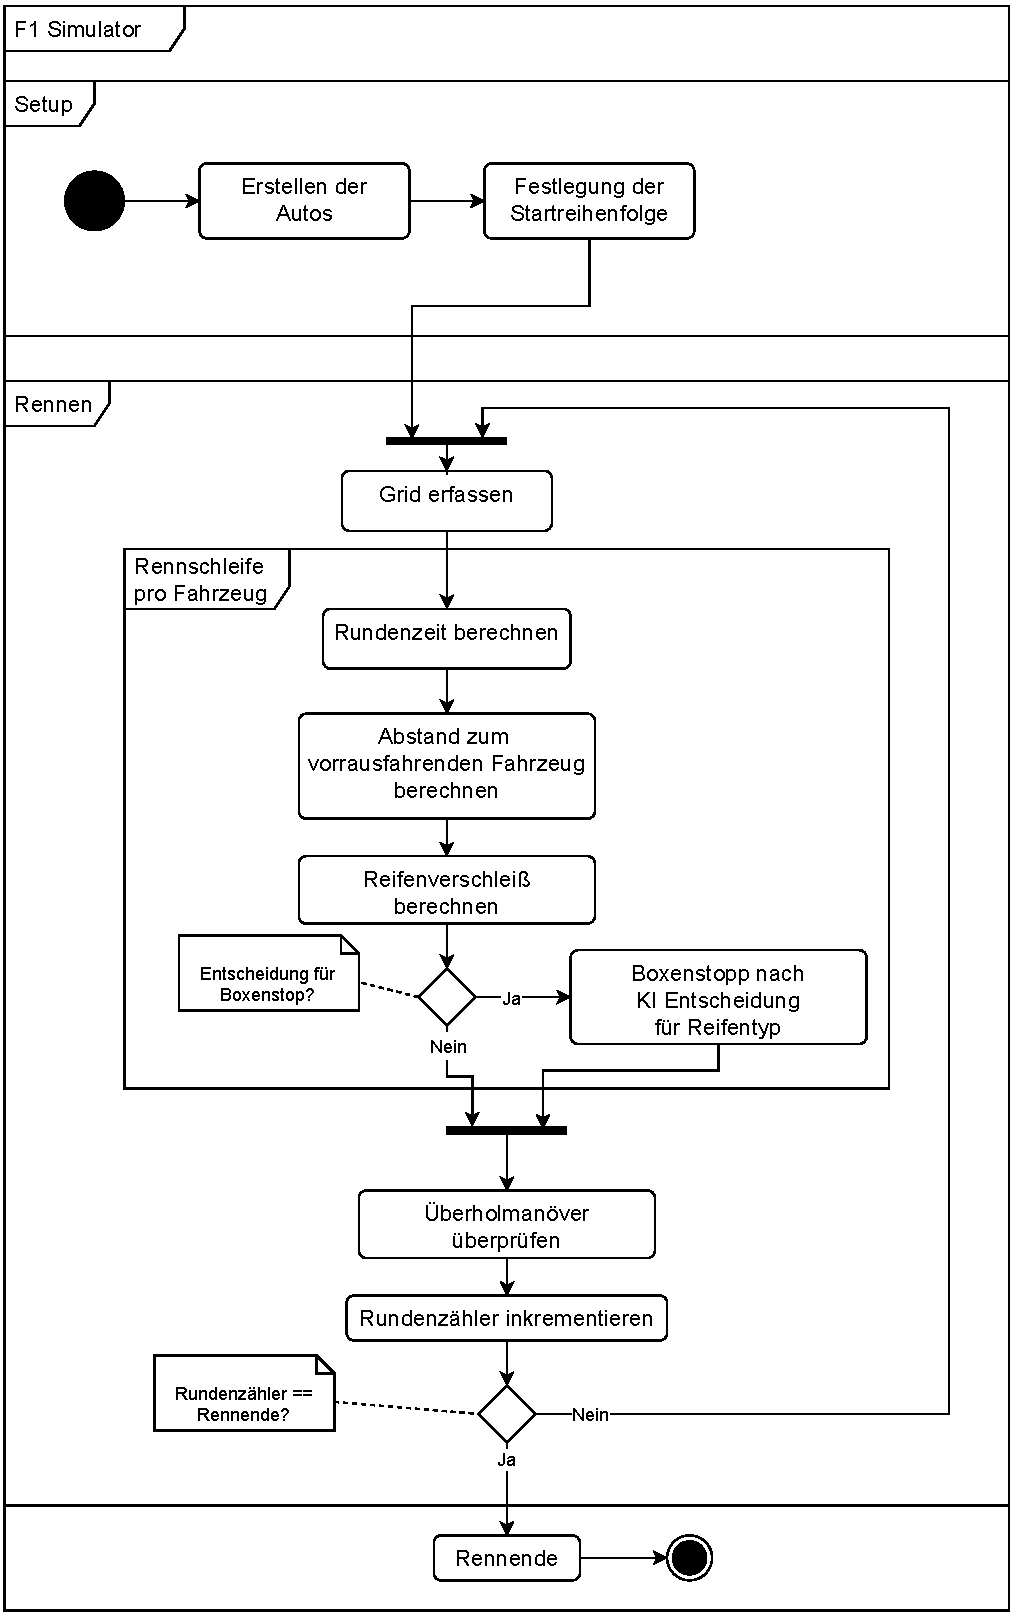
\includegraphics[scale=0.80]{Studienarbeit_F1/images/diagrams/f1_sim_architecture_overview_crop.pdf}
    \caption{Systemablaufmodell des Simulators}
    \label{fig:sim_architecture}
\end{figure}

Aus architektonischer Sicht muss besonders die angestrebte Skalierbarkeit des Simulators beachtet werden. Diese soll erlauben, zu späteren Ständen des Projektes ohne große Eingriffe und völlig ohne Umstrukturierung neue Faktoren und Funktionen in die Simulation einzubinden und somit zunehmend den Grad der Abstraktion zu reduzieren und dadurch die Aussagekraft zu erhöhen. Mit Berücksichtigung dieses Ziels wurde die grobe Architektur wie in der Abbildung \ref{fig:sim_architecture} entworfen. Dabei ist besonders die \gqq{Rennschleife} als zentraler Punkt der Architektur zu beachten, da diese so ausgelegt ist, dass jederzeit neue Funktionen eingehängt werden können und somit die Einflüsse modular erweitert werden können. Diese Architektur ist dabei an den \gqq{Single Threaded Main Event Loop} angelehnt, welcher mehrere Anfragen einzeln in einer Hauptschleife abarbeitet, dafür aber für jede eigentlich blockierende Operation einen eigenen Thread eröffnet.\cite{pattern_oriented_architecture} Den zuletzt genannten Aspekt der Generation von neuen Threads wird in unserem Ansatz nicht weiter verfolgt. Um die Modularität zusätzlich zu erreichen, werden alle Fahrzeuge sowie deren Attribute als Objekte der entsprechenden Klassen abgebildet und erlauben so den Zugriff aus jeglichen Bereichen des Systems über eine zentrale Speicheradresse der Objekte. Weiter ist die Entkopplung des Erstellens der Fahrzeuge und somit der Startaufstellung vom eigentlichen Renngeschehen zu beachten. Dies soll ermöglichen, mehrere Rennen hintereinander mit der gleichen Generation an Fahrzeugen mit gleicher Verteilung in der Startaufstellung abzubilden.

\subsubsection{Erhebung der Daten}
% Fully corrceted
% Wo kommen die Daten her und wie werden sie zielgerichtet ausgewertet? Welche Daten sind interessant?
In der Startphase des Projektes wurde auf der in \ref{sim_architecture_header} erdachten Architektur ein Prototyp erarbeitet, welcher erlaubte die Machbarkeit sowie die angestrebte Skalierbarkeit des Simulators zu prüfen. Für die Abstraktion der diversen Sachverhalte, wie beispielsweise Reifenverschleiß wurde bei dieser Grundversion aber auf die Untersuchung jeglicher Datengrundlage verzichtet, um erst einmal bei einem Prototyp zu bleiben. Nach erfolgreicher Integration einer KI in den bestehenden Prototypen wurde in der zweiten Phase des Projektes die fehlende Wissenschaftlichkeit des Simulators adressiert. Dies geschah durch die umfassende Analyse von relevanten Daten im Zielkontext, welche zunächst ausgewählt und aufbereitet wurden. Das Ziel ist hierbei: Gewährleistung der realitätsnahen Aussagekraft des Simulators zur Sicherstellung der Anwendbarkeit der resultierenden KI.
\\\\
Die nötigen Daten wurden durch die Python-Library \gqq{Fast F1} \cite{fast_f1} zur Verfügung gestellt. Diese API (Application Programming Interface) zeichnet sich besonders durch die umfangreiche Menge und einem hohen Detailgrad an Daten aus, welche historisch bis zum Jahr 2016 zurückreichen. So stehen uns jegliche Informationen auf die Runde genau von jedem einzelnen Fahrzeug zur Verfügung. Dies erlaubt somit für jeden Typen Reifen ein einzelnes und aussagekräftiges Modell zu generieren. Hierfür wurde zunächst ein Parser erstellt, welcher aus den bereitgestellten Daten die für unsere Anwendung relevanten Daten herausfiltert und diese im JSON-Format nach Rennwochenende sortiert speichert. Hierbei kann dem Parser ein beliebiges Jahr sowie eine beliebige Rennwochenende übergeben werden, deren Daten anschließend nach Reifenmischung sortiert abgelegt werden. Hierfür werden die Daten für alle drei Mischungsarten untersucht und für ein jedes Auto die verwendeten Reifen eines jeden Stints untersucht und abgespeichert. Ein Stint bezeichnet hierbei den Rennabschnitt, in welchem der Reifen gefahren wird. Heißt startet ein Fahrzeug auf der Mischung \gqq{Soft} und wechselt dann in Runde \gqq{x} auf die Mischung \gqq{Medium} so wird die Renndistanz vom Start bis Runde \gqq{x} als ein Stint bezeichnet. Anschließend können damit für jeden verwendeten Reifen die Nutzungsdauer sowie die während dieser Nutzung geleisteten Rundenzeiten analysiert werden, um die Relation zwischen möglicher Rundenzeit und dem Verschleiß des Reifens zu untersuchen. Hierbei kann bei Bedarf auch der einzelne Fahrer spezifiziert werden, um die eben beschriebene Auswertung nur im Kontext eines Fahrers zu betreiben, und somit die Varianz der diversen Fahrer und Fahrzeuge ausschließen zu können.\\
Zusätzlich bietet die \gqq{Fast F1} API bereits die Option, die Daten nach Relevanz vorzufiltern. Dies bedeutet im Kontext der Formel 1, dass alle Rundenzeiten, welche nicht aussagekräftig für die Leistung des Fahrzeuges sind, bereits ausgeklammert werden. Eine Runde in der Formel 1 verliert aus Daten-technischer Sicht dann an Bedeutung, wenn in dieser Runde kein normales Renntempo gehalten werden konnte. Dies geschieht beispielsweise im Falle eines Unfalls auf der Strecke und den zugehörigen gelben Flaggen beziehungsweise dem Einsatz des \gqq{Safety Cars} oder einem vollständigem Rennabbruch bei roter Flagge.
% Bild von quick_plotter.py als Beispiels für die eben eingeführten und erklären Konzepte!
\begin{figure}[H]
    \centering
    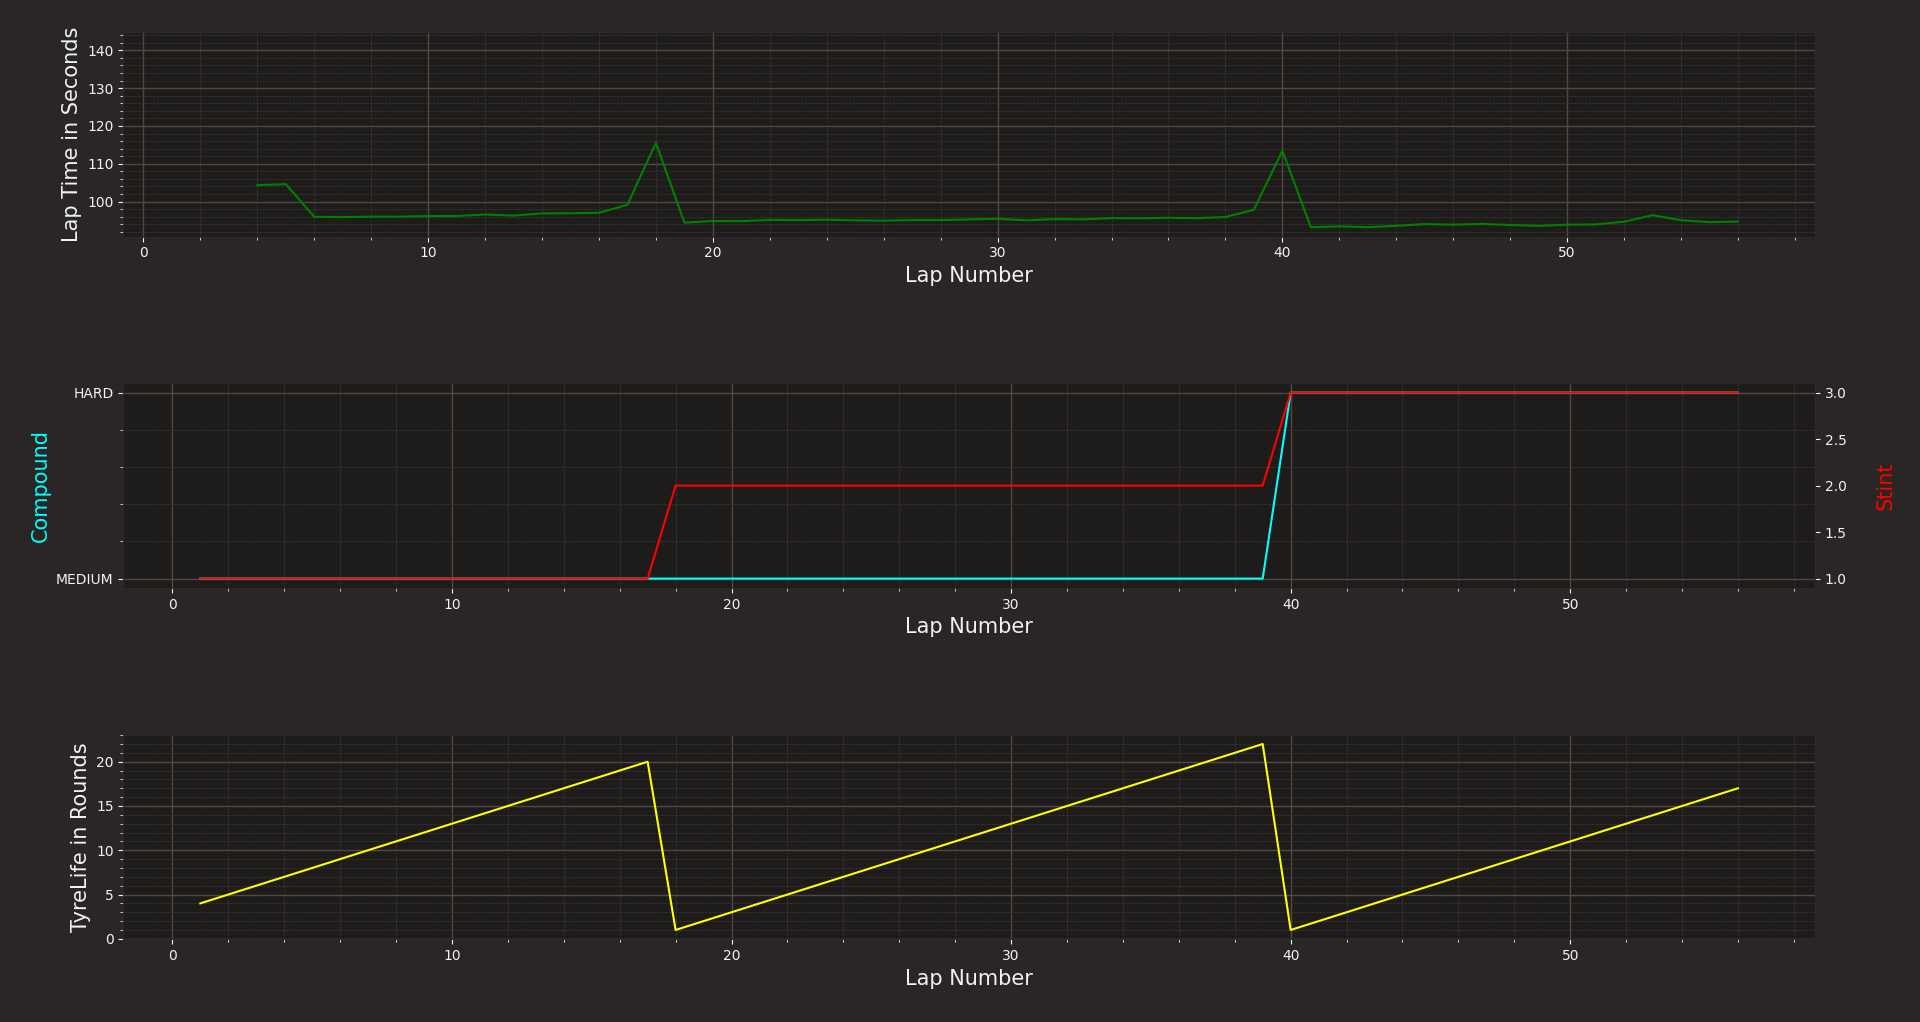
\includegraphics[scale=0.33]{Studienarbeit_F1/images/ver_race_data_example.png}
    \caption{Renndaten für Max Verstappen, Bahrain Grand Prix 2021}
    \label{fig:race_data_2021_1_VER}
\end{figure}

In Abbildung \ref{fig:race_data_2021_1_VER} ist ein beispielhafter Datensatz, welcher als Datengrundlage zur Generierung der Modelle dient, abgebildet. Hierbei sind die gefahrenen Rundenzeiten über das gesamte Rennen abgebildet, sowie die verwendeten Reifen und deren Grad der Abnutzung über die Anzahl an Runden, welche der Reifen bereits bestritten hat. Dieser Datensatz beschreibt das Rennen vom Fahrer Max Verstappen in Bahrain im Jahre 2021. Entsprechend unserer Datengrundlage können wir unsere Modelle auf die Kombination all dieser zur Verfügung stehenden Datensätze aufbauen. Über den Zeitraum von 2018 bis 2021 mit etwa 21 Rennen pro Saison und durchschnittlich 18 Autos, welche das Ziel erreichen, entspricht dies etwa 1500 nutzbare Datensätze zur Generierung der Modelle.




\subsubsection{Generierung der Modelle}\label{sec:gen_models}
% Fully corrected
% Guck ma Statistik, vllt n bissl Regression etc -> Alos von Daten zu Modellen beschreiben
Um aus der aufgebauten Datengrundlage effektiv Modelle zur Beschreibung der diversen Reifenmischungen generieren zu können, bedurfte es zunächst eine Möglichkeit, die Daten zielgerichtet auszulesen. Für diese Aufgabe wurde ein eigener \gqq{Query Handler} geschaffen, welcher es erlaubt, einzelne Teilmengen aus den gesamten Daten herauszufiltern. Dieser erlaubt wie schon beim Akquirieren der Daten nach dem gefahrenen Jahr, dem Fahrer und der Reifenmischung einzugrenzen. Zusätzlich ist in diesem Schritt aber wichtig, die gefundenen Stints nach einer Mindestlänge zu filtern, um somit nur aussagekräftige Datensätze zu erhalten. Dies bedeutet, dass beispielsweise alle Stints von \gqq{Hard} Reifen, welcher unter 10 Runden betrugen, nicht mit ausgewertet werden sollten, da dieser Zeitraum zu kurz ist, um das Verschleißverhalten daraus abzuleiten bei einer Lebensdauer des Reifen von etwa 50 Runden bei einer Rundenzeit von etwa 80 Sekunden. Die Lebensdauer des Reifens sollte hierbei nochmals in Kontext gesetzt werden. So beschreibt diese Nomenklatur nicht den Rahmen, in welchem der Reifen von einem neuwertigen Zustand übergeht zu einem Reifenplatzer. Vielmehr beschreibt die Lebensdauer das nutzbare Fenster, in welchem der Reifen im Rennbetrieb eingesetzt werden sollte. Dies bedeutet ein Reifen, welcher eine Lebensdauer von etwa 50 Runden besitzt, könnte bei Bedarf auch 20 weitere Runden durchhalten, aber in dieser Zeit werden die Rundenzeiten dramatisch schlechter und das Risiko eines Reifenplatzers steigt stetig, was in jedem Fall zu vermeiden ist. Somit bezeichnet der Begriff der Lebensdauer den Rahmen, in welchem der Reifen ein vorhersehbares und sicheres Verhalten besitzt und dabei kompetitive Rundenzeiten liefern kann.\\\\
Um eine möglichst repräsentative Auswertung für jede Art von Reifen durchzuführen, sollen alle relevanten Datensätze zu einem gültigen Modell zusammengefasst werden. Die somit ausgewählte Teilmenge der Datensätze kann nun aus verschiedensten Faktoren bestehen, welche zunächst eine Vergleichbarkeit der Daten untereinander verhindern. Grundlegend sind die Rundenzeiten meist auf verschiedenen Strecken gefahren, welche somit die Reifen in anderem Umfang strapazieren, aber auch entsprechend mehr oder weniger Zeit in Anspruch nehmen. Weitere Einflussfaktoren der Rundenzeit sind durch die Diversität der Autos selbst und das Können der einzelnen Personen am Steuer der Fahrzeuge gegeben. Um eine Vergleichbarkeit der Daten sicherzustellen, müssen die einzelnen Rundenzeiten der Stints auf eine Referenzzeit normiert werden. Dies schließt somit alle bisherigen Einflussfaktoren aus den Zeiten aus und belässt lediglich den Verlauf der Rundenzeit über den Zeitraum des Stints. Dieser Verlauf besitzt eine direkte Abhängigkeit zum Verschleiß des Reifens und kann somit als Basis des Modells genutzt werden.
\\
Methodisch erfolgt die Normierung durch die Auswahl einer einzelnen Rundenzeit im Stint, in unserem Falle die erste Runde des Stints. Im folgenden Schritt wird der Quotient aus Referenzzeit und der ausgewählten Rundenzeit berechnet und dann auf alle anderen Rundenzeiten des Stints angewendet, um diese somit einzelnen und unabhängig zu anderen Stints der Teilmenge zu normieren. 
\begin{equation}
    L_{nom} = L * \frac{L_{ref}}{L_{stint}}
\end{equation}
Die genutzte Referenzzeit wurde auf 80 Sekunden gewählt, da dies ungefähr der durchschnittlichen Rundenzeiten in der Formel 1 über eine Saison entspricht und somit anschließend in einer Rennlänge von etwa 70 Runden resultiert. Dies bietet auch den Vorteil, dass die KI später 70 Entscheidungen pro Rennen treffen muss und damit der Lernerfolg pro Rennen größer sein sollte als bei der Verwendung einer größeren Referenzrundenzeit. Die oben genannte Rennlänge in der Formel 1 beschreibt die Anzahl der Runden, welche zu absolvieren sind und abschließend etwa einer gesamten Renndauer von 90 Minuten entsprechen sollen.
\\
Anschließend wird aus jedem der gesammelten Datensätze, welche der gewünschten Teilmenge entsprechen und zu diesem Zeitpunkt normiert sind, ein Modell errechnet, welches perfekt den einzelnen Datensatz beschreibt. Die Errechnung der Modelle ist dabei auf einer Analyse über die Stintlänge von 0 bis Ende des Stints in Anzahl der Runden und der entsprechenden Rundenzeit pro Runde gegeben. Zur Approximation der Modelle wird die Polynominal Regression auf Basis des \gqq{Least Squares}-Ansatzes genutzt, welche in \ref{sub: polynominal_regression} näher beschrieben wird. Dies bedeutet, dass bei einer Menge von $x$ Daten auch $x$ Modelle generiert werden. Danach werden die einzelnen Modelle dann über die Verrechnung der einzelnen Parameter zusammengefasst, um somit ein einzelnes Modell zu generieren, welches die gewünschte Teilmenge vollständig repräsentiert. Das Zusammenfassen der einzelnen Parameter erfolgt hierbei über das arithmetische Mittel oder wahlweise dem Median. Wobei sich das arithmetische Mittel durch seine glättende Eigenschaft besser eignet.
\\\\
Das Modell zur Betrachtung der individuellen Leistung eines Fahrzeuges in Kombination mit dem Fahrer soll dabei auf der Auswertung zwischen dem schlechtesten Fahrer im schlechtesten Auto und dem besten Fahrer im besten Auto erfolgen. Hierbei ist das Kernproblem, dass der Fahrer aus den Daten heraus nicht vom Fahrzeug getrennt betrachtet werden kann, da nur zwei Fahrer im Feld das gleiche Fahrzeug besitzen. Somit kann nur eine Aussage zwischen diesen Fahrern getroffen werden. Ein Vergleich des fahrerischen Könnens über das ganze Feld hinweg ist wissenschaftlich schwer realisierbar, da die Ergebnisse der einzelnen Fahrer immer direkt mit der Leistung des Fahrzeuges korrelieren.\\
Um dennoch ein Modell zu generieren, welches uns die zeitliche Differenz pro Runde in Kontext zur Fahrzeugleistung und Fahrerleistung setzt, werden repräsentative Datensätze ausgewählt und wie beim Reifenmodell auf eine Referenzrundenzeit von 80 Sekunden normiert, um anschließend den mittleren zeitlichen Unterschied pro Runde zwischen Datensätzen verschiedener Leistung zu generieren und daraus ebenfalls mit Hilfe der Polynominal Regression ein aussagekräftiges Modell zu erstellen. Dieses soll dann die einzelnen Parameter der Leistung des Fahrzeuges und des Fahrers als Summe zu einem Zeit-Delta pro Runde korrelieren. Diese Parameter sind im Simulator als Werte zwischen $[0,1]$ gegeben mit $1$ für die beste Leistung. Entsprechend soll das Modell einem Fahrzeug, welches eine kombinierte Leistung von $2$ besitzt, keine zusätzliche Zeit pro Runde aufaddieren.


\subsection{Künstliche Intelligenz}
\label{künstliche_Intelligenz}
Auf Basis des initial entwickelten Simulators wurden die ersten Versuche der KI-gestützten Optimierung der Rennstrategie unternommen. Ziel dieser Bemühungen war es, für einen bestimmten Akteur des Rennens für jeden Zeitschritt der Simulation eine Aktion abzuleiten, die abhängig vom momentanen Rennzustand die Position des gewählten Fahrers verbessert. Diese Anforderungen resultieren in den folgenden, zu lösenden Subproblemen:
\begin{enumerate}
    \item Evaluierung von geeigneten KI-Algorithmen
    \item Integration eines Prototypen in die existierende Architektur
    \item Optimierung der KI-Parameter
    \item Evaluierung der Performance
\end{enumerate}
Im Weiteren werden die verfolgten Ansätze zur Bewältigung dieser Hürden erläutert.

\subsubsection{Evaluierung geeigneter KI-Algorithmen}
Um eine Optimierung des Renngeschehens realisieren zu können, ist es vonnöten, den Zustand einzelner Akteure in eine der vier möglichen Aktionen umzusetzen. Drei dieser Optionen beinhalten einen Pitstop mit verschiedenen Reifen, während die übrige Möglichkeit das unveränderte Fortfahren repräsentiert. Benötigt wird folglich eine Abbildung, die sowohl die Wahl des zu optimierenden Akteurs sowie alle erhältlichen Daten des Simulators als Eingabe nimmt und diejenige der 4 möglichen Handlungen, welche die Position des gewählten Akteurs optimiert, zurück gibt. Während die Größe der Eingabe- und Ausgabevektoren mittels der bereits beschriebenen Perzeptron-Technik der neuronalen Netze realisiert werden kann, ist bei der Verwendung eines solchen Ansatzes fragwürdig, inwiefern die Zuordnung des korrekten Fahrers einfach durch das Nutzen eines zusätzlichen Eingabeparameters geschehen kann. Diese Assoziation müsste aus dem Lernprozess des Netzes hervorgehen, jedoch ist keineswegs garantiert, dass solch ein Effekt auftritt. Um zu garantieren, dass diese Anforderung folglich im finalen Algorithmus realisiert wird, sollten äußere Anforderungen dieser Form nicht als durch den Lernprozess zu beseitigende Freiheitsgrade der KI repräsentiert werden, sondern nach Möglichkeit durch die architektonisch bedingten Grenzen forciert werden. Konkret bedeutet dies, dass eine Assoziation des gesteuerten Fahrers und der KI im ersten Versuch nicht mittels der Eingabeparameter geschieht.\\
Eine weitere Problematik des skizzierten Ansatzes stellt die Frage des Lernprozesses dar. Die beschriebene Technik lässt sich dem überwachten Lernen zuschreiben und benötigt für den Lernprozess die für die Anwendung \gqq{korrekten} Ausgabevektoren. Die optimalen Simulatoreingaben für die Positionsoptimierung zu jedem Zeitschritt zu ermitteln ist jedoch gerade die Motivation für die Entwicklung des Netzes, folglich greift der Ansatz des klassischen neuronalen Netzes allein für die vorliegende Problematik zu kurz und muss erweitert werden.\\
Die Behandlung der vorliegenden Problematik lässt sich vereinfachen, indem die Umgebung des Simulators als Spiel verstanden wird. Durch das Ausführen einer Aktion wirkt der Agent auf sein Umfeld ein und produziert in jeder Runde einen neuen Zustand. Am Ende des Rennens kann eine Bewertung des Spielers basierend auf seiner Position erfolgen. Es ist daher naheliegend, hier auf die existierenden Techniken beim maschinellen Lernen von einfachen Spielen zurückzugreifen. Die am weitesten verbreiteten Verfahren hierbei lassen sich unter dem Begriff \gqq{reinforcement-learning} (RL) zusammenfassen. Eine Übersicht einiger Techniken findet sich in \cite{reinforcement_learning_study}. Gemeinsames Ziel dieser Ansätze ist es, einen Lernprozess für derartige Probleme zu beschreiben, bei denen ein sogenannter \gqq{Agent} durch die Interaktion mit seiner Umgebung ein Steuersignal in Form einer Belohnung erhält, das bestimmte Verhaltensweisen fördern und andere behindern soll. \cite{reinforcement_learning_study} nennen für die Charakterisierung eines RL-Problems die folgenden beschreibenden Eigenschaften: 
 \begin{itemize}
     \item Eine diskrete Menge von Umgebungszuständen
     \item Eine diskrete Menge von vom Agenten zu tätigenden Aktionen
     \item Eine Menge von Zahlen als Belohnungen dienen
 \end{itemize}
 Um diese Punkte für den Rennsimulator herzustellen wird lediglich noch eine Funktion zur Ausschüttung von Belohnungen basierend auf dem Zustand benötigt.\\
 Die verschiedenen Ansätze des reinforcement-learning lassen das Optimieren der Leistung eines maschinellen Spielers in einer breite Klasse an Spielumgebungen zu. Beispielhaft sind Erfolge bei verschiedenen Atari-Spielen wie in \cite{atari_deep_reinforcement_learning} zu nennen oder das Meistern des komplexen Spieles Go durch Googles AlphaGo zero\footnote{\cite{alpha_go}}. Um eine für die vorliegende Anwendung zielführende Technik zu finden werden zunächst einige RL-Ansätze vor dem Hintergrund des Rennsimulators beleuchtet.


\subsubsection{Q-learning und Deep-Q-learning}
Allgemeines Ziel des Reinforcement-Learnings ist es, den Erwartungswert der kumulierten Belohnungen zu maximieren. Ein grundlegendes Modell der gesamten erhaltenen Belohnungen \(Q\) in Abhängigkeit eines Zustands \(s\) und einer Aktion \(a\) lässt sich wie folgt definieren:
\[Q(s, a) = r + Q(s')\]
Wobei \(r\) die initial ausgeschüttete Belohnung darstellt und \(Q(s')\) die gesamten zukünftigen Belohnungen ab dem nächsten Zustand bei Ausführung einer bestimmten Aktion repräsentiert. Ein Q-Learning Algorithmus lernt die Q-Werte für jedes Tupel aus Zustand und Aktion näherungsweise zu bestimmen und folglich diejenige Aktion zu ermitteln, die den Maximalwert liefert. Es resultiert ein Pfad aus Handlungen des Agents, der eine nach dem Lernprozess optimale Strategie abbildet. Abhängig von der zu erlernenden Aufgabe resultieren verschiedene Ansätze beim Schätzen des Q-Wertes in unterschiedlich effektiven Lernprozessen und Strategien. Aufgrund der inexakten Natur des von einem Algorithmus gelieferten Q-Wertes ist es opportun, die weiter in der Zukunft liegenden und damit ungenauer bestimmbaren Belohnungen weniger stark zu gewichten als solche, die mit geringer Varianz ermittelbar sind. Im Weiteren kann die mathematische Darstellung zusätzlich insofern spezifiziert werden, dass der beschriebene Algorithmus immer diejenige Aktion wählt, die im maximalen Q-Wert mündet. Diese Tatsachen lassen sich wie folgt in eine verbesserte mathematische Beschreibung umwandeln:
\[Q(s, a) = r + \gamma \cdot max(Q(s'))\]
Hierbei liegt \(\gamma\) zwischen 0 und 1 und verwirklicht die geringere Sicherheit bei entfernten Werten, wie durch das rekursive Einsetzen der Definition des Q-Wertes evident wird.\\
Die Subtypen des Q-learning unterscheiden sich explizit in der Art des Lernprozesses und damit der Bestimmung von Q. Für Probleme mit einer geringen Anzahl an diskreten Zuständen und Aktionen wird eine sogenannte \gqq{Q-Table} verwendet. Dieser Ansatz lässt sich im Wesentlichen als \gqq{Bruteforce} Methode zur Ermittlung des Wertes aller möglichen Zustandstransitionen charakterisieren und ist folglich nicht im Kontext der hier vorliegenden Vielzahl an Zuständen realisierbar.\footnote{vgl. \cite{general_Q_learning}}\\
Das in der Praxis gängige Verfahren zur Kompression der Vielzahl an vorliegenden Zustands- und Aktionstupeln ist der Einsatz eines neuronalen Netzes als prädiktionsliefernde Instanz. Konkret bedeutet dies, dass zuvor ein Netz die Belohnungen für verschiedene Zustände exemplarisch durchläuft und schlussendlich in Folge dieser Beispiele die zu erwartenden Belohnungen auch ohne die Kenntnisse über alle Zustände des Systems näherungsweise bestimmen kann. Dieses Verfahren wird als \gqq{Deep-Q-Learning} bezeichnet. Die zentrale Schwierigkeit dieses Ansatzes stellt das Trainieren des Netzes dar. Wie bereits erwähnt ist ein klassisches neuronales Netz eine Technik des überwachten Lernens, dies bedeutet, dass die Daten zum Trainieren in solch einer Form vorhanden sein müssen, dass zu jedem Beispiel der korrekte Output vorhanden sein muss. Die Eingabe des Umgebungszustandes auf die insgesamt zu erwarteten Belohnungen bei der Ausführung aller möglichen Aktionen abzubilden, ist jedoch nicht trivial. Um den Lernprozess zu ermöglichen wird für die beim Deep-Q-learning verwendeten Netze\footnote{Diese werden als \gqq{Deep-Q-Networks} (DQNs) bezeichnet} die initial bei der Zustandstransition ausgeschüttete Belohnung in Kombination mit den durch das Netz selbst berechneten, zu erwartenden Belohnungen in Folge des resultierenden Zustands verwendet, um die Performance des Netzes, also den Fehler in der Ausgabe, zu bewerten. Um dies zu verdeutlichen, wird der Lernprozess im Folgenden schrittweise illustriert:
% TODO Quellennachweise für den Algorithmus
% Ist das so verständlich oder sollte das eventuell Pseudocode sein?
\begin{enumerate}
    \item Netzinitialisierung : Zufällige Gewichte liefern anfangs für jede Eingabe zufällige Ausgaben
    \item Der Agent erhält eine Prädiktion von Belohnungen des Netzes in Form des Vektors \(Q(S)\) für den momentanen Zustand \(S\) und führt diejenige Aktion aus für die der Eintrag \(Q(S)\) maximal ist
    \item Der Agent beobachtet in Folge der getätigten Aktion \(a\) eine Belohnung \(r\) und speichert diese mit dem neuen Zustand \(S'\) und dem initial vom Netz erhaltenen Vektor an erwarteten Belohnungen ab
    \item Mithilfe von \(r\) und \(Q(S')\) wird ein Belohnungsvektor \(Q'(S)_a\) mit \gqq{korrekterem} Eintrag für die getätigte Aktion berechnet.
    \item Der Fehler aus der Abweichung von \(Q(S)\) und \(Q'(S)_a\) berechnet, wobei beide Vektoren sich lediglich im \(a\) repräsentierenden Index unterscheiden
    \item Wiederhole die Schritte ab 2. für alle Trainingsbeispiele
\end{enumerate}
Die Berechnung des korrigierten Eintrags des Belohungsvektors aus Schritt 4 geschieht wie folgt: 
\[Q(S)_a = r + \gamma \cdot max(Q(S'))\]
Die Bestimmung der Belohnungen des nächsten Zustandes geschieht demnach durch das zu trainierende Netz selbst. In jedem Lernschritt wird der betroffene Eintrag also nur durch die erhaltene Belohnung in die korrekte Richtung geführt.\footnote{vgl. \cite{atari_deep_reinforcement_learning} S.5} Um die Effektivität des Algorithmus zu steigern, betont Mnih, dass es hierbei zwei Netzwerke identischer Topologie geben muss, um die initiale Berechnung von Q-Werten und die Berechnung von den gewünschten Ziel-Q-Werten zu entkoppeln. Die Gewichte des Prädiktionsnetzes werden hierbei im Lernprozess optimiert und in einem festen Intervall auf das Zielnetzwerk kopiert.

\subsubsection{Implementierung eines DQN-Prototyps}
Um die beschriebene Technik erfolgreich umzusetzen, wurde zunächst ein Prototyp mit möglichst simplem Aufbau in die existierende Architektur des Simulators eingebettet. Ziel hierbei waren zunächst die Lauffähigkeit eines neuronalen Netzes und das sichtbare Anlernen von Belohnungen zu verifizieren und darauf folgend die Effektivität des Ansatzes bewerten zu können, um weitere Entscheidungen bei der Optimierung zu treffen.\\
Der geplante Ablauf einer Lernepisode lässt sich in Abbildung \ref{fig:race_ai_learning_episode} nachvollziehen.
\begin{figure}[ht]
    \begin{center}
        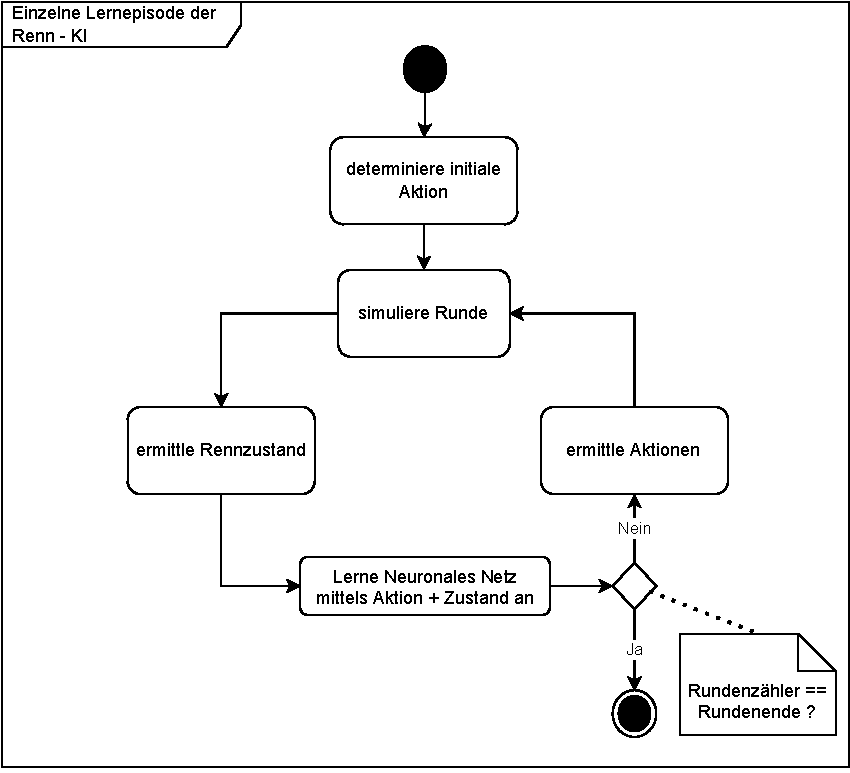
\includegraphics[]{Studienarbeit_F1/images/diagrams/race_ai_episode.pdf}
    \end{center}
    \caption{Geplanter Ablauf einer Lernepisode des DQN}
    \label{fig:race_ai_learning_episode}
\end{figure}
Einen wesentlichen Unterschied zu den bereits implementierten Funktionalitäten stellt die Rolle des Rennsimulators hier dar. Anstatt ein ganzes Rennen in einer Schleife zu simulieren, ist es für die KI-Entscheidung nötig, das Geschehen rundenweise verfolgen zu können. Opportun in diesem Kontext ist es, eine Funktion zu haben, die einen Rennzustand und die Aktionen der einzelnen Fahrer als Parameter nimmt und einen neuen Zustand zurückgibt. Der KI-Agent ist insoweit von den inneren Funktionsweisen des Simulators entkoppelt, dass verschiedene Funktionen den gesamten Rennzustand in die für das Lerngeschehen relevanten Werte umwandeln.
Explizit benötigt werden die folgenden Größen:
\begin{itemize}
    \item Die Belohnung für eine Aktion
    \item Der Eingabevektor für das neuronale Netz
\end{itemize}
In erster Iteration wurde sich bei der Eingabe des Netzes für die Anzahl der übrigen Runden bis zum Ende des Rennens, sowie die prozentuale Abnutzung des momentanen Reifens des der KI zugewiesenen Autos entschieden. Die Belohnungsfunktion besitzt zwei verschiedene Definitionen : einerseits wird für alle Runden außer der letzten eine Belohnung in Abhängigkeit der Veränderung des Abstands zum schnellsten Fahrer ausgeschüttet, andererseits wird am Ende des Rennens der finale Rückstand zum schnellsten Fahrer als negative Belohnung verteilt. Befindet sich der KI-Fahrer an erster Stelle, so wird der Abstand zum zweitschnellsten Auto zusätzlich auf die Belohnung addiert. Um die kumulierte Belohnung zu maximieren muss somit die Rundenzeit minimiert werden.\\
Die initiale Architektur des Netzes spiegelt die geforderte Simplizität des Prototypen wieder. Basierend auf dem gewählten Eingabevektor besteht die erste Schicht lediglich aus zwei Neuronen. Die Ausgabeschicht spiegelt die Anzahl der möglichen Aktionen wieder, demnach ist diese hier vier Neuronen breit. Nach Goodfellow\footnote{Vgl. \cite{goodfellow_deep_learning} S.422 f} ist die Wahl der sonstigen Hyperparameter des Netzes wie der Anzahl der Schichten und deren Größe ein problemspezifischer Prozess, der bestenfalls mittels eines bereits funktionsfähigen Prototypen durchlaufen wird. Als erste Näherung wurde sich aufgrund der geringen Komplexität der Eingabe für eine versteckte Schicht entschieden. Die Neuronenanzahl in dieser wurde mit 400 wissentlich zu hoch angesetzt, da vermutet wurde, dass die höhere Anzahl zwar zu einem langsameren Lernprozess führt, aber die zu prüfende Funktionsfähigkeit des Ansatzes trotzdem observierbar wird. Die Lernrate wurde nach ähnlicher Methode mit einem Initialwert von \(10^{-5}\) festgesetzt. Hierbei wurde vermutet, dass aufgrund der von Goodfellow betonten Wichtigkeit dieses Parameters eine Nachjustierung erfolgen müsste.\\
Weitere wichtige Entscheidungen beim Design des Netzes sind die Wahl der Aktivierungsfunktion und der Fehlerfunktion. Aus den bereits in Kapitel \ref{künstliches_neuron} beleuchteten Aktivierungsfunktionen scheint die ReLU-Funktion für die vorliegenden Eingaben und Ausgaben am besten geeignet. Die Eingabegrößen sind stets positive Zahlen mit leicht unterschiedlichen Wertebereichen und die gewünschten Ausgaben reichen von \(-\infty\) bis \(\infty\), was sich leicht durch Anwendung von ReLU in allen Schichten außer der letzten erreichen lässt. Für die finale Schicht wird als Aktivierungsfunktion die Identitätsfunktion verwendet, um auch den negativen Wertebereich abzudecken.
Als zu minimierende Kostenfunktion des Netzes wurde sich für die mittlere quadratische Abweichung des Zielwertes vom momentanen Wert der Ausgabe entschieden, da diese einen intuitiv nachvollziehbaren Zusammenhang zwischen der Netzausgabe und
dem Fehler herstellt, was die Evaluierung des Netzes durch die bessere Nachvollziehbarkeit der einzelnen Schritte vereinfacht.
Eine zusammenfassende Übersicht der initialen Konfigurationen im Weiteren relevanter Parameter als Python-Code findet sich in Listing \ref{lst:params}.
Bezüglich des Lernprozesses ist zu ergänzen, dass die Erfahrungen in Form von Tupeln aus Zustand, Aktion, Belohnung und folgendem Zustand den Erfolg des Lernens bestimmen. Um eine optimale Strategie zu entwickeln, ist es somit nötig, dem Agenten möglichst viele verschiedene Erfahrungen zukommen zu lassen.
\begin{figure}
\begin{lstlisting}[label={lst:params}, caption={Initiale Konfiguration von KI-Parametern}]
   learning_rate = 1e-5 
   gamma = 0.999
   episodes = 3000
   layer_sizes = [2,400,4]
   memory_batch_size = 500
   target_prediction_update_interval = 500
   
   # KI-Strategie
   epsilon = 1
   epsilon_decay = 0.001
   epsilon_min = 0.01
\end{lstlisting}
\end{figure}
Gleichzeitig führt eine solche Erkundung der Umgebung bei fixierten Lernepisoden dazu, dass die KI weniger Erfahrungen bei den bereits \gqq{erprobten} Strategien sammelt. Diese Balance zwischen der Erkundung neuer Strategien und der Ausnutzung derer, die nach momentanem Stand die optimale Belohnung liefert, ist als \gqq{Exploration vs. Exploitation} bekannt und muss für jedes RL-Problem gefunden werden. Um im Kontext der Renn-KI einen verbesserten Lernprozess zu provozieren, wird eine sogenannte \(\epsilon\)-greedy Policy zusammen mit Experience-Replay verwendet. \(\epsilon\)-greedy bedeutet, dass eine Variable names Epsilon verwendet wird, um die Wahrscheinlichkeit anzugeben, dass eine Aktion nicht infolge der Netzwerk-Prädiktion gewählt wird, sondern zufällig ausgeführt wird. Dieser Wert startet bei 1 und wird in jeder Episode durch den Wert von epsilon\_decay vermindert bis er einen Mindestwert erreicht. Dieses Schema ergibt eine linear abnehmende Häufigkeit an zufällig gewählten Aktionen und hilft der KI besonders in der Anfangsphase die optimale Strategie zu finden.\footnote{Vgl. \cite{deep_reinforcement_learning} S.14}\\
Experience-Replay bezeichnet das Speichern von Erfahrungen und das damit verbundene, zusätzliche Lernen aus den Selbigen. Vorteile sind die Verfügbarkeit von mehr Trainingsdaten allgemein, deren statistische Dekorrelation durch zufälliges samplen\footnote{Vgl. \cite{dqn_implementation} S.3}, sowie die Prävention von Effekten, die dem Vergessen von initialen Trainingserfolgen durch das Erfahren selektiver Trainingsdaten bei der Verfolgung einer optimalen Strategie ähneln. Ein derartiges Phänomen wird als \gqq{catastrophic forgetting} bezeichnet und kann beispielsweise durch das stetige erneute Lernen aus den früheren \gqq{Katastrophen} verhindert werden.\footnote{Vgl. \cite{experience_replay_continual_learning} S.1} Ebenso für die Mitigation dieses sich negativ auswirkenden Effektes eignet sich das alleinige Verwenden der Netzparameter, die die beste Performance liefern.

\subsubsection{Evaluierung und Anpassung des Prototypen}
Um die Funktionsfähigkeit der dargelegten Architektur zu prüfen, wurde zunächst der Lernprozess in Form von der Größe des Fehlers der Ausgabevektoren der KI und der Belohnungen zum Ende des Rennens in einem Logfile abgelegt. Hierdurch konnte schnell erkannt werden, dass der Wert der Lernrate stark reduziert werden musste. Nach einigen Episoden ergaben sich nämlich so große Werte für den Gradienten, dass die resultierenden Anpassungen der Gewichte den Wertebereich dieser überschritten, was im Log zu Einträgen mit NaN führte. Eine Lernrate von rund \(10^{-9}\) ließ diese Effekte verschwinden und lieferte nach 10 Testläufen die besten Ergebnisse verglichen mit noch kleineren Werten. Ebenfalls erkennbar wurde, dass die sehr simple Architektur mit einer hidden-Layer Schwierigkeiten hatte, die nicht stetigen Übergänge zwischen der Belohnung pro Runde und der Belohnung am Ende des Rennens zu lernen. Dies äußerte sich in Ausreißern des Fehlers am Ende jedes Rennens, welche unabhängig von der Performance der KI auftraten. Verstärkt wurden diese durch das Verwenden der mittleren quadratischen Abweichung als Fehlerfunktion, die derartige Extremwerte zusätzlich gewichtet. Grundsätzlich ist ein Auftreten großer Fehlerwerte am Ende des Rennens gewünscht, da hier der größte Lerneffekt auftreten sollte. Ein angelerntes Netz sollte derartige Sprünge jedoch nicht aufweisen. Um das Problem zu lösen, wurde zunächst der gesamte Wertebereich der Belohnungsfunktion verkleinert. Diese Änderung resultiert in einer verkleinerten Streuung der Belohnungen über die Zeit und verkleinert die Ausreißer erheblich. Jedoch musste die Lernrate infolge der nun verringerten Fehlerwerte wieder erhöht werden. Um einen effizienteren Trainingsprozess zu erreichen, wurde die Anzahl der Neuronen in der versteckten Schicht zusätzlich auf 30 reduziert, da hier keine Verschlechterung wahrgenommen werden konnte. Mit diesen Änderungen gelang es, einen KI-Agent zu trainieren, der sichtliche Lernerfolge erzielt und zuverlässig eine bessere Platzierung als die initiale, untrainierte KI erreichen kann. Die Abbildungen \ref{fig:AI_initially_trained_soft} und \ref{fig:AI_initially_trained_hard} zeigen diesen Lernfortschritt in Form der gesammelten Belohnungen am Ende des Rennens nach den durchlaufenen Episoden für zwei Durchläufe bei identischer Konfiguration.
Auffallend bei Abbildung \ref{fig:AI_initially_trained_soft} ist, dass die KI nach einer anfänglichen Einfindungsphase in ein oszillierendes Schema von Strategiewechseln verfällt. Das Muster resultiert daraus, dass die KI lernt, dass ein besseres Ergebnis dadurch erzielt werden kann, einen Reifen weniger oft zu wechseln. Folglich nähert sich die Lebenszeit des Reifens immer mehr den 0\%, ab welchen die Rundenzeit stark zu steigen beginnt. Dies führt zu einem großen Fehler in der Schätzung des neuronalen Netzes und demnach auch in einer großen Anpassung der Gewichte. Die vorherige Strategie wird damit als schlechter bewertet und der Agent weicht auf diejenigen Aktionen aus, die nun die besten Belohnungen liefern. Diese neue Strategie liefert im Mittel jedoch schlechtere Resultate als die Alte, somit kehrt der Agent nach einigen Episoden wieder zur Ausgangsstrategie zurück.
\begin{figure}
\begin{center}
    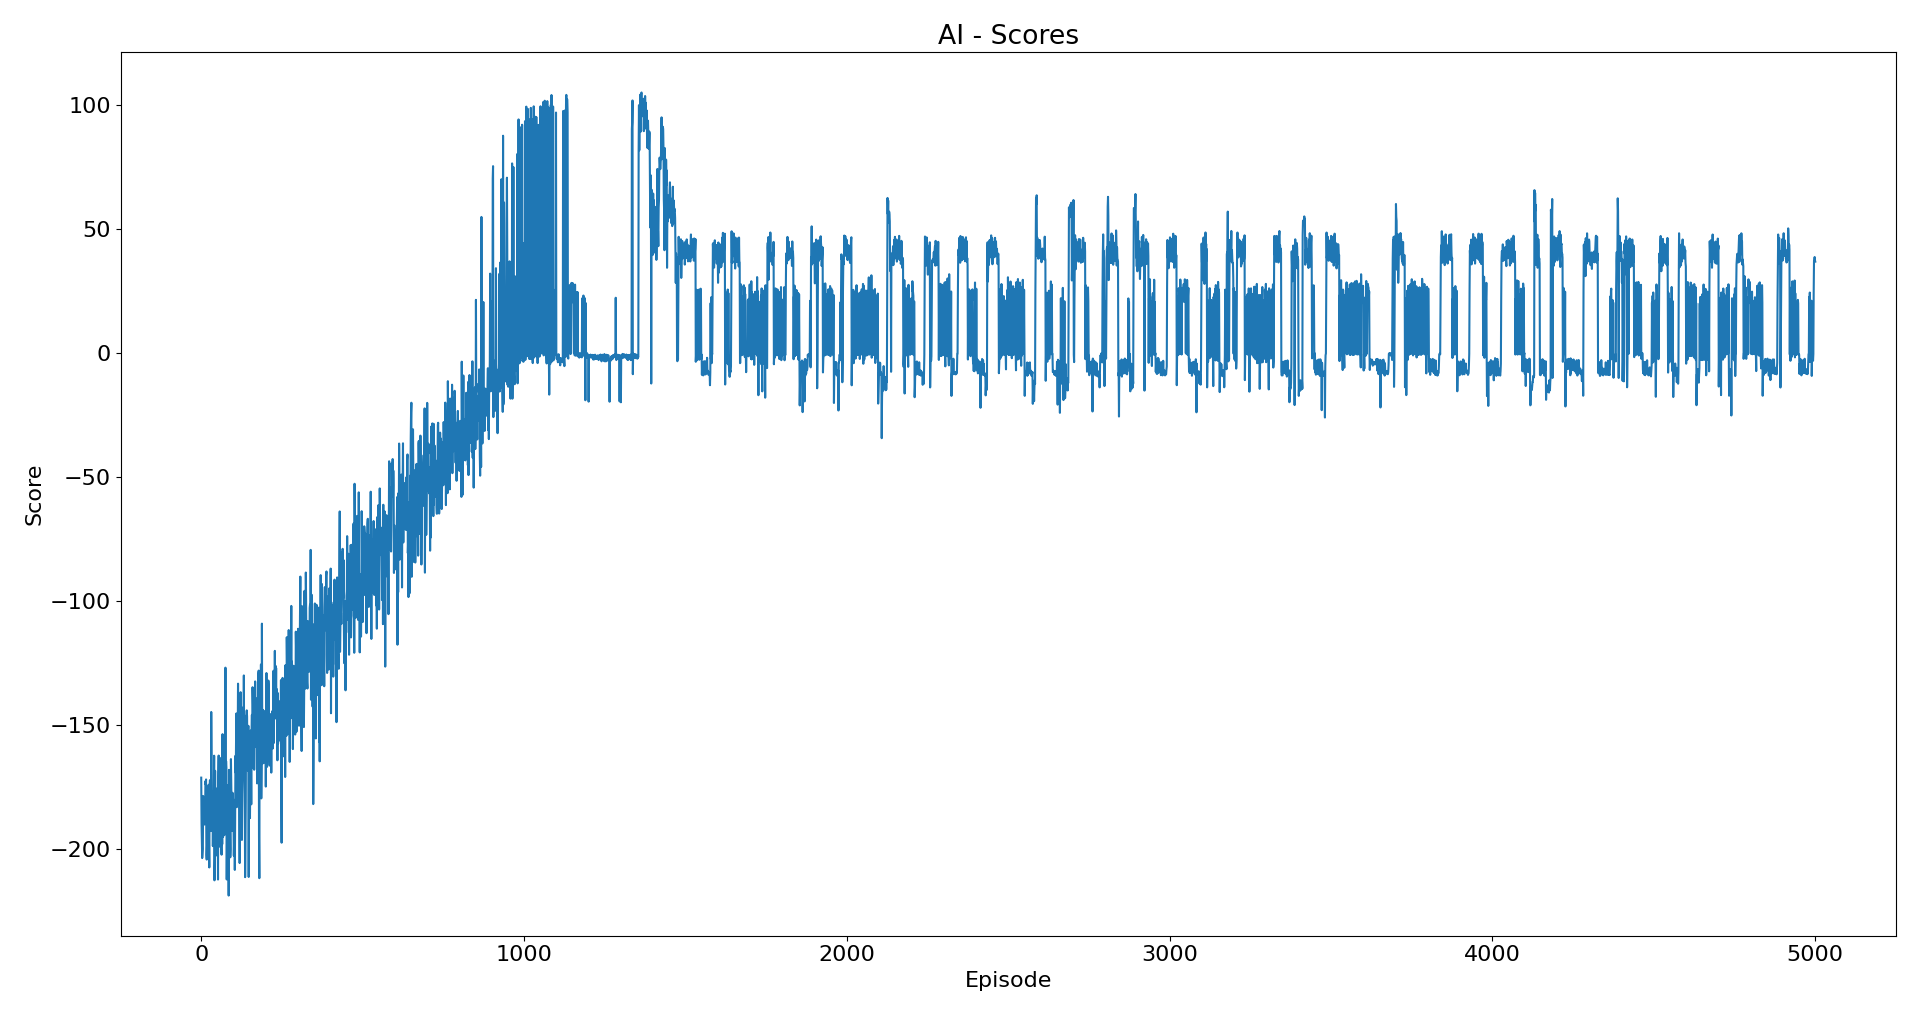
\includegraphics[scale=0.33]{Studienarbeit_F1/images/scores_5000eps_soft.png}
    \caption{Summierte Belohnungen nach jeder Lernepisode über 5000 Episoden. Eine Lernepisode repräsentiert ein Rennen mit 70 Runden. Die ersten 1000 Episoden werden durch die Epsilon-Policy dominiert.}
    \label{fig:AI_initially_trained_soft}
\end{center}
\end{figure}
\begin{figure}
    \centering
    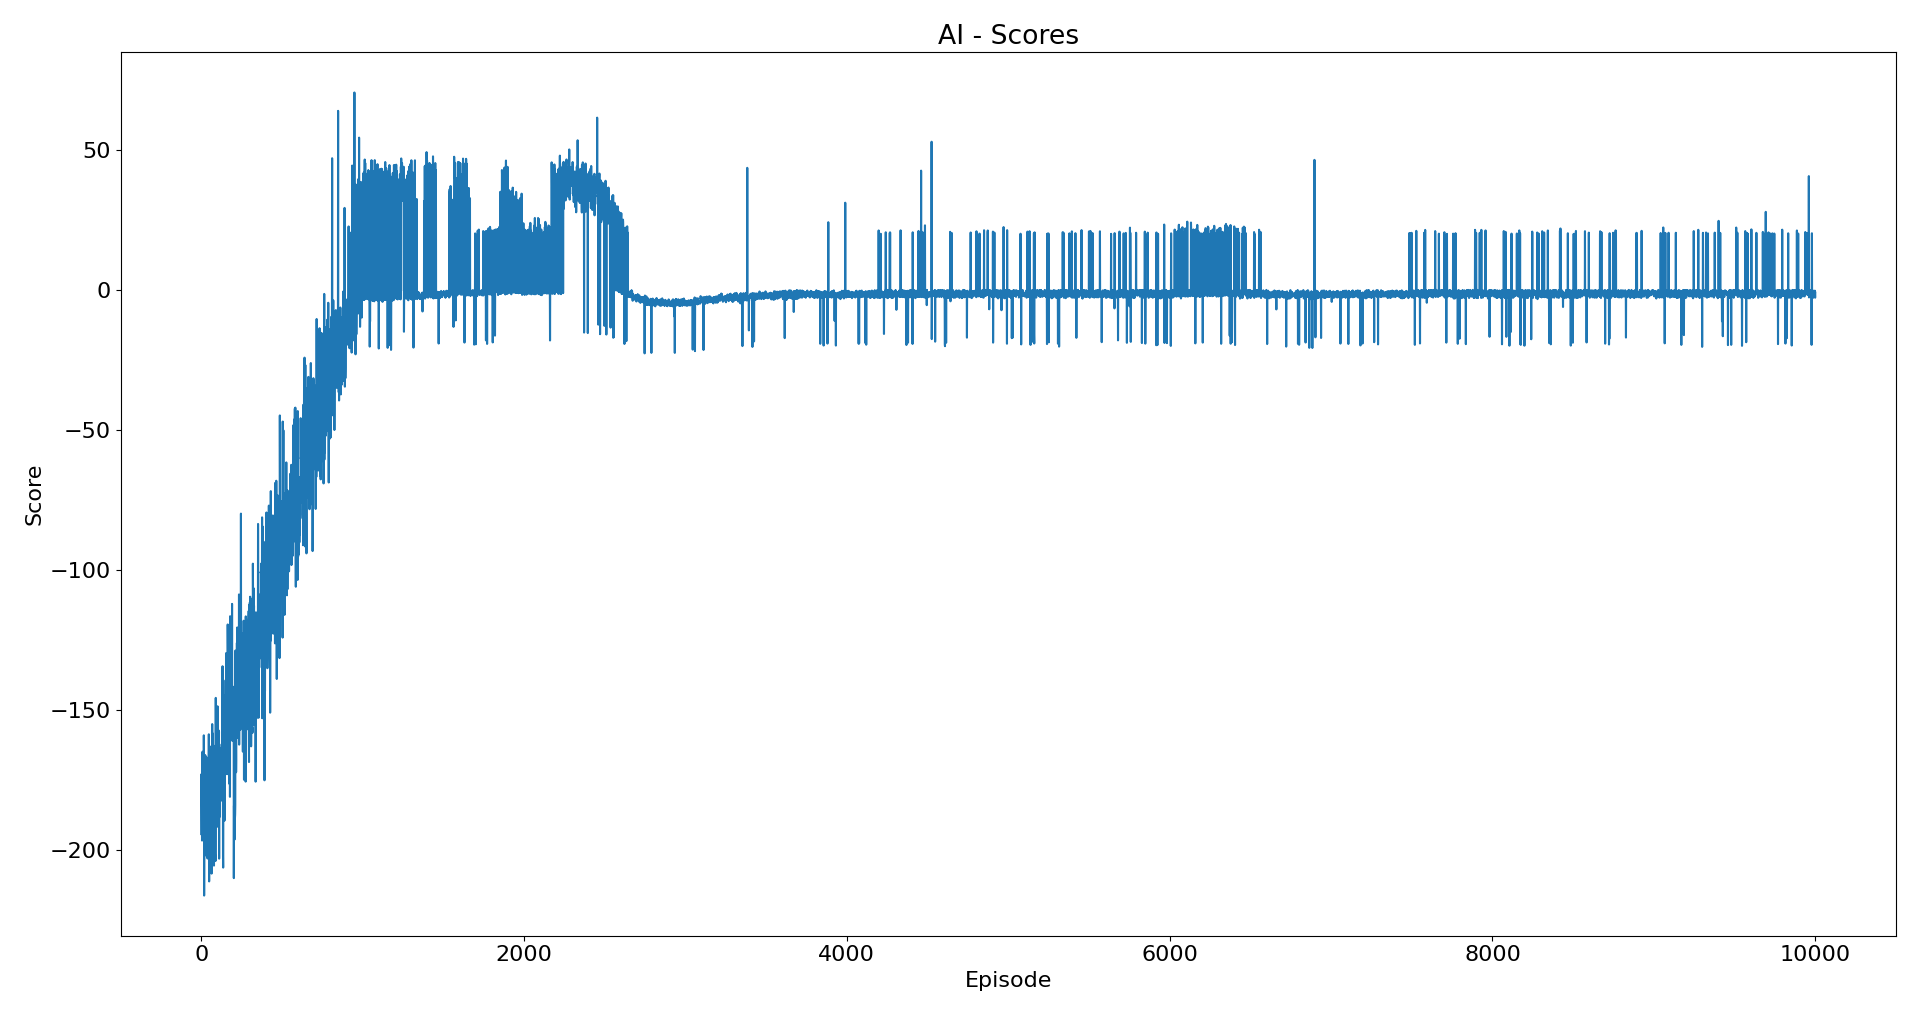
\includegraphics[scale=0.33]{Studienarbeit_F1/images/scores_10000eps_hard.png}
    \caption{Summierte Belohnungen nach jeder Lernepisode über 10000 Episoden. Es dominiert bei gleicher Konfiguration wie in Abbildung \ref{fig:AI_initially_trained_soft} eine unterschiedliche Strategie.}
    \label{fig:AI_initially_trained_hard}
\end{figure}
Zusätzlich für einen suboptimalen Lernprozess spricht der im Vergleich in Abbildung \ref{fig:AI_initially_trained_hard} gezeigte Verlauf. Bei einer idealen Erkundungsstrategie des Agenten ist zu erwarten, dass jeder Trainingslauf bis auf geringe Unterschiede diejenige Strategie hervorbringt, die die optimalen Resultate erzielt. Es folgt, dass der hier verfolgte Ansatz nicht die optimalen Lösungen erzielt. Zudem deuten die Unterschiede im Lernprozess kurz nach der Exploration-Phase zu denen zum Ende des Trainingsprozesses darauf hin, dass die durch den KI-Agenten gesammelten Erfahrungen in den beiden Zeiträumen in zu großer Weise unterschiedliche Probleme repräsentieren. Für das Erzielen einer optimalen Strategie wurden somit zusätzliche Änderungen an den Parametern ausprobiert. Weiteres Variieren der Hyperparameter, das Evaluieren verschiedener Experience-Replay Parameter, das Erhöhen der Anzahl der hidden-Layer, sowie die Tests mit größeren Episodenlängen und Erkundungsperioden lieferten vergleichbare, suboptimale Verläufe. Um den Lernprozess zu verbessern, wurde somit versucht, sowohl den Lernalgorithmus als auch die Zusammenstellung der Datengrundlage in Form des Speichers für Experience-Replay zu optimieren.
Zunächst wurden die existierenden Verbesserungen des DQN-Algorithmus aus \cite{rainbow_dqn} betrachtet. Ziel war es, auszuschließen, dass die unerwartete Entwicklung des Lernvorgangs aus der Implementierung des instabilen DQN-Algorithmus hervorgeht, dessen Performance durch einige teilweise sehr simple Änderungen, optimiert werden kann. Die wohl naheliegendste Verbesserung stellt das Verwenden eines \gqq{double-DQN} nach \cite{double_q_learning} dar. Dieser verändert den Algorithmus insoweit, dass die für die Bestimmung des Ziel-Q-Wertes benötigte Bewertung des Folgezustandes nach Tätigung einer Aktion entkoppelt wird. Anstatt den Zustand an das Zielnetzwerk zu geben und den Maximalwert der Ausgabe zu nehmen, wird hier zuvor die beste zu treffende Aktion durch das Prädiktionsnetz ermittelt, der Wert dieser Aktion wird jedoch durch das Zielnetz bestimmt. Diese Trennung soll der in sonstigen Fällen auftretenden Überschätzung der Belohnungswerte entgegenwirken.\footnote{Vgl. \cite{double_q_learning} S.2f}
Ebenso vielversprechend schien die Implementierung des dueling DQN nach \cite{dueling_network_architectures}. Hierbei wird die Entkopplung insofern weitergeführt, dass zwei separate Netze für die Bewertung von Zuständen und Aktionen verwendet werden. Der Q-Wert aller Aktionen ergibt sich also, indem der Eingabezustand an beide Netze gegeben wird und der Wert des Zustandes mit den Werten der Aktionen addiert wird. Praktisch müssen bei diesem Ansatz einige Details beachtet werden, um zu garantieren, dass die einzelnen Netze auch wirklich den Zustand und die Aktionen bewerten und nicht nur zufällig bei der Addition den korrekten Q-Wert liefern.\footnote{Vgl. \cite{dueling_network_architectures} S.4f}
Nach der Implementierung beider Maßnahmen konnten keine wesentlichen Unterschiede zum bereits existierenden simplen DQN bezüglich des Lernerfolges erkannt werden. Demnach wurde sich im Folgenden auf die Verbesserung der Datenbasis und die Erkundungsstrategie des Agenten konzentriert. Hierfür wurde zunächst die bisher verwendete \(\epsilon\)-greedy-Aktionsselektion durch eine Boltzmann-Verteilung ersetzt. Diese nutzt die in Kapitel \ref{künstliches_neuron} vorgestellte Softmax-Funktion um die vom neuronalen Netz gelieferten Q-Werte in eine Wahrscheinlichkeitsverteilung umzuwandeln, wobei diejenigen Aktionen, die hohe Q-Werte liefern, eine höhere Wahrscheinlichkeit besitzen, selektiert zu werden. Für das vorliegende Problem lieferte diese Art der Aktionswahl keine opportunen Ergebnisse, da die Abwesenheit der zufälligen Wahl von Aktionen am Anfang des Rennens darin mündet, dass der initiale, untrainierte Zustand der KI erheblichen Einfluss auf die gefundene Strategie hat. Eine Kombination dieser Strategie mit dem zuvor genutzten Ansatz wurde ebenfalls getestet und lieferte abhängig von den Parametern der Softmax-Distribution Ergebnisse, die entweder identisch mit denen einer reinen \(\epsilon\)-Policy waren oder denen einer reinen Boltzmann-Policy waren. Der eigentlich gewünschte Effekt der Verfeinerung der Strategie in Form des Findens des optimalen Reifentyps infolge der ähnlichen Q-Werte der Pitstop-Optionen nach der initialen, durch die \(\epsilon\)-Policy bestimmten Exploration konnte nicht beobachtet werden.\\
Aufgrund der Wirkungslosigkeit der evaluierten Maßnahmen wurden im Weiteren potentielle Fehler in der Konzeptionierung des Lernprozesses in Form der Ausschüttung von Belohnungen untersucht. Die bisherige Funktion hierfür belohnte in jeder Runde eine Verkleinerung des Abstandes zum führenden Fahrer. Dies liefert in den Runden, in denen der bestplazierte Fahrer einen Pitstop durchführt, eine positive Belohnung für die KI, ohne die Geschehnisse direkt bei der KI mit einzubeziehen, was sich negativ auf die Entwicklung einer guten Strategie auswirken könnte. Um also derartige Effekte zu verhindern, wurde die Belohnungsausschüttung insoweit verändert, dass jede Runde eine Evaluierung der Performance in Abhängigkeit der hinzugewonnenen oder verlorenen Plätze geschieht. Um weiterhin eine möglichst schnelle Rundenzeit zu provozieren, wird für den Fall, dass der Agent zum Ende des Rennens den ersten Platz belegt, zusätzlich der Abstand zum zweitplatzierten Fahrer belohnt. Die geschilderten Probleme wurden durch diese Änderung ebenfalls nicht gelöst.\\
Einen signifikanten Sprung in der Effektivität der gefundenen Strategien lieferte schlussendlich die Verwendung einer höheren Lernrate in Verbindung mit einer anderen Optimierungsfunktion. Bisher verwendet wurde die PyTorch Funktion \gqq{SGD}, was für \gqq{stochastic gradient descent} steht. Über die nun verwendete Funktion namens \gqq{Adam} schreiben die Autoren des ursprünglichen Artikels zu dessen Umsetzung folgendes: \gqq{The method is also appropriate for non-stationary objectives and problems with very noisy and/or sparse gradients}.\footnote{Vgl. \cite{adam_optimizer} S.1} Da das vorliegende Problem nicht stationärer Natur ist und die Rundenzeiten in einem gewissem Maße zufallsbasiert sind, ergibt die Verwendung dieses Optimierungsverfahrens hier Sinn.\\
Auf weitere Experimente mit dem minimalistischen Prototyp wurde an dieser Stelle verzichtet, da die Ergebnisse mit dem verbesserten Optimierungssystem als stabil genug für die Erweiterung zur Verarbeitung des gesamten Rennzustandes bewertet wurden. Stabil bedeutet in diesem Kontext, dass verschiedene Trainingsläufe ähnliche Ergebnisse liefern und die Kurve der gesammelten Belohnungen in Abhängigkeit der Lernepisode in einem bestimmten Zeitfenster näherungsweise monoton steigend ist.
Als Zwischenfazit des Testprozesses für den Prototyp des DQN-Algorithmus und dessen Verbesserungen lassen sich folgende Erkenntnisse festhalten :
\begin{itemize}
    \item Mittels des DQN-Algorithmus ist es möglich eine KI zu trainieren, die signifikante Erfolge bei der Entwicklung einer effektiven Rennstrategie erzielt
    \item Beim Trainieren der KI kann nicht davon ausgegangen werden, dass eine längere Trainingszeit zu einer besseren Performance oder zu null konvergierenden Fehlerwerten beim neuronalen Netz führt
    \item Auch bei korrekter Implementierung des Algorithmus ist eine große Menge an Testläufen für die Optimierung der Vielzahl an Parametern nötig, da diese erheblichen Einfluss auf die Qualität der erlernten Strategien hat und es keine allgemein zielführenden Verfahren zur Initialisierung dieser Parameter gibt
\end{itemize}


	\section{Ergebnisse}\label{sec:results}
% Fully corrected!
In den nachfolgenden Kapiteln werden die verschiedenen Resultate der Arbeit dargestellt und bereits die Leistung der KI in diversen Situationen abgebildet. Diese Untersuchung der Ergebnisse bietet eine wissenschaftliche Grundlage zur Identifikation der Schwachstellen der gewählten Modelle in der anschließenden Diskussion.

\subsection{Simulationsumgebung}
% Fully corrected!
Die erstellte Simulationsumgebung bietet abschließend die Möglichkeit Formel 1 Rennen auf Basis diverser Modelle zu generieren. Dabei wurden die Modelle durch Auswertung echter Renndaten erstellt und validiert. Die simulierten Rennen erlauben die Möglichkeit, die erforderliche Rundenzahl sowie die Anzahl der teilnehmenden Fahrzeuge frei zu wählen. Hierbei muss beachtet werden, dass die Referenzrundenzeit nicht einstellbar ist, da diese grundlegend in den diversen Modellen durch die Normierung der einzelnen untersuchten Stints auf die Referenzzeit von 80 Sekunden eingearbeitet wurde.
\\
Zusätzlich wurden umfassende Logging-Mechanismen zur Auswertung des aktuellen Verhaltens eines jeden Fahrzeuges in den Simulator integriert, um damit die Leistung des Simulators zu untersuchen, aber auch das Verhalten der KI in Relation zum restlichen Fahrerfeld untersuchen zu können.
\\
Zusammenfassend erfüllt der Simulator unsere Anforderungen und erlaubt somit das Training und die Validierung einer entsprechenden KI für Rennstrategie in der Formel 1. Grundlegend ist dabei die Entwicklung des Simulators aber nicht abgeschlossen, da jederzeit die angewandten Modelle hinterfragt und angepasst werden können und zudem die betrachteten Einflussfaktoren ausgeweitet werden könnten wie beispielsweise durch eine Untersuchung der Reifentemperatur.
\\\\
Die verschiedenen Modelle und deren Entwicklungshistorie werden im Folgenden dargestellt und erläutert. 

\subsubsection{Reifen Modelle}
% Fully corrected!
Die Reifen Modelle als zentraler Bestandteil unserer Simulation entstanden methodisch wie in \ref{sec:gen_models} beschrieben.\\
Die erste Iteration der gefundenen Modelle wies sich leider als fehlerhaft in der Methodik heraus und stellte keine realistische Abbildung des Reifenverhaltens dar. Diese Modelle wurden entsprechend nach der ersten Auswertung mit der KI als fehlerhaft erkannt. So repräsentierten diese Modelle einen einzelnen Fall eines Stints, zu sehen in Abbildung \ref{fig:tyre_model_single_stint} und nicht wie geplant die vollständige Auswertung über alle Stints, welche eine mindeste Anzahl an Runden beschrieben.
\begin{figure}[H]
    \centering
    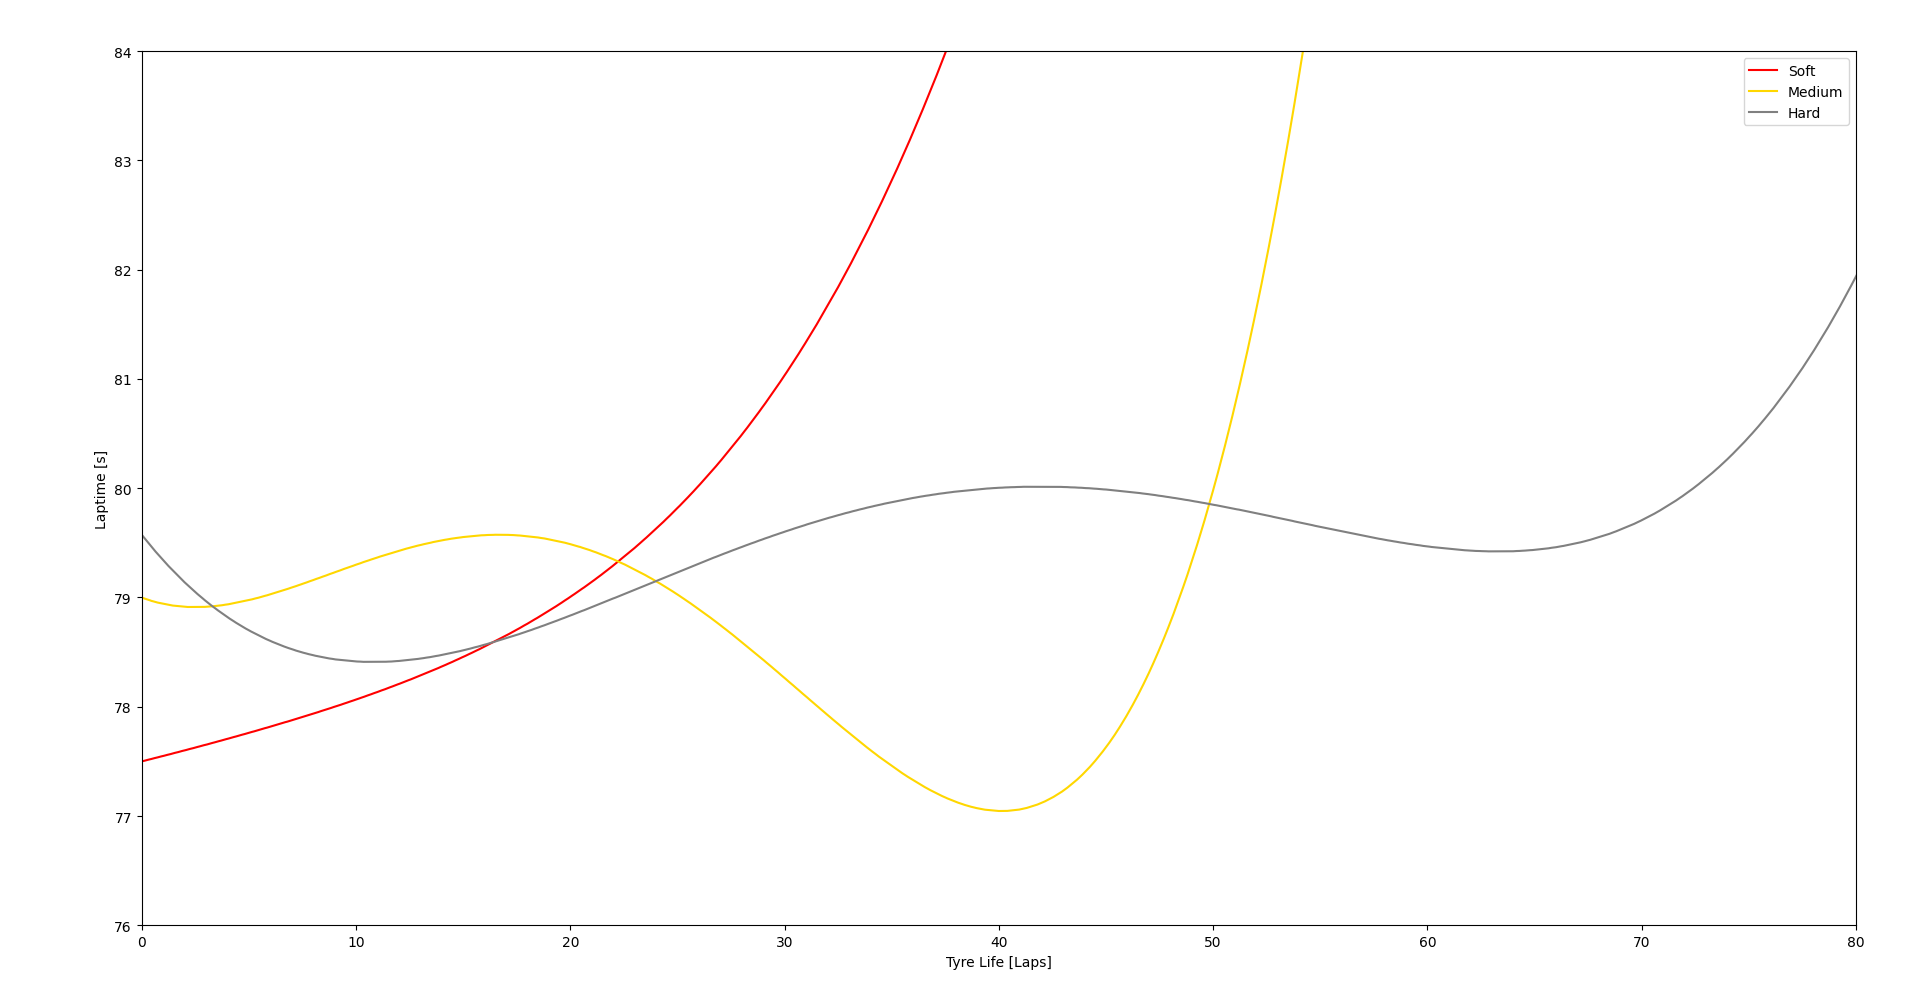
\includegraphics[scale=0.33]{Studienarbeit_F1/images/Tyre_models_better.png}
    \caption{Reifenverschleiß Modell über einen einzelnen Stint}
    \label{fig:tyre_model_single_stint}
\end{figure}
Dieses Modell ist entsprechend nicht repräsentativ und weißt sich besonders durch die starken Schwankungen über die Zeit des Stints aus. Diese sind einzelne Beobachtungen, welche nicht aussagekräftig für eine allgemeine Beschreibung des Reifens im Kontext eines allgemeinen Fahrzeuges sind. Dieses Modell ist im Kern problematisch aufgrund von sehr ausgeweiteten Stintlängen, welche beispielsweise den Soft mit einem Vorteil von bis zu zwei Sekunden pro Runde und einem kompetitiven Fenster von bis zu 35 Runden viel zu schnell abbilden .\\
Hierbei wurde in der Auswertung der Fehler gemacht, nur nach Stints zu filtern, welche mindestens eine gewisse Anzahl an Runden lang waren. Entsprechend wurden aber die statistischen Ausreißer nach oben weiterhin berücksichtigt und diese Einzelfälle, in welchen der Soft beispielsweise tatsächlich diese Leistungen erbracht hat, übermäßig berücksichtigt. Dies basierte auf der falschen Annahme, dass ein Stint umso länger dieser ist, repräsentativer für das Verhalten des Reifens wird. Grundlegend ist diese Annahme auch korrekt, da besonders kurze Stints wenig bis keine Aussage über den Verschleiß haben. Dennoch sollte für die Suche nach einem repräsentativen und realistischen Modell der Untersuchungsbereich nach oben hin limitiert sein, um nicht durch Ausreißer nach oben verfälscht zu werden. Dadurch werden Ausreißer in dieser Form nicht im Simulator auftreten können, was wiederum eine zusätzlich Abstraktion zur Wirklichkeit darstellt.
\\\\
Entsprechend dieser Beobachtung konnten die Auswertungen der einzelnen Reifenmodelle überarbeitet und korrektere Modelle aus dem Daten extrahiert werden. Diese Modelle, dargestellt in Abbildung \ref{fig:tyre_models_new}, beschreiben nun einen deutlich aussagekräftigeren Unterschied zwischen den einzelnen Reifentypen. Besonders gut zu sehen ist der lineare Verlauf des Verlusts an Gewicht in den Fahrzeugen, welches es erlaubt, über den Stint hinweg zunehmend schneller zu fahren, trotz des Verschleißes des Reifens. Mit Ende der Lebenszeit des Reifens, wie in \ref{sec:gen_models} beschrieben, greift aber dennoch der Verschleiß des Reifens und dieser baut zunehmend an Leistungspotential ab.\\
\begin{figure}
    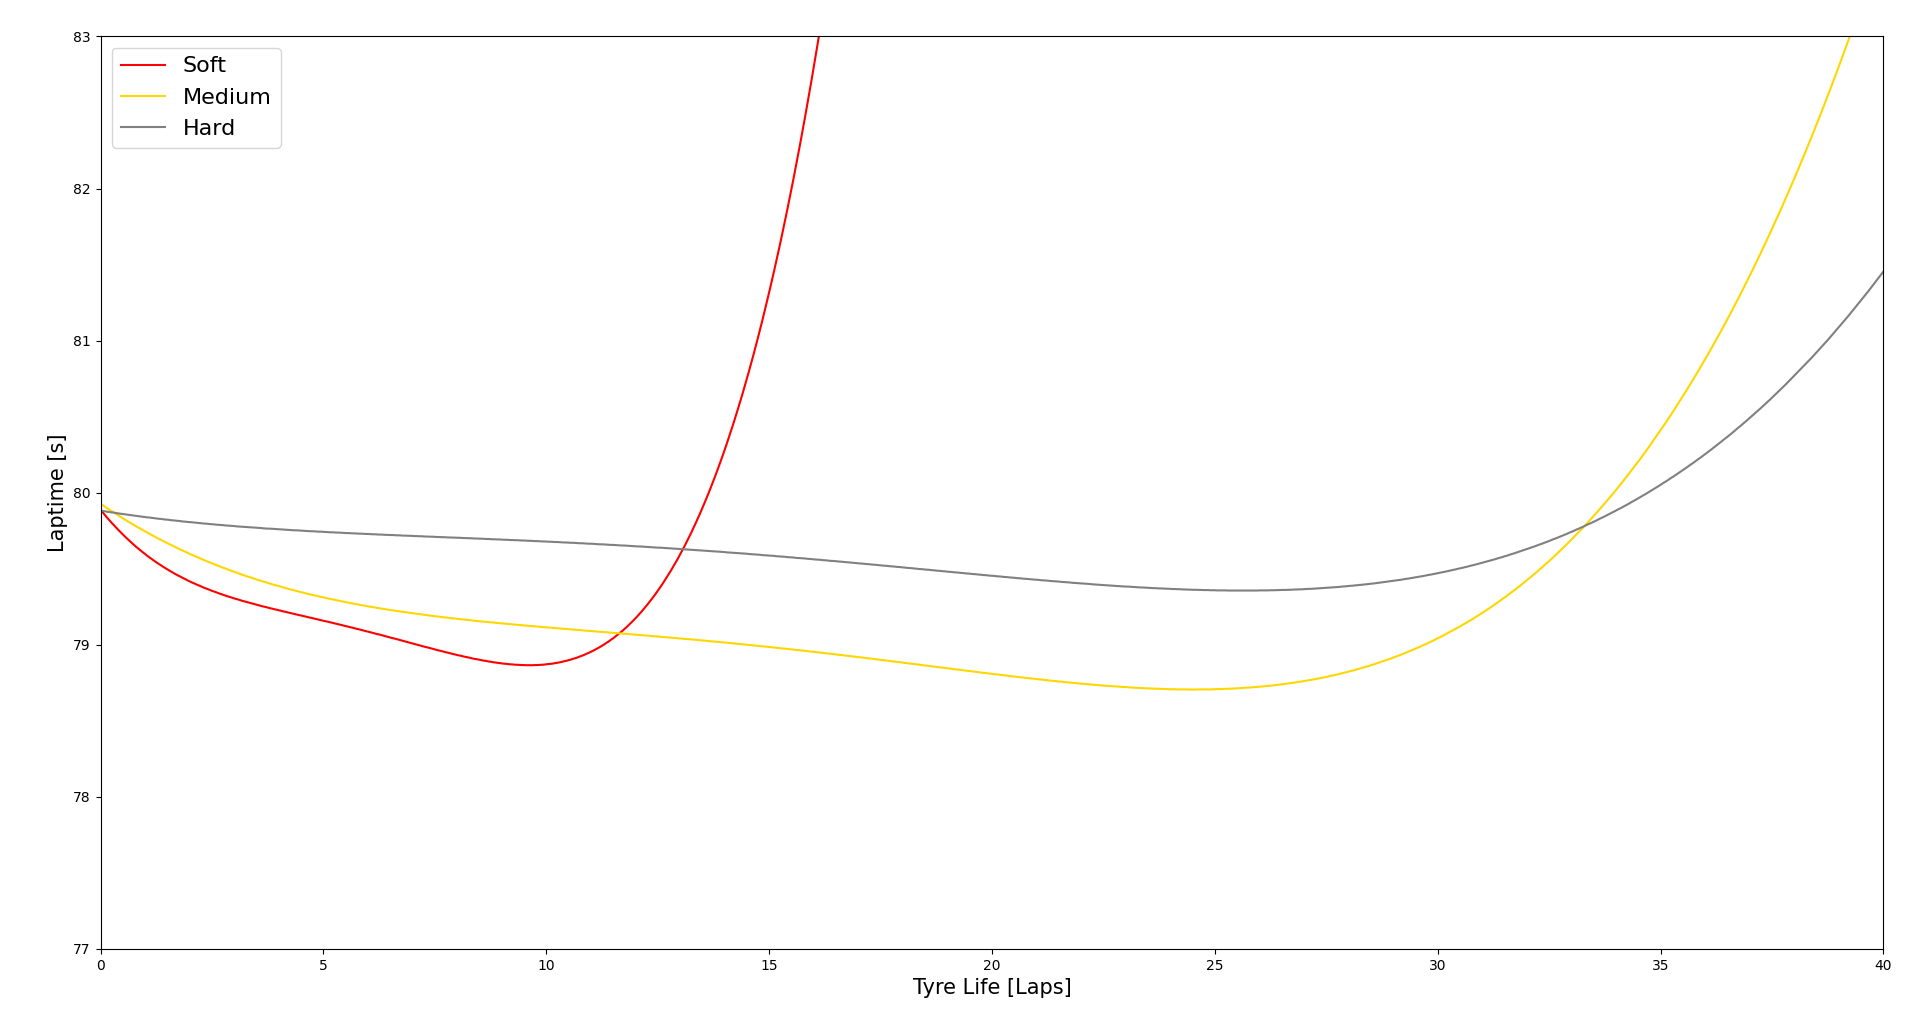
\includegraphics[scale=0.33]{Studienarbeit_F1/images/tyre_models_new_size.png}
    \caption{Abschließende Reifen Modelle}
    \label{fig:tyre_models_new}
\end{figure}

\subsubsection{Individuelles Leistungsmodell}
% Fully corrected!
Das individuelle Leistungsmodell soll, wie bereits in \ref{sec:gen_models}, den Leistungsparameter, welcher im Simulator durch einen Wert zwischen $[0,1]$ beschrieben ist, eines einzelnen Fahrzeuges in Kombination mit dem Fahrer auf den entsprechenden Zeitverlust pro Runde abbilden. Der Leistungsparameter des Fahrers ist ebenfalls im Intervall $[0,1]$ definiert. Entsprechend soll der beste Fahrer im besten Auto keine weitere Zeit auf seine Rundenzeit addiert bekommen, während der schlechteste Fahrer im schlechtesten Fahrzeug das maximale Zeitdelta erhält.\\
Aufgrund der Tatsache, dass die Leistung eines Fahrers direkt mit der Leistung des Fahrzeuges zusammenhängt, kann eine Auswertung und ein resultierendes Modell nicht mit einer solchen Genauigkeit die einzelnen Parameter direkt abbilden. Somit muss das gesuchte Modell die Leistung des Fahrzeuges und die Leistung des Fahrers kombiniert betrachten. Dadurch wird das gesuchte Modell im Intervall von $[0,2]$ die Zeitdifferenz pro Runde für ein Fahrzeug mit Fahrer abbilden.\\
Für diese Auswertung wurde die Saison 2021 betrachtet. Hierfür wurden die Zeiten der schlechtesten Kombination von Fahrer und Fahrzeug, was in diesem Fall dem russischen Piloten Nikita Mazepin des Teams \gqq{Haas F1} entspricht, mit der besten Kombination von Fahrer und Fahrzeug auf die mittlere Differenz der Rundenzeiten untersucht. Als optimal Fall wurde der britische Fahrer Lewis Hamilton im Mercedes betrachtet. Resultat dieser Auswertung ist das Modell in Abbildung \ref{fig:individual_model}.
\begin{figure}
    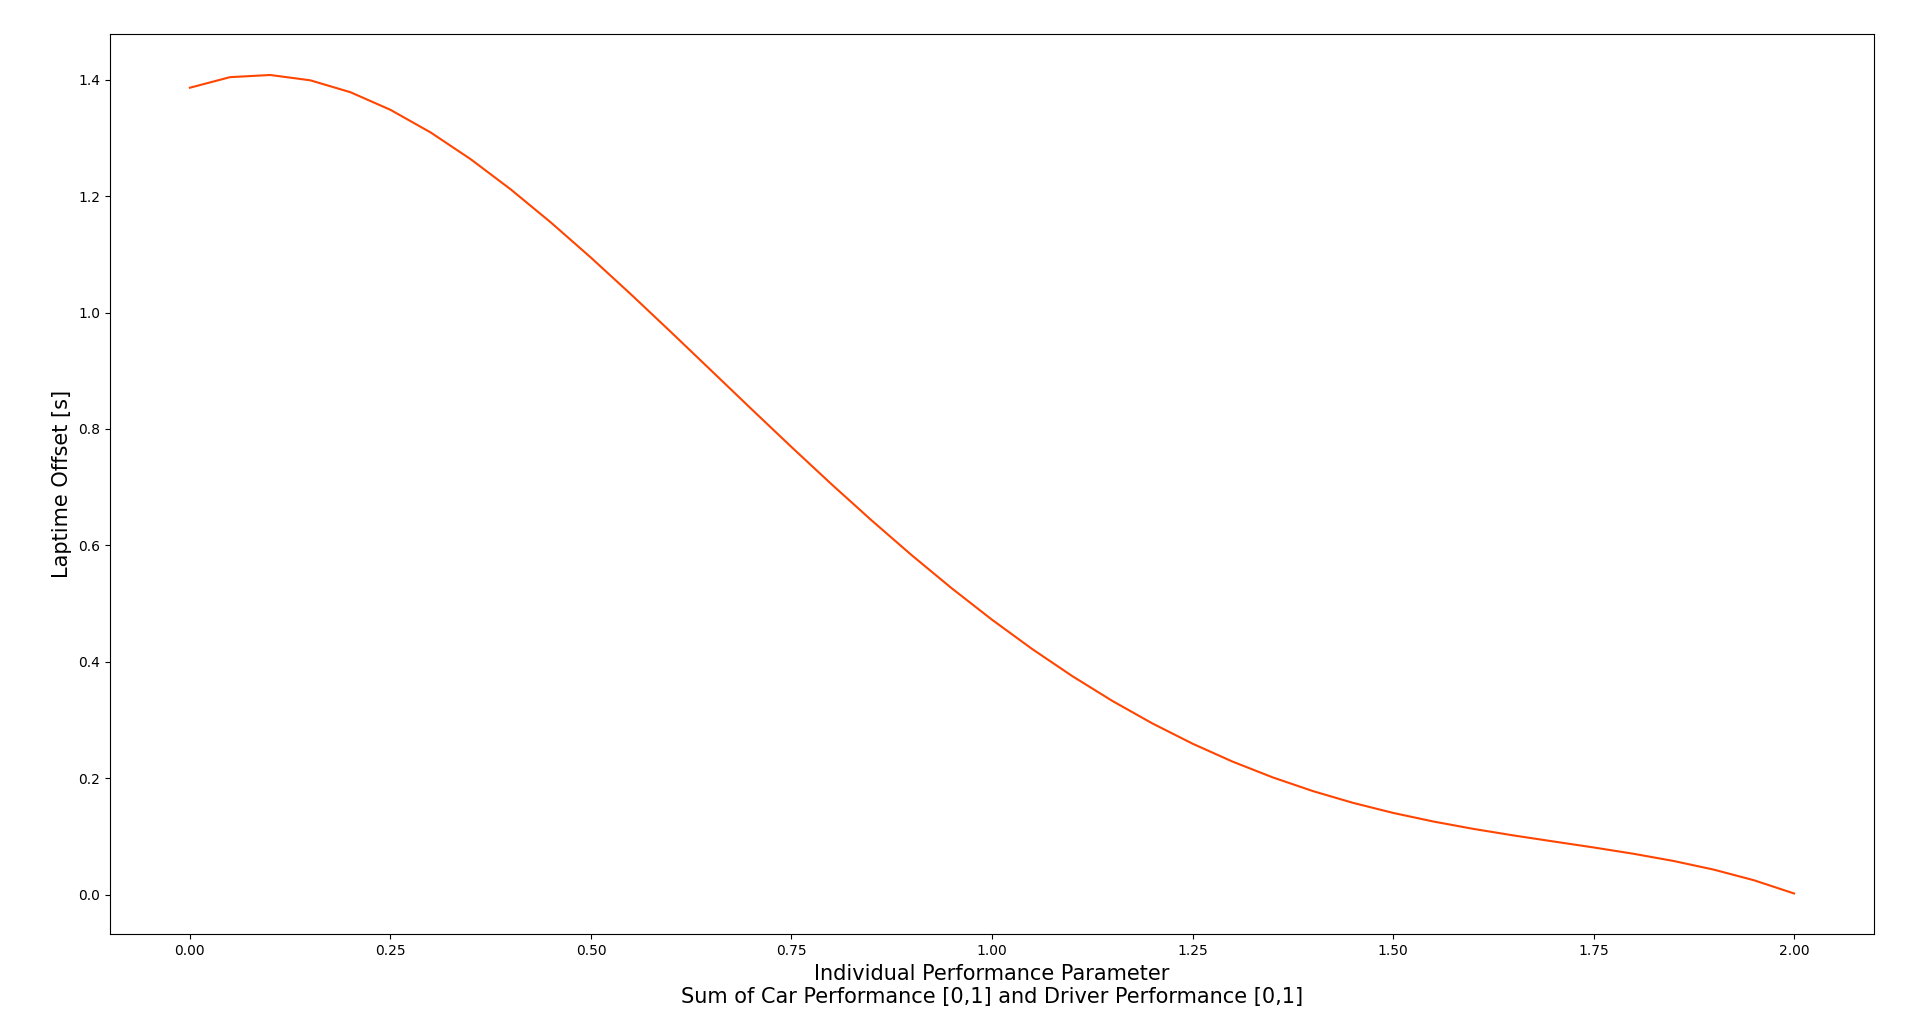
\includegraphics[scale=0.33]{Studienarbeit_F1/images/indivu_model_new_size.png}
    \caption{Individuelles Leistungsmodell}
    \label{fig:individual_model}
\end{figure}

Folgend dem Modell fährt ein Fahrzeug mit Leistungsparameter $0$ im Schnitt $1.4$ Sekunden langsamer pro Runde auf eine Rundenzeit von 80 Sekunden. Im mittleren Leistungsbereich, in welchem sich die meisten Fahrzeuge befinden, sind etwa eine zeitliche Differenz von $0.2$ - $0.5$ Sekunden pro Runde im Vergleich zum Optimum gegeben.

\subsubsection{Wechselwirkungsmodell}
% Fully corrected!
Das eingesetzte Wechselswirkungsmodell folgt dem Ziel, die in \ref{sec:race_behaviour} beschriebenen Einwirkungen von anderen Fahrzeugen auf ein einzelnes Fahrzeug abzubilden. Demnach muss das Modell den zusätzlichen Reifenverschleiß beim dichten Folgen eines anderen Fahrzeuges abbilden können, um somit den Verlust an aerodynamischen Abtrieb zu simulieren. \\
Zusätzlich muss entschieden werden, wie ein Überholmanöver stattfinden kann, sodass die Reihenfolge im Simulator konsistent bleibt. Zusätzlich soll ein Überholmanöver leichter gelingen, sollte der \gqq{Angreifer} ein schnelleres Tempo fahren können. Es muss also entschieden werden, ab wann die Möglichkeit zum Überholen besteht und unter welchen Umständen das Überholmanöver das Potential zu gelingen hat. Dies geschieht unter Berücksichtigung der Verteidigung durch das vorausfahrende Fahrzeug.\\
\\
Grundlegend wird davon ausgegangen, dass erst bei einem zeitlichen Delta von unter einer Sekunde zwischen zwei Fahrzeugen die Betrachtung des gegenseitigen Einflusses betrachtet werden muss. Innerhalb dieses Fensters ist ein Überholmanöver möglich, da das Auftreten des Windschattens eine erhöhte Spitzengeschwindigkeit auf den Geraden erlaubt. Dieser Windschatten verursacht aber wiederum in den Kurven, dass die Reifen mehr strapaziert werden müssen, um die Geschwindigkeit aufgrund des fehlenden Abtriebs zu halten. Entsprechend wurde diese Grenze als Schwellwert für die Betrachtung beider Wechselwirkungsmodelle genutzt.\\\\
Sollte nun ein Fahrzeug unter einer Sekunde hinter dem vorausfahrenden Fahrzeug sein, so wird das Alter des Reifens pro Runde zusätzlich um einen Faktor zwischen $[0.05, 0.25]$ erhöht. Dieses Intervall wurde abhängig vom Abstand zum vorausfahrenden Fahrzeug gemacht, um somit die verstärkende Wirkung bei abnehmenden Abstand zu repräsentieren. Das generierte Modell ist in Abbildung \ref{fig:add_tyre_degradation} zu sehen.\\
\begin{figure}
    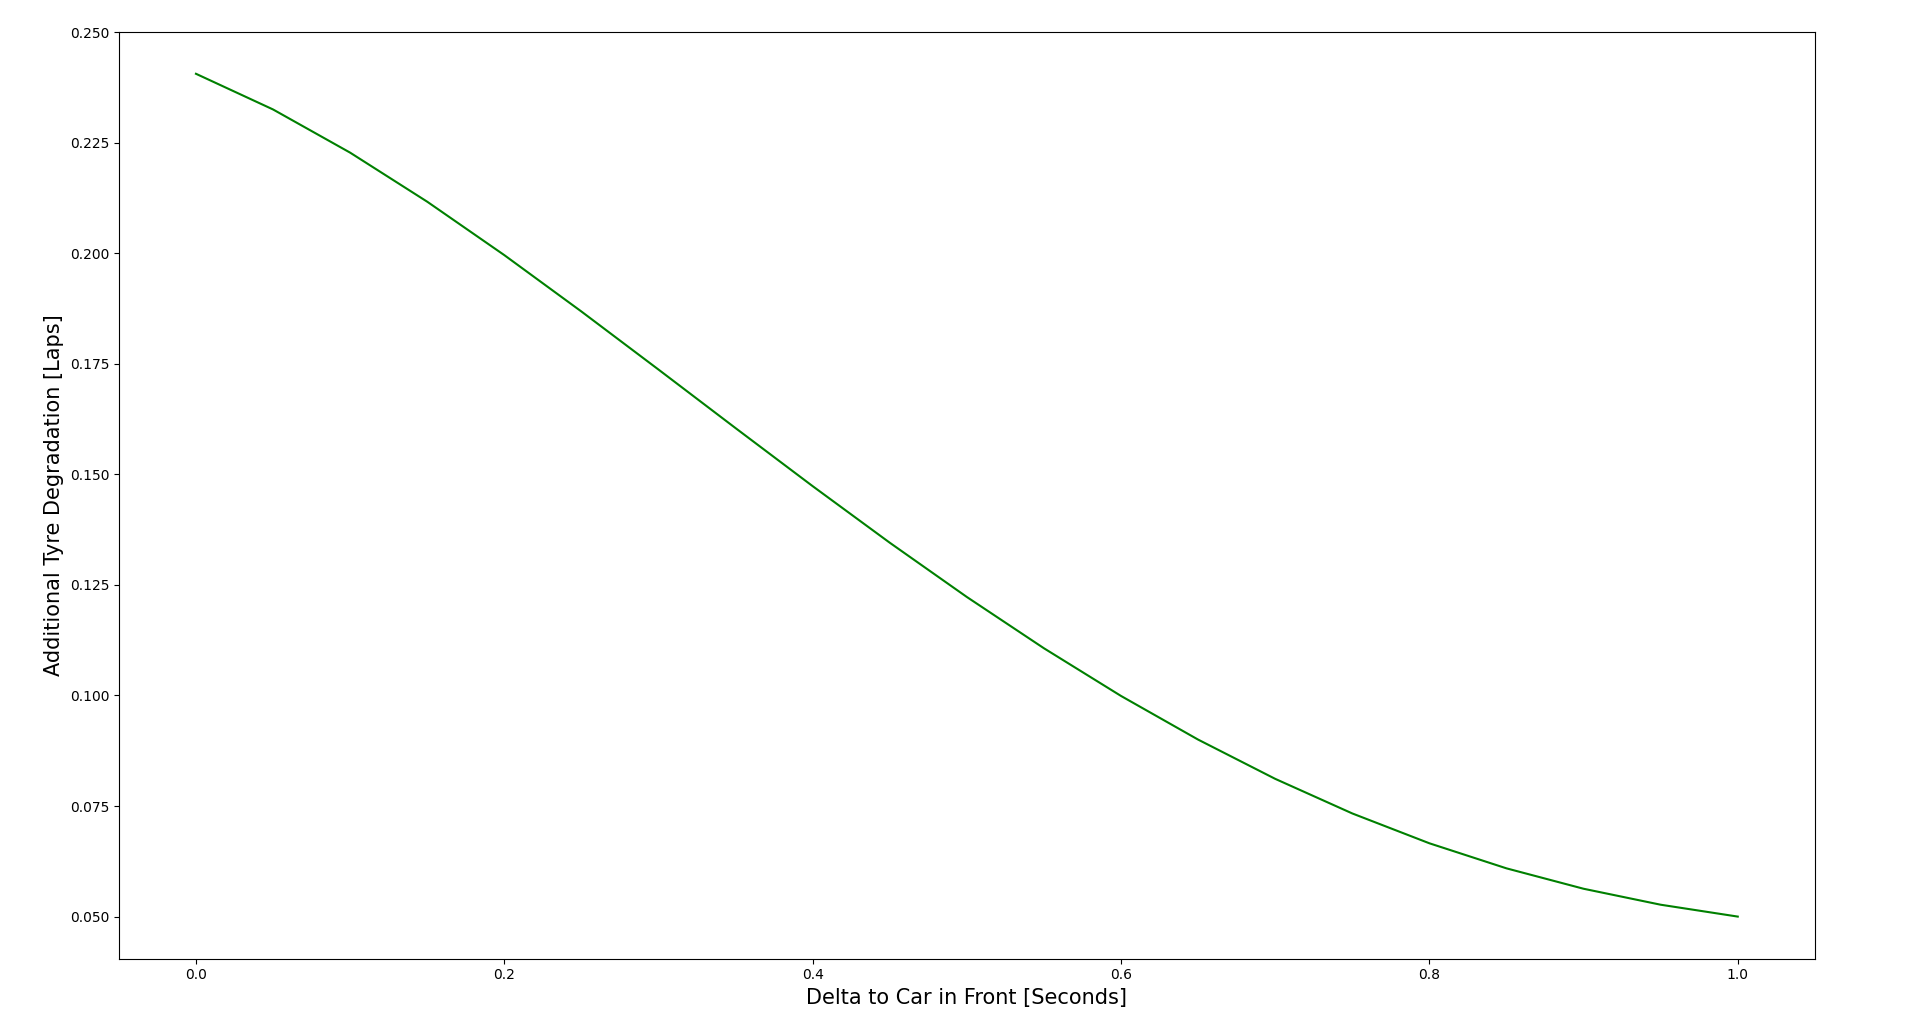
\includegraphics[scale=0.34]{Studienarbeit_F1/images/tyre_deg_new_size.png}
    \caption{Wechselwirkungsmodell für zusätzlichen Reifenverschleiß}
    \label{fig:add_tyre_degradation}
\end{figure}

\subsection{KI Modell}
% Tims Stuff :D
Als Basis für die finale KI zur Optimierung der Rennstrategie dienen die in Kapitel \ref{künstliche_Intelligenz} erarbeiteten Sachverhalte. Als RL-Algorithmus wurde sich aufgrund der Tests mit der einfachen KI für den \gqq{double-DQN} entschieden. Die zentrale Änderung des finalen Modells stellt die Größe des Zustands als Eingabe für das neuronale Netz dar. Dieser beinhaltet nun die gesamte verfügbare Information über denn Rennzustand. Eine Übersicht über die im Wesentlichen verfügbaren Informationen lässt sich in Abbildung \ref{fig:race_state} finden.
\begin{figure}
    \centering
    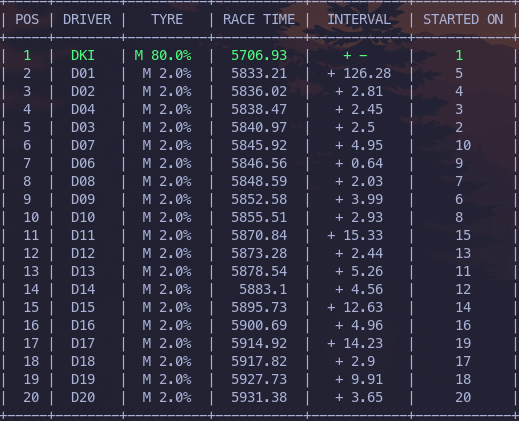
\includegraphics[scale=0.7]{Studienarbeit_F1/images/race_state.png}
    \caption{Verfügbare Informationen über jedes Auto am Ende eines Rennens}
    \label{fig:race_state}
\end{figure}
Zusätzlich wird für die Information über die bereits genutzten Reifentypen in Form eines Flags übergeben, um die Assoziation einer Disqualifikation mit der Nutzen von einer zu geringen Anzahl von verschiedenen Reifentypen zu ermöglichen. Eine vollständige Aufschlüsselung des Eingabezustands wie er im Code vorbereitet wird lässt sich in Listing \ref{lst:race_state} betrachten.

\begin{lstlisting}[label={lst:race_state}, caption={Ermittlung des Eingabezustands des neuronalen Netzes}, language={Python}]
def get_state(car: Car, lap : int):
    """
    return the current state for the AI - Input
    """
    # tyre degredation from 100% to 0%
    degredation = car.tyre.degredation * 100
    remaining_laps = RACE_DISTANCE - lap
    delta_to_leader = car.delta_to_leader
    # last lap time of the car
    lap_time = car.last_lap_time
    position = car.position
    # one hot coded : which compound is the car on?
    soft, medium, hard = one_hot_compound(car.tyre.compound)
    # have we used enough different compounds to not be disqualified?
    second_compound_flag = 1 if car.distinctUsedTyreTypes() >= 2 else 0
    delta_to_front = car.delta_to_car_infront if car.delta_to_car_infront != "-" else 0
    starting_pos = car.grid_position
    state_tensor = torch.tensor([degredation, remaining_laps, delta_to_leader, lap_time, position, soft, medium, hard, second_compound_flag, delta_to_front, starting_pos], dtype=torch.float32)

    return state_tensor
\end{lstlisting}
Basierend auf diesem Eingabezustand wurden die Hyperparameter des DQN manuell ermittelt. Einige der Parameter, die sich beim Ermittlungsprozess als besonders einflussreich herausgestellt haben, sind in Listing \ref{lst:hyperparams} dargestellt.
\begin{lstlisting}[label={lst:hyperparams}, caption={Ausgewählte, wichtige Hyperparameter des DQN}, language={Python}]
   layers = [11, 30, 30, 4]
   learning_rate = 1.5 * 1e-4
   episodes = 20000
   # keep 200 races in memory
   memory_size = 200 * race_length
   # amount of steps in the environment until memory is sampled
   sampling_period = 5
   # amount of transitions to sample from memory
   batchsize = 32
\end{lstlisting}

\subsection{KI Performance}\label{sec:ai_performance}
Abschließend gilt es die Leistung und das Verhalten eines trainierten Modells zu analysieren und zu vergleichen. Dabei können die von der KI erlernten Strategien untersucht und in Kontext der realen Verhältnisse gesetzt werden. Hierzu werden verschiedene Szenarien mit einem vortrainierten Modell untersucht, dabei soll insbesondere das Verhalten der KI in extremen Szenarien, welche als Grenzfälle betrachtet werden können, analysiert werden. Die Szenarien unterscheiden sich dabei einerseits in die Startposition des KI-Fahrzeuges sowie in der Leistung des Autos. Das untersuchte Modell sollte im Training jede Start-Position bereits erfahren haben und sollte sich dabei in verschieden starken Fahrzeugen befanden haben.\\\\
Bei der Betrachtung der Performance gilt es die Stabilität der Resultate der KI über eine Vielzahl von Rennen zu betrachten, um so zum einen eine Aussage über die Realitätsnähe des Simulators sowie die Leistungsfähigkeit und Qualität der KI machen zu können.\\
Das restliche Feld, mit welchem die KI konkurriert, fährt dabei eine statische Strategie. Diese Strategie ist durch vorangegangene Test gewählt, da diese statische Strategie oft von der KI gewählt und genutzt wurde. Somit startet das Feld auf Softs und fährt in den Runden 15 und 45 an die Box und wechselt dabei auf Mediums. 

\subsubsection{Szenario 1: Leistungsstärkstes Auto auf Pole-Position}\label{sec:best_car_pole}
Das nachfolgend betrachtete Szenario entspricht vor dem Hintergrund seiner Situationsparameter der optimalen Ausgangslage eines Teilnehmenden in der Formel 1.\\
Der Teilnehmende startet von der vordersten Start-Position und hat aus diesem Grund eine vorteilhafte Position innerhalb des Rennens inne. Außerdem hat das untersuchte Fahrzeug die stärksten Leistungsparameter mit den Werten für Fahrerleistung und für Fahrzeugleistung jeweils gleich eins.\\
Dieses Szenario erlaubt die Untersuchung, ob die KI tatsächlich eine optimale Strategie wählt und entsprechend die Start-Position beziehungsweise die Führung halten kann oder sogar den Abstand zum ersten Verfolger ausbauen kann. Diese Erwartung gegenüber des Szenarios wird durch den Umstand des performantesten Fahrzeuges zusätzlich verstärkt. Es ist somit zu erwarten, dass bei der Betrachtung einer Vielzahl von Renndurchläufen insgesamt die Anzahl der erreichten ersten Plätze in der Gesamtheit aller Rennsimulationen massiv überwiegen sollte.
\\
\begin{figure}
    \centering
    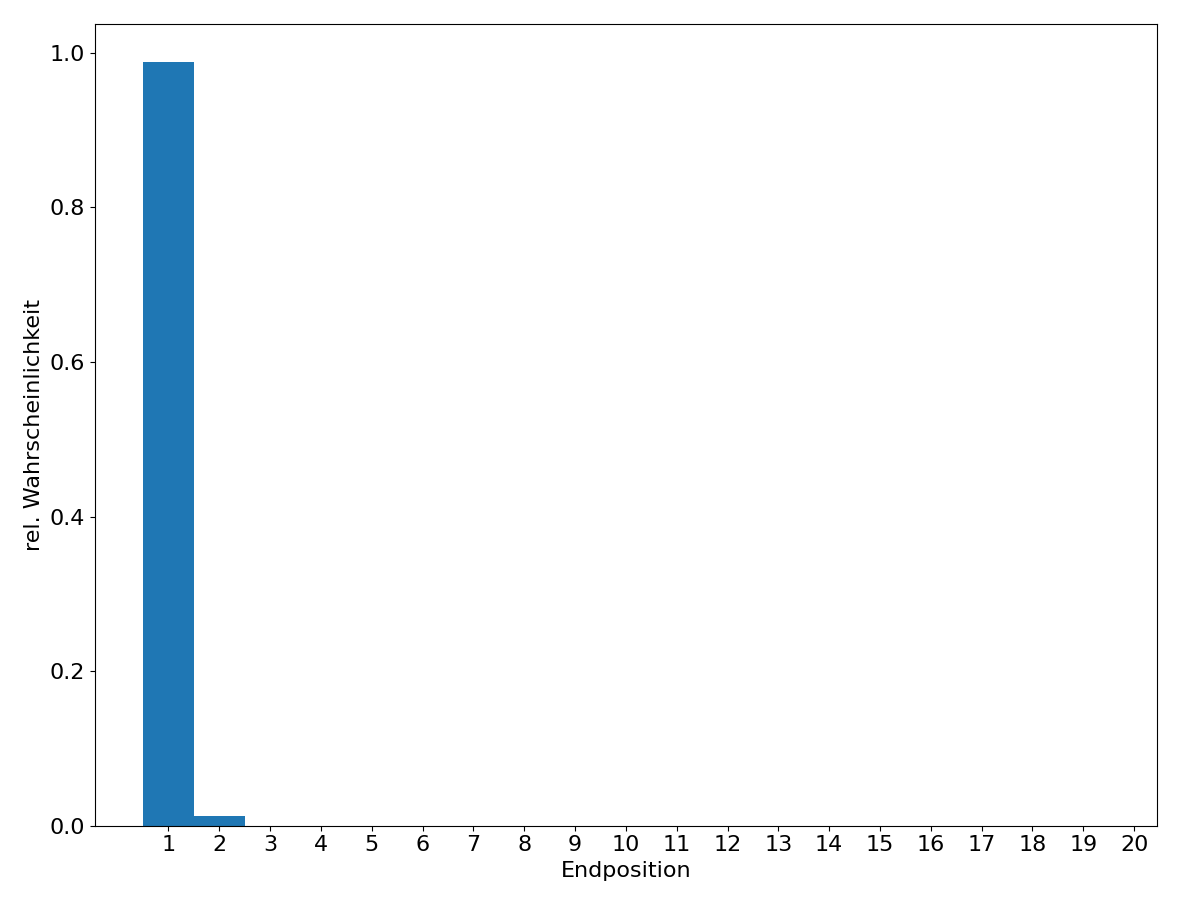
\includegraphics[scale=0.5]{Studienarbeit_F1/images/hist_best_car_pole.png}
    \caption{Szenario 1: Anteile der Platzierungen bei 1000 Renndurchläufen}
    \label{fig:hist_best_car_pole}
\end{figure}
\\
Zur Untersuchung der Stabilität und längerfristigen Performance der KI wurden die Rennergebnisse über 1000 Renndurchläufe bei den zuvor genannten Parametern betrachtet und ausgewertet. Die dabei erreichten Rennplatzierungen sind in Abbildung \ref{fig:hist_best_car_pole} in Form eines Histogramms dargestellt.\\
Hierbei zeigt sich bis auf einen sehr kleinen Anteil an zweiten Plätzen eine Bestätigung des erwarteten Verhaltens in Form eines großen relativen Anteils von Rennsiegen.\\
Dieses stabile Verhalten unterstreicht die Performance der KI. Es gelingt in der absoluten Mehrzahl der Fälle, die Führungsposition gegen die Konkurrierenden im Feld zu verteidigen. Der seltene Fall des zweiten Platzes kann als Bestätigung der Performance interpretiert werden, da maximal eine einzige Platzierung gegenüber den Konkurrierenden eingebüßt wird.
\\
\begin{figure}
    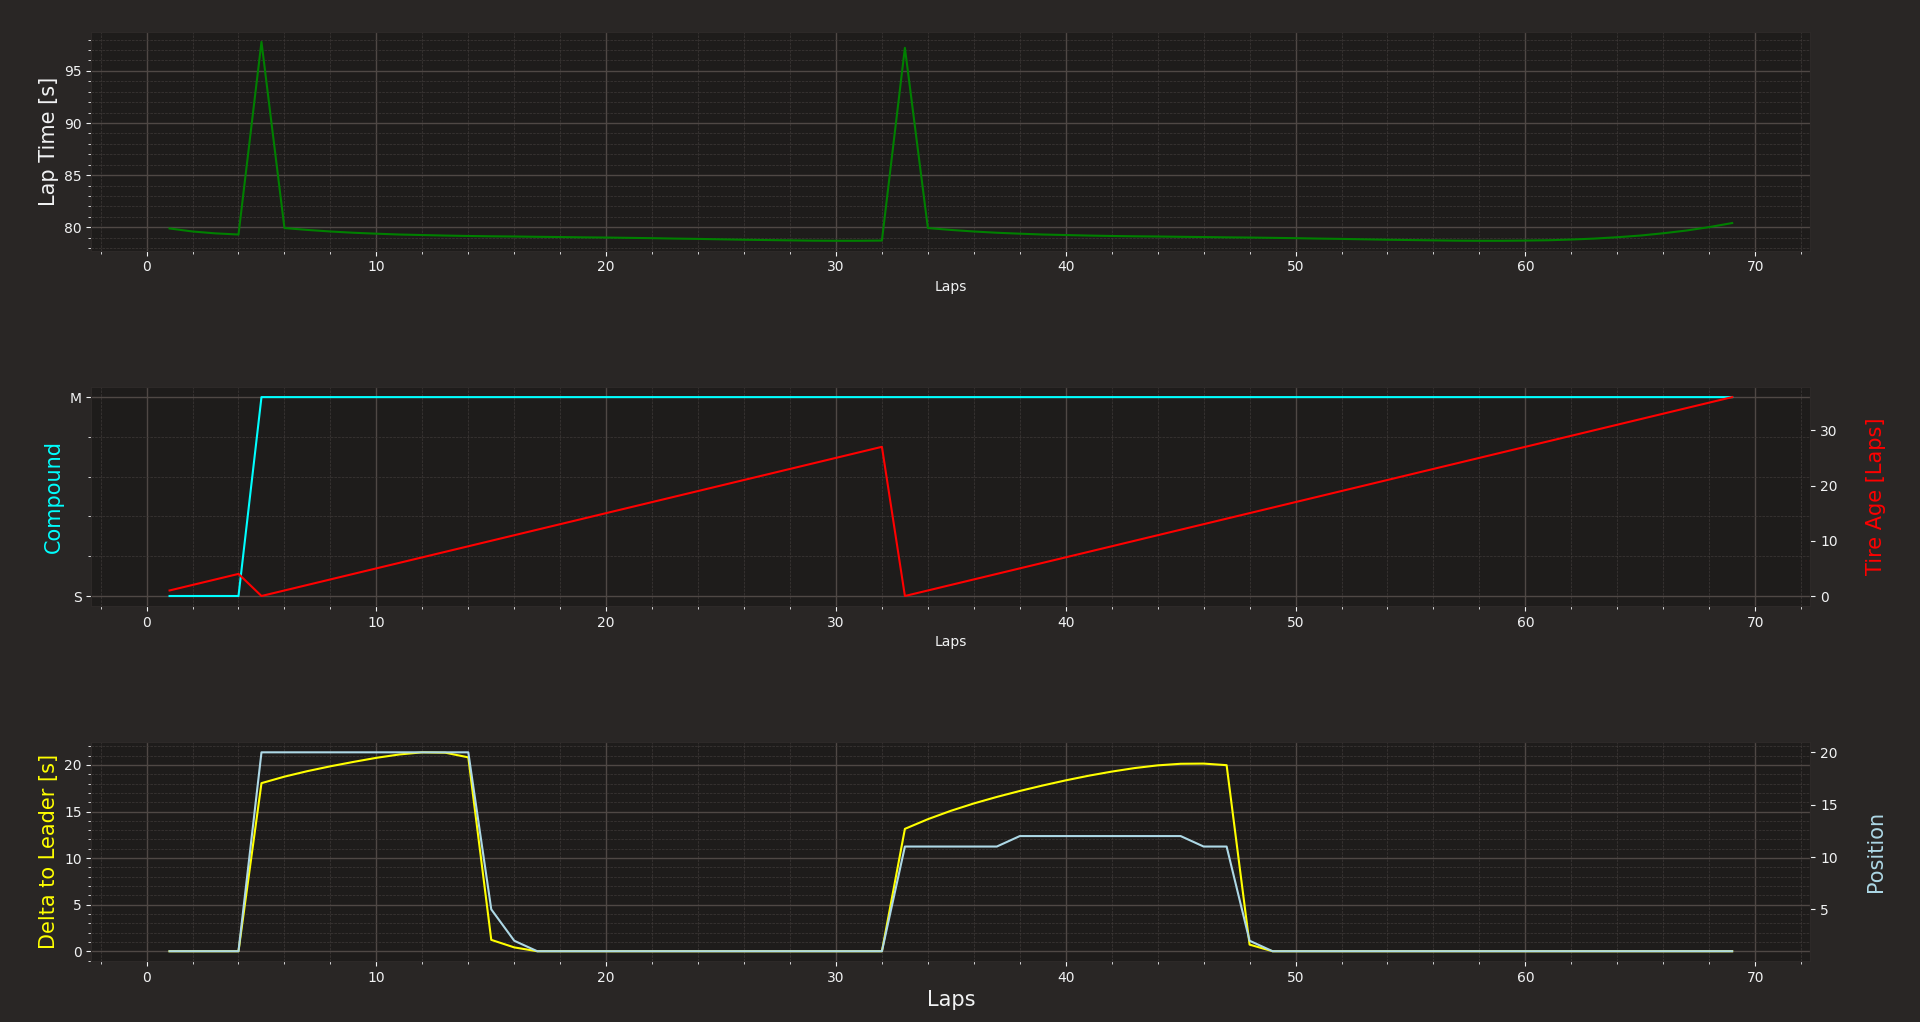
\includegraphics[scale=0.325]{Studienarbeit_F1/images/eval_best_pole_stayed_first.png}
    \caption{Beispielhaftes Verhalten Szenario 1 - Start von Pole - Platz 1 im Ziel}
    \label{fig:example_scenario_one}
\end{figure}
\\
Zur Veranschaulichung des Verhaltens der KI über ein einzelnes Rennen hinweg sind in Abbildung \ref{fig:example_scenario_one} die Abläufe eines einzelnen Rennens dargestellt. Im obersten Graph findet sich die Rundenzeit der KI wieder, Hier sind die zwei gewählten Boxenstopps der KI deutlich als Ausreißer nach oben zu erkennen. Hierbei startet die KI auf Soft und wechselt anschließend zwei Mal auf Mediums.\\
Entsprechend verliert die KI die Führung, welche sie aber mit dem Boxenstopp des restlichen Feldes wiedererlangen kann.\\
Aus analytischer Sicht zeigt der Rennsimulator sehr aussagekräftige und realistische Verhältnisse in diesem Szenario. So ist Überholen möglich und machbar, aber auch nicht zu einfach. Aus strategischer Sicht ist hierbei interessant, dass die KI beide Boxenstopps früher ansetzt als das restliche Feld und dadurch sogar kurzzeitig den letzten Platz belegt. Dieser frühere Boxenstopp aber offensichtlich der gesamten Rennzeit nicht schadet und die KI somit den Sieg halten kann trotz des zunehmenden Verschleißes am Ende des Rennens.

\subsubsection{Szenario 2: Leistungsschwächstes Auto auf Pole-Position}
% Car Parameters = 0.4
Das folgende Szenario soll ein Rennen von der Pole-Position aber dafür im Auto mit den schlechtesten Individual-Leistungswerten abbilden. Dies dient rein zur wissenschaftlichen Untersuchung des Verhaltens der KI und des Simulators, da das Szenario in der realen Formel 1 sehr unrealistisch ist. Entsprechend erlaubt diese Analyse besonders Rückschlüsse auf die Korrektheit der eingesetzten Modelle im Simulator.\\
Es wird also erwartet, dass das Fahrzeug auch bei durch die KI optimierter Strategie im Fahrerfeld stark zurückfallen wird und somit das Rennen außerhalb der Top 10 beenden sollte.\\
\begin{figure}
    \centering
    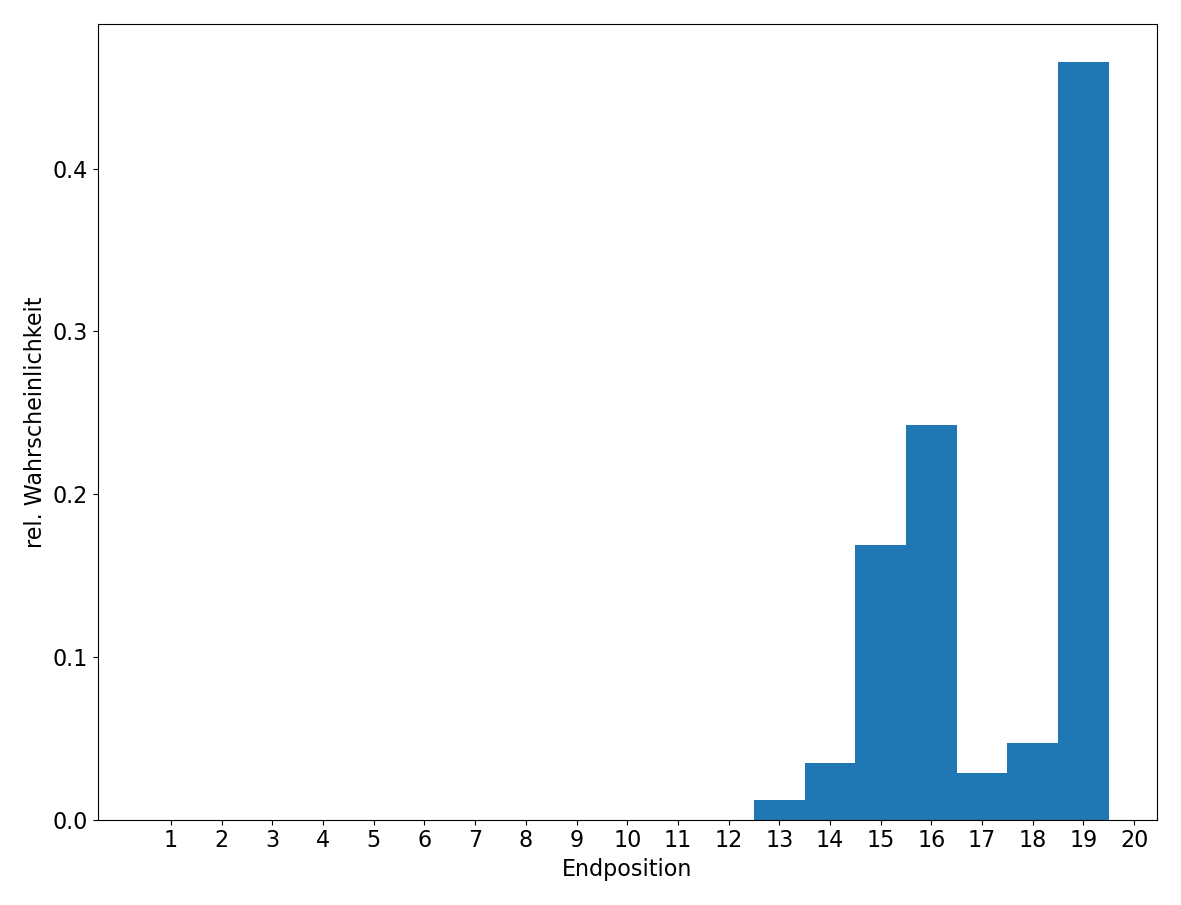
\includegraphics[scale=0.5]{Studienarbeit_F1/images/hist_worst_car_pole.png}
    \caption{Szenario 2: Anteile der Platzierungen bei 1000 Renndurchläufen}
    \label{fig:hist_worst_car_pole}
\end{figure}
Eine Betrachtung der Resultate über 1000 Rennen liefert auch in diesem Szenario eine Bestätigung der zuvor aufgestellten These hinsichtlich der erwarteten Leistungen der KI innerhalb des Rennens. In der Abbildung \ref{fig:hist_worst_car_pole} ist zu erkennen, dass trotz der zunächst optimalen Ausgangslage am Beginn des Rennens kein Ergebnis unter den Top 10 erzielt werden konnte, sondern sich die Resultate im letzten Drittel des Feldes konzentrieren. Diese Auswertung bestätigt den signifikanten Einfluss der Leistungsparameter auf die schlussendlichen Rennresultate. Es wird der Realität entsprechend aufgezeigt, dass trotz einer potenziell optimalen Rennstrategie in einem nicht konkurrenzfähigen Auto keine guten Platzierungen erreicht werden können.\\
\begin{figure}
    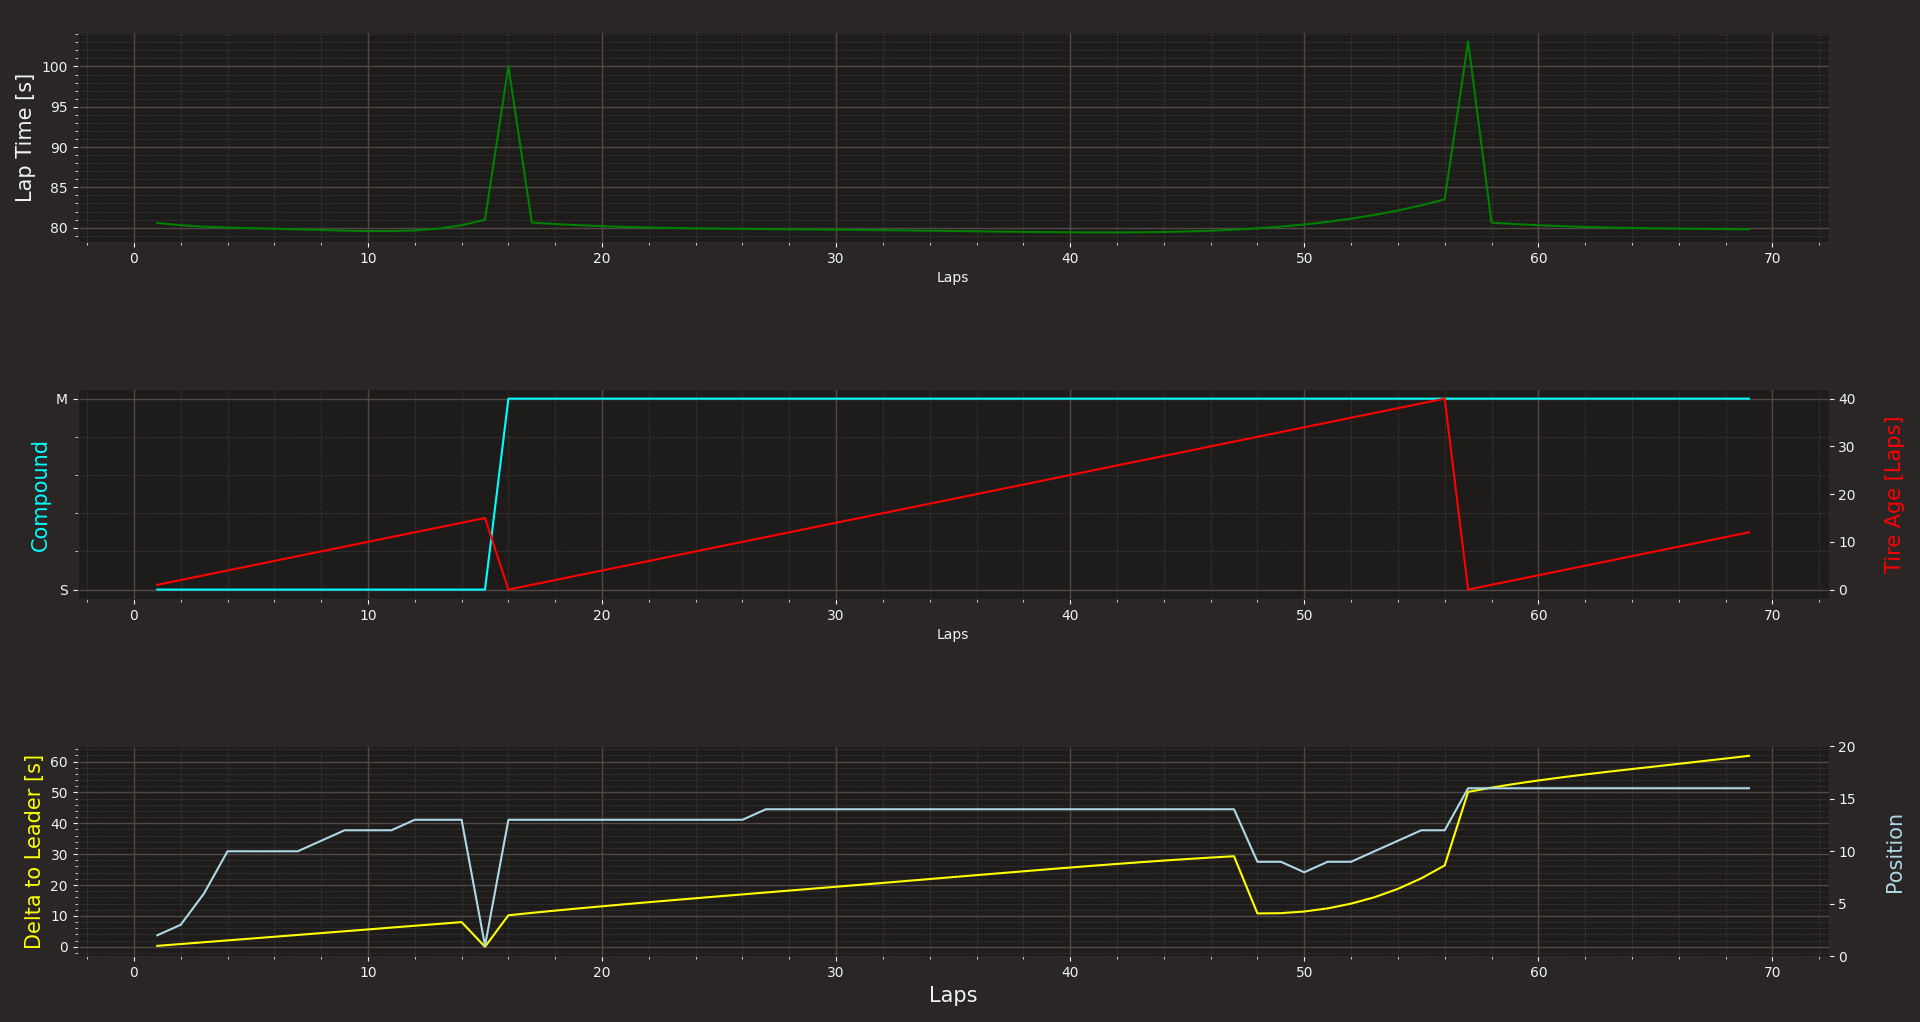
\includegraphics[scale=0.325]{Studienarbeit_F1/images/eval_worst_pole_new_got_16.png}
    \caption{Beispielhaftes Verhalten Szenario 2 - Start von Pole - Platz 15 im Ziel}
    \label{fig:example_scenario_two}
\end{figure}
Ebenfalls wird in diesem Szenario ein einzelnes Rennen beispielhaft in Abbildung \ref{fig:example_scenario_two} betrachtet. In diesem Fall ist besonders schön der Einfluss der Leistungsparameter auf die Rundenzeit durch die Individual-Modelle zu sehen. So verliert unsere KI kontinuierlich pro Runde an Zeit auf den Führenden (zu sehen im gelben Graph) trotz einer ähnlichen Strategie. Die Individual-Modelle funktionieren ebenso wie erwartet und erlauben eine reelle Abbildung der Leistung auf die Rennzeit als Ganzes. Dadurch kann unsere KI im schlechtesten Wagen die Führung nicht halten und landet auf Platz 15. Hierbei ist ebenfalls schön zu beobachten, dass die vorderen Positionen sehr schnell innerhalb von 15 Runden verloren werden, danach aber der Verlust langwierig ist. Dies resultiert aus den Leistungsunterschieden innerhalb des Fahrer-Feldes. Dabei befindet sich die KI zunächst in direktem Positionskampf mit den leistungsstärksten Konkurrierenden, welche entsprechend einfach die KI überholen können. Im späteren Rennverlauf befindet sich die KI im Umfeld schwächerer Gegner, welche nicht mehr in diesem Maße leistungsstärker sind und es folglich schwerer haben, dass leistungsschwächste Fahrzeug zu überholen. Dies bedeutet Überholen ist möglich, aber erst bei entsprechendem Tempo einfach. Ansonsten bleibt es eine Herausforderung, so wie es die reellen Verhältnisse vorgeben.


\subsubsection{Szenario 3: Leistungsstärkstes Auto ab letzter Start-Position}

Um eine tiefgreifendere Aussage über die Wechselwirkungsmodelle treffen zu können, muss entsprechend untersucht werden, ob das Überholen mit dem notwendigem Tempo zu leicht beziehungsweise zu schwer ist. Entsprechend wird hierbei ein Szenario gewählt, welches stark das Überholen fördert und provoziert, in dem die KI im performantesten Fahrzeug von der letzten Start-Position starten muss.\\
Hierbei wird kein Rennsieg erwartet, da dies in Anbetracht des restlichen Fahrerfeldes unrealistisch ist. Dennoch sollte ein klarer Fortschritt durch das Feld ersichtlich sein und die KI somit die Top 10 erreichen.
\\
\begin{figure}
    \centering
    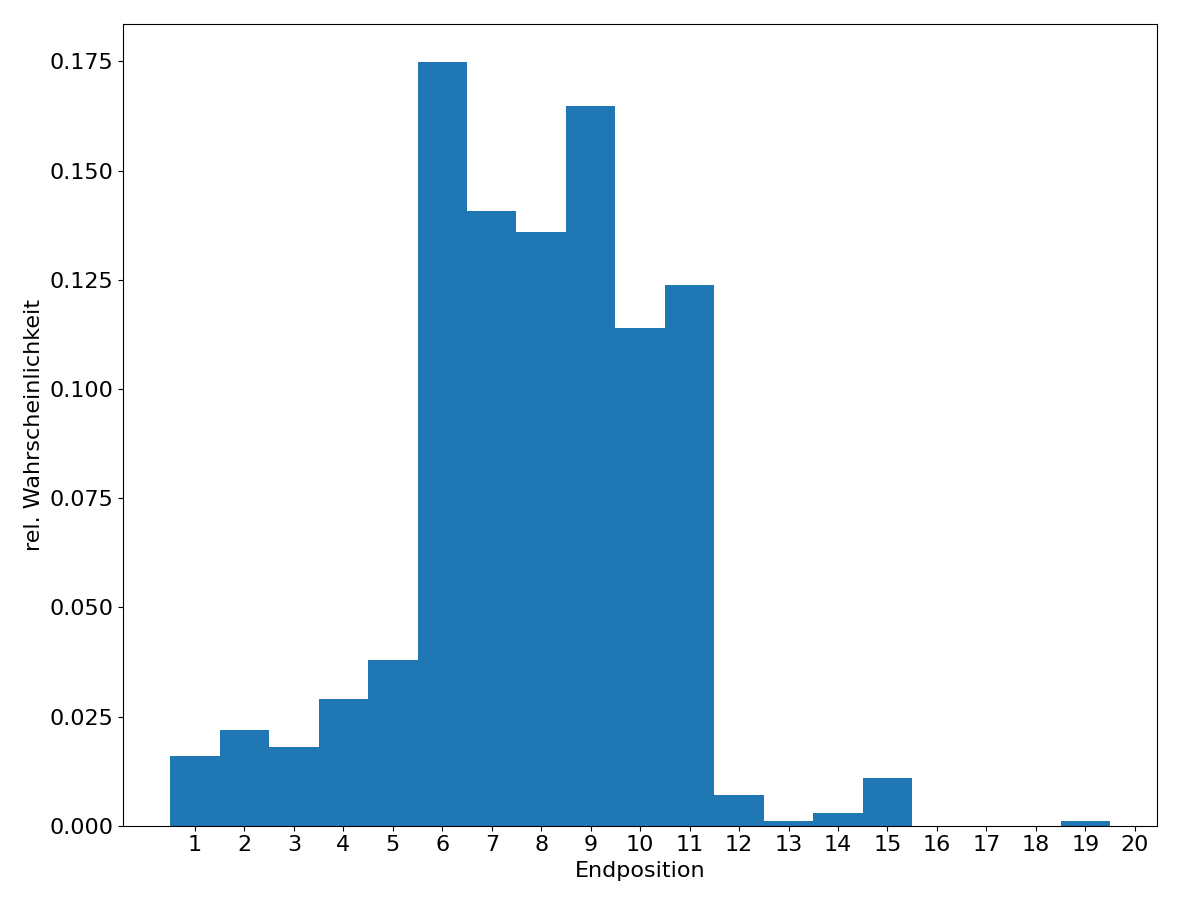
\includegraphics[scale=0.5]{Studienarbeit_F1/images/hist_best_car_from_back.png}
    \caption{Szenario 3: Anteile der Platzierungen bei 1000 Renndurchläufen}
    \label{fig:hist_best_car_from_back}
\end{figure}
\\
Im Zuge der längerfristigen Betrachtung der Resultate in Abbildung \ref{fig:hist_best_car_from_back} bestätigt sich die zuvor aufgestellte Vermutung an die Performance der KI. Es ist zu erkennen, dass die KI klare Erfolge innerhalb des Feldes erzielt und Plätze gut machen kann. Dies zeigt sich an dem sehr geringen Anteil an hinteren Positionen [12;20], die während der 1000 Renndurchläufe erzielt wurden.\\
Zeitgleich ist der Anteil an Podiumspositionen ebenfalls relativ gering, da in diesem Konkurrenzfeld gegen stärkere Gegner angetreten werden muss und ein Überholen mit weiterem Vorankommen deutlich erschwert wird.\\
Mit bei weitem größten Anteil hat die KI auf Basis dieser Leistungsparameter einen Rennabschluss in der Mitte des Feldes [6;11] erreicht. Damit kann die KI-Strategie in diesem Anwendungsszenario als stabil betrachtet werden.
\\
\begin{figure}
    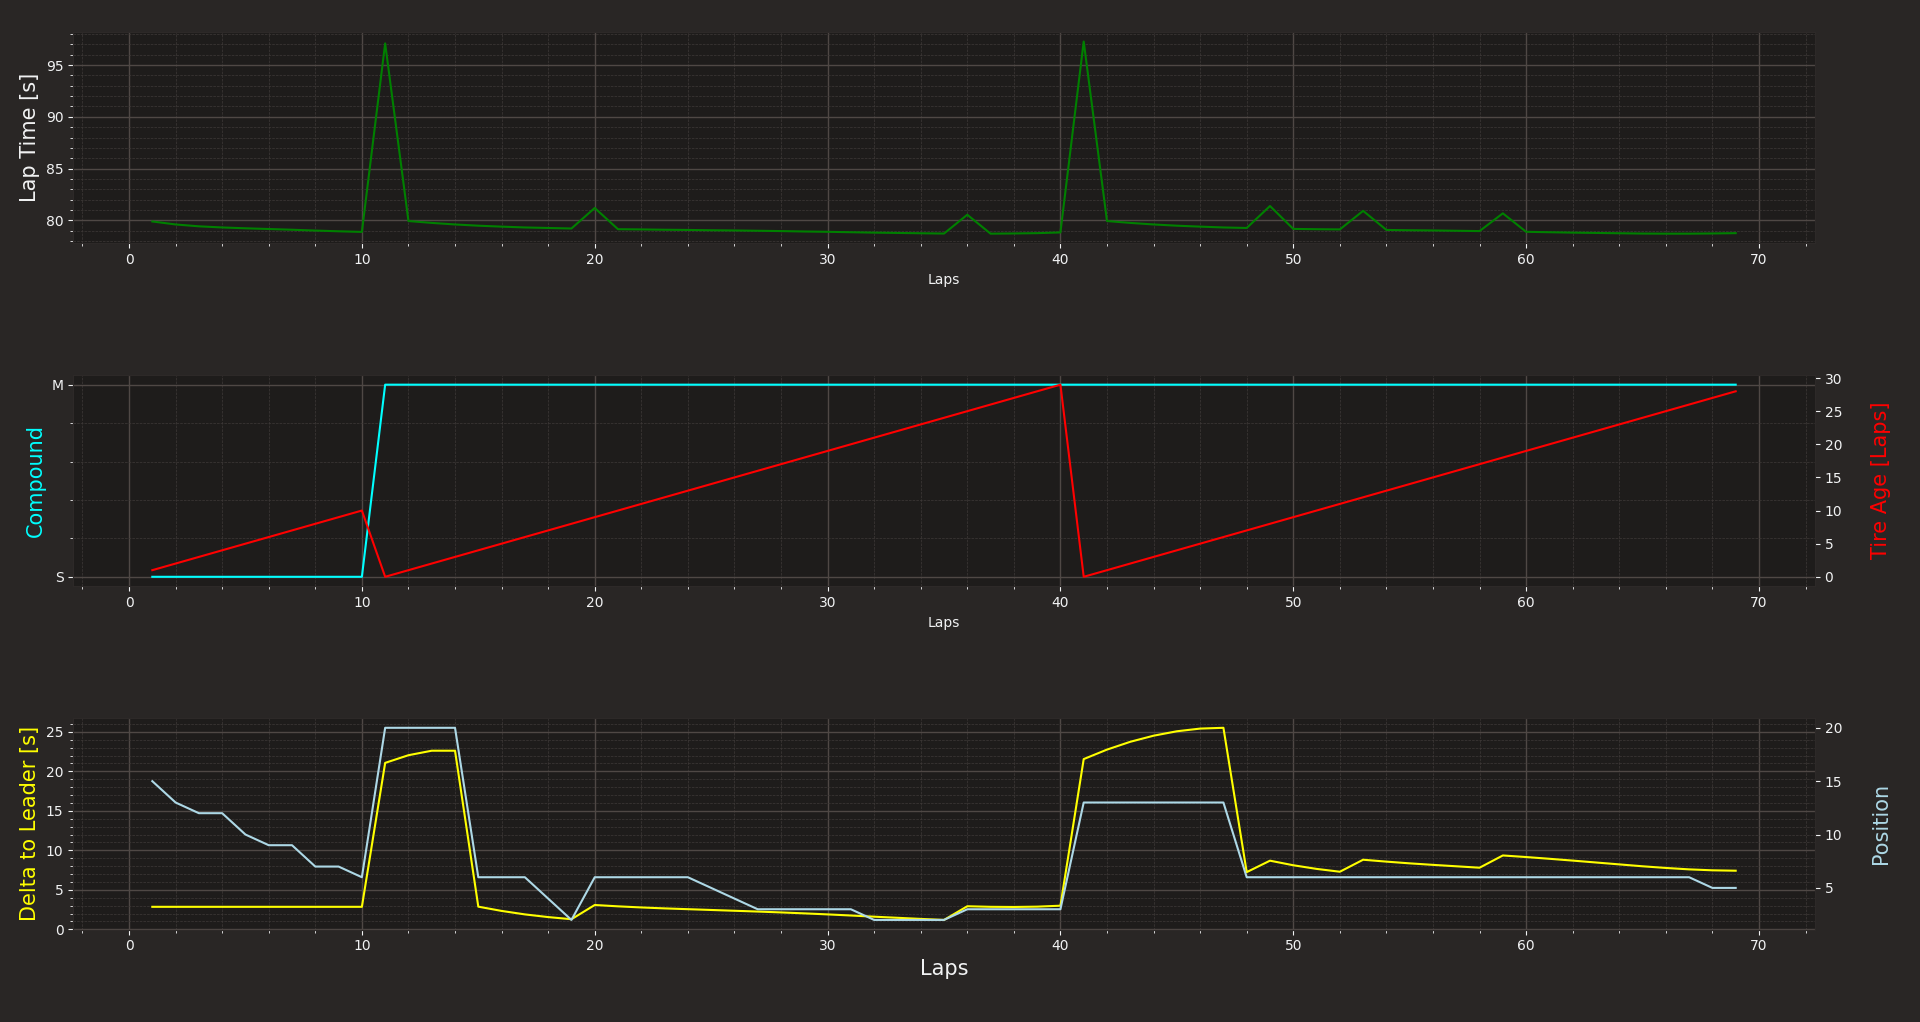
\includegraphics[scale=0.325]{Studienarbeit_F1/images/eval_best_from_last_new_got_5.png}
    \caption{Beispielhaftes Verhalten Szenario 3 - Start vom letzten Platz - Platz 5 im Ziel}
    \label{fig:example_scenario_three}
\end{figure}
\\
In der beispielhaften Untersuchung eines einzelnen Rennens in Abbildung \ref{fig:example_scenario_three} bestätigt sich die optimale Strategie mit einem initialem Stint auf Soft und zwei Stints auf Mediums, welche die KI wählt.\\
Aus Simulator Sicht sind an dieser Stelle die Ausreißer in der Rundenzeit interessant, welche neben den normalen Boxenstopps zu sehen sind. Diese zeigen deutlich, dass das Fahrzeug in diesen Runden an einem Überholmanöver scheiterte und so durch das restliche Fahrerfeld aufgehalten wurde. Dies bestätigt wiederum die Funktionsweise und Wirkung der Wechselwirkungsmodelle des Simulators.


\subsubsection{Szenario 4: Leistungsschwächstes Auto ab letzter Start-Position}

Um zusätzlich das Verhalten der KI vollständig zu verifizieren, wird in diesem Szenario der umgekehrte Fall zum Verhalten in \ref{sec:best_car_pole} untersucht. Entsprechend wird die schlechteste Ausgangslage für ein Formel 1 Fahrzeug angenommen mit schlechtestem Auto und der hintersten Start-Position. Hierbei liegt die Erwartung, dass die KI es potentiell schafft, einzelne Plätze gut zu machen durch die optimierte Strategie. Ein Erreichen der Top 10 ist aber allein durch die Modelle des Simulators höchst unwahrscheinlich.
\\
\begin{figure}[H]
    \centering
    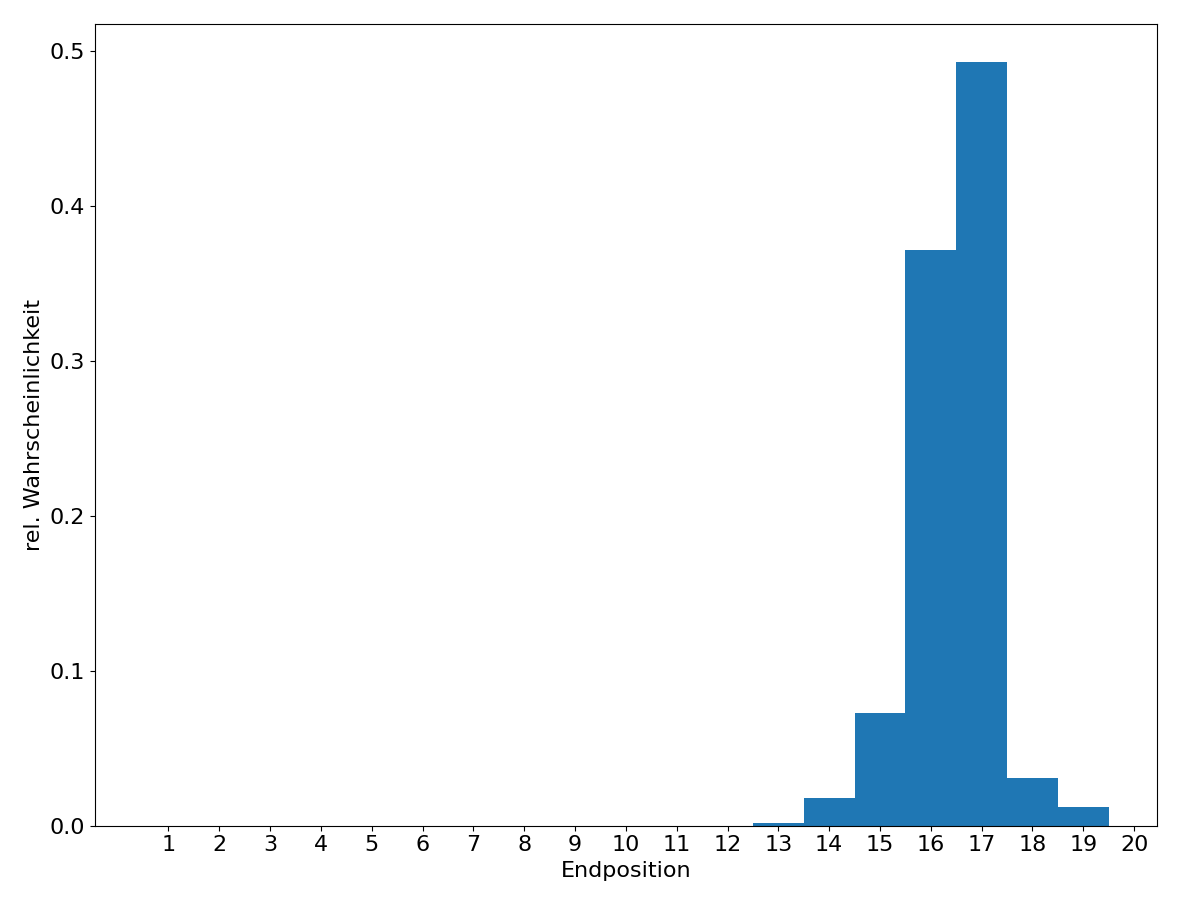
\includegraphics[scale=0.5]{Studienarbeit_F1/images/hist_worst_car_from_back.png}
    \caption{Szenario 4: Anteile der Platzierungen bei 1000 Renndurchläufen}
    \label{fig:hist_worst_car_from_back}
\end{figure}
Auch in diesem Szenario bestätigt sich das prognostizierte Verhalten, wie dem Histogramm \ref{fig:hist_worst_car_from_back} zu entnehmen ist. Aufgrund des leistungsstärkeren Konkurrenzfeldes ist es der KI nicht möglich, vordere Platzierungen zu erreichen, sondern befindet sich im Positionskampf mit schwächeren Gegnern im hinteren Teil des Feldes. Hier zeigt das Histogramm, dass es gelingt, einzelne Platzierungen gut zu machen und im Mittel Platzierungen um den 16 und 17 Rang zu erreichen. Dieses Ergebnis bestätigt den Vorteil der KI hinsichtlich der Rennstrategie, da es ihr gelingt, trotz eines leistungsschwachen Autos vereinzelte Plätze gutzumachen.
\\
\begin{figure}[H]
    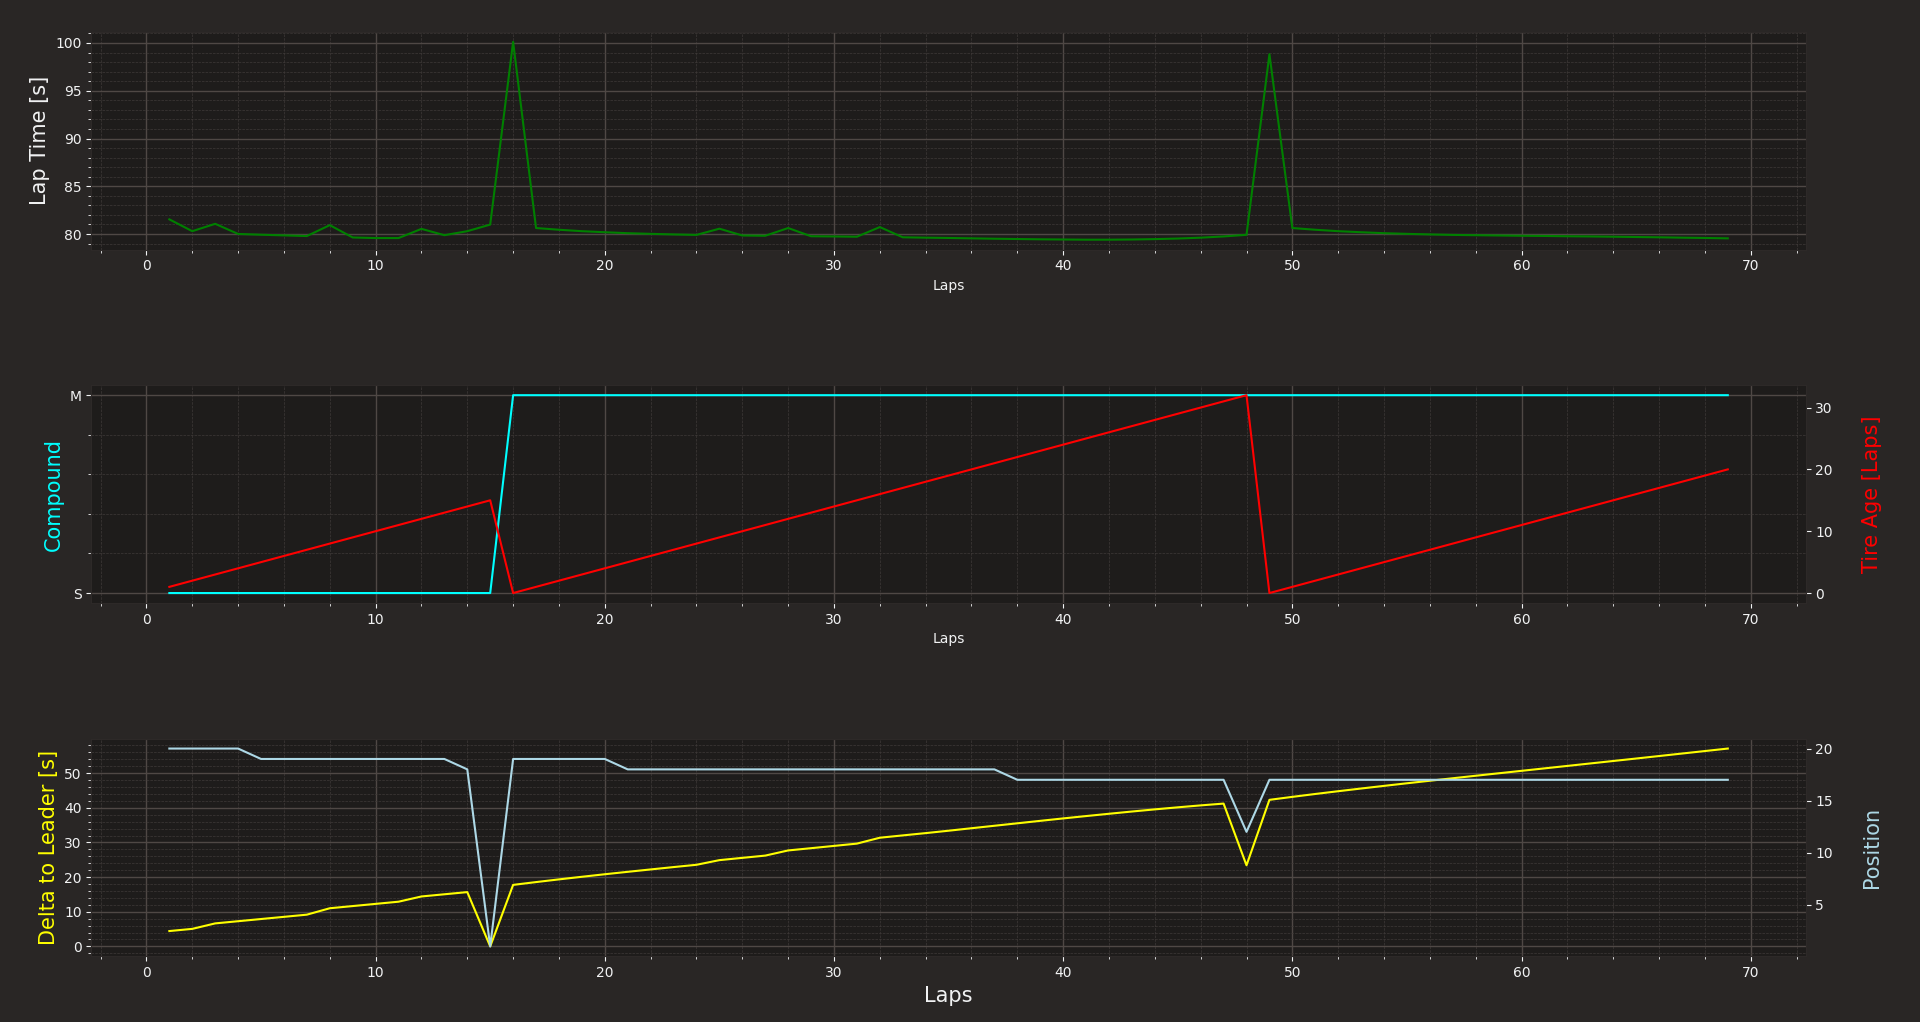
\includegraphics[scale=0.325]{Studienarbeit_F1/images/eval_worst_last_got_17.png}
    \caption{Beispielhaftes Verhalten Szenario 4 - Start vom letzten Platz - Platz 17 im Ziel}
    \label{fig:example_scenario_four}
\end{figure}
Auch in diesem Beispiel (siehe Abbildung \ref{fig:example_scenario_four}) sind die Einflüsse der anderen Fahrer im Feld deutlich in den Rundenzeit zu sehen. Dennoch schafft die KI mit besserer Strategie auch mit dem schlechtesten Fahrzeug einzelne Positionen gut zu machen und schafft somit den Sprung von Platz 20 auf Platz 17 im Ziel.\\\\
Im Allgemeinen ist über alle Szenarien hinweg auffallend, dass die KI identische Strategien wählt. Dieser Umstand wird im folgenden Kapitel \ref{sec:discussion} näher erläutert.




	\section{Diskussion}\label{sec:discussion}
% Keine wirkliche Auswertung der Daten für die Wechselwirkungsmodelle
% Überholen potentiell zu einfach und nicht repräsentativ sieht aber in den Auswertungen bisher sehr gut aus
% Eintönige Strategie Wahl! -> zu einfaches Modell führt zu einfachem optimierten Fall -> keine Varianz
Durch die Auswertung des Verhaltens der KI in den verschiedenen Szenarien in \ref{sec:ai_performance} konnten Rückschlüsse auf die Gültigkeit der eingesetzten Modelle im Simulator geschlossen werden. So konnten besonders der Reifenverschleiß, die Leistungsparemeter eines einzelnen Fahrzeuges und die Wechselwirkungen der Fahrzeuge untereinander verifiziert und beobachtet werden.\\
Einschränkend ist hierbei aber zu erwähnen, dass bei der Untersuchung der Reifen die Mischungen nicht bis auf die offiziellen Kategorien C1-C5 aufgelöst wurden. Dies ist durch den Umstand der Datenlage gegeben, welche ebenfalls eine Vereinfachung auf Soft, Medium und Hard vornimmt. Der Einfluss dieser Abstraktion wird als sehr gering eingestuft, muss aber für eine potentielle Weiterführung oder einen Live-Einsatz beachtet werden.\\
Weiter ist zu erwähnen, dass die Generierung der Wechselwirkungsmodelle vereinfacht aus der Datengrundlage abgeleitet wurden. Dies ist durch den Umstand gegeben, dass beispielsweise der zusätzliche Reifenverschleiß nicht aus den Daten ersichtlich ist und somit nur im Rahmen der bekannten Rennen geschätzt werden konnte. Entsprechend verhält es sich mit der kalkulierten Wahrscheinlichkeit für das Gelingen eines Überholmanövers, welches so gewählt werden musste, dass das Überholen nicht zu leicht fällt, aber auch nicht unmöglich ist.
\\\\
%KI Dinge, der dem was einfällt kann hierzu gerne noch was schreiben
Im Kontext der KI - Entwicklung lässt sich festhalten, dass an verschiedenen Stellen Designentscheidungen getroffen wurden, die lediglich auf Heuristiken und keinerlei objektiven Metriken basieren. Dies gilt sowohl für die Hyperparameter und hidden-layer Größen des neuronalen Netzes als auch für elementare Bestandteile des finalen DQN-Lernprozesses wie der Belohnungsfunktion. Somit sind die im Rahmen der Arbeit erzielten Ergebnisse mit großer Sicherheit mit mehr Zeitaufwand noch zu verbessern. Ebenso ist es durch die instabile Natur der Derivate des DQN-Algorithmus nicht möglich, eine verifizierbar optimale Strategie zu entwickeln. Aufgrund des großen Einflusses der Rennstrategie im realen Geschehen ist die Ableitung dieser aus einer potentiell unsicheren Quelle ein Risiko. Demnach würde das Entwickeln eines verifizierbaren, deterministischen Ansatzes in diesem Kontext eine überlegene Lösung bieten. Insgesamt müsste die initial getroffene Technologieentscheidung für das modellfreie Reinforcement-Learning in Form des DQN für eine Optimierung der Ergebnisse neu untersucht werden, da speziell hinsichtlich des erarbeiteten Simulators Vorteile für den Lernprozess des Agenten aus der Verfügbarkeit einer vereinfachten Simulation der Umgebung zur Laufzeit erzielt werden könnten.
\\\\
In Bezug auf die erforschten und erlernten Strategien der KI sind die erarbeiteten Ergebnisse durch die starke Abstraktion des Simulators sehr eintönig. Dies bedeutet, wie aus der Untersuchung der diversen Szenarien in Kapitel \ref{sec:ai_performance} hervorgeht, dass, wenn die KI einmal die optimale Strategie lernt, sie diese auch in allen Fällen mit minimalen Abweichungen anwendet. Dieser Umstand ist in vollem Umfang der Einfachheit des Simulators geschuldet, da in diesem einfachen Rahmen die statistisch optimale Strategie gleichbleibend ist. Das bedeutet, dass erst mit einer Erweiterung des Simulators um zusätzliche Faktoren und Einflüsse wie Wetter, Unfälle und Beschädigungen das Renngeschehen eine solche Komplexität erreicht, sodass es mehrere optimale Rennstrategien gibt. Dies würde nach der entsprechenden Erweiterung des Simulators einen umfangreicheren und langwierigen Trainingsprozess bedeuten, aber dafür die Anwendbarkeit und Varianz der gefundenen Strategien erhöhen.
	\section{Fazit \& Ausblick}
% Grundlegend was erreicht wurde und welche Einschränkungen gelten
Das Ziel der Arbeit bestand in der Ermittlung einer optimalen Rennstrategie in einem simulierten Formel 1-Umfeld unter Verwendung der Möglichkeiten der künstlichen Intelligenz. Hierbei sollten durch ein KI-Modell auf Basis des Renngeschehens der optimale Zeitpunkt für einen Boxenstopp sowie die Art des Reifenwechsels bestimmt werden.\\\\
Zu diesem Zweck wurden auf Grundlage echter Renndaten Modelle entwickelt, welche verschiedenste rennstrategische Einflüsse abstrahieren, formalisieren und für die Verwendung in einer eigens entwickelten Simulationsumgebung berechenbar machen. So wurden unter Verwendung von polynomialer Regression Modelle entwickelt, welche den Einflussfaktor der Reifen hinsichtlich Rundengeschwindigkeit und Reifenverschleiß repräsentieren. Weiterhin wurden formale Abstraktionen für individuelle Faktoren wie Fahrzeug- und Fahrerleistung geschaffen. Zusätzlich erfolgte eine formale, berechenbare Abstraktion der Wechselwirkungen der Rennteilnehmenden in Form von Positionskämpfen und Überholmanövern.\\
Auf Basis der erstellten Modelle erfolgte die Implementierung eines Simulators, welcher ein vollständiges Formel 1-Rennen in Form diskreter Schritte simuliert und als Trainingsumfeld für das entwickelte KI-Modell dient.\\
Unter Verwendung der Simulationsumgebung erfolgte die Erarbeitung eines zur Ermittlung der optimalen Rennstrategie geeigneten KI-Modells. Hierbei hat es sich als zweckmäßig erwiesen, aufgrund des Charakters des Systems, welches kein überwachtes Lernen ermöglicht, das Prinzip des Reinforcement Learnings zu implementieren. Hierbei entscheidet sich das KI-Modell pro diskretem Simulationsschritt auf Grundlage von aktuellen Rennzustandsparametern für oder gegen einen Boxenstopp und wirkt durch diese Aktion auf die zukünftigen Zustände des Simulators ein und erhält entsprechend eine zustandsbezogene Belohnung. Als konkretes Lernverfahren wurde dabei der Deep-Q-Learning-Algorithmus verwendet.\\
Bei der Betrachtung der Ergebnisse, die ein trainiertes KI-Modell innerhalb der simulierten Rennumgebung liefert, zeigt sich, dass das hierdurch eine valide und potentiell optimale Rennstrategie ermittelt wird, die innerhalb der abstrahierten Rennumgebung gute Resultate liefert.
Hierbei ist jedoch festzuhalten, dass die entsprechende Rennstrategie aufgrund der Abstraktion des Simulators nur bedingte Schlüsse auf die Anwendbarkeit der ermittelten Strategie in der Realität zu lässt.
\\
% KI Entwicklung
Die Entwicklung der autonomen Lernkomponenten hat trotz der geringen Komplexität des Modells viel Zeit in Anspruch genommen. Dies resultiert aus der Instabilität des DQN-Algorithmus und der dadurch präsenten Empfindlichkeit gegenüber Parameteränderungen. Dennoch konnte eine zufriedenstellende Performance in der finalen Iteration des KI-Modells erreicht werden.
\\
Zusammenfassend konnte durch die Arbeit eine umfangreiche Grundlage für die weiterführende Entwicklung einer KI zur Entscheidung der Rennstrategie in der Formel 1 geschaffen werden. Um diese Grundlage entsprechend zu nutzen und die aktuellen Einschränkungen zu beheben, sollte für die weitere Entwicklung der Simulator umfassender gestaltet werden. Somit sollten vor allem weitere Faktoren untersucht und in die Betrachtung aufgenommen werden. Dazu zählen Reifen- und Streckentemperaturen, die Benzinlast der Fahrzeuge sowie Unfälle, Beschädigungen und daraus resultierende Safety-Car Phasen. Weiterhin sollte auch das Wetter und somit die Betrachtung der ausgesparten Regenreifen in den Umfang des Simulators aufgenommen werden. All diese Aspekte werden dem Simulator die nötige Komplexität geben, sodass mehrere Strategien und Vorgehensweisen möglich sind und die KI somit an Kompetenz in ihrer Rolle als Rennstratege gewinnt. Hierfür muss dann folglich die Komplexität der KI und die Möglichkeiten der KI erhöht und verbessert werden. So sollte die KI beispielsweise auch pro Runde entscheiden können, ob das entsprechende Fahrzeug langsamer oder mit Vollgas fährt. Diese Unterscheidung würde entsprechenden Einfluss auf die Reifen aber auch auf den Benzinverbrauch haben und somit die Strategie vollständig abbildbar machen. Entsprechend müsste die KI zwei zusätzliche Entscheidungen pro Runde treffen.\\
Zusätzlich bietet es sich an, eine Anbindung der KI an Live-Daten eines Formel 1 Rennens zu schaffen, um während des reellen Rennens die KI zu testen und zu untersuchen, ob die KI entsprechend die gleichen Entscheidungen fällt wie die echten Teams an der Rennstrecke. Hierbei sollte der Mensch zwar durch seine Kreativität weiterhin die Oberhand gegenüber der KI behalten, dennoch dürfte die KI im Mittel an die menschlichen Leistungen heranreichen. Dieser Umstand beschreibt die Hürde des Anwendungsspektrums und der Grenzen der Möglichkeiten von künstlichen Intelligenzen im Allgemeinen.

	% hier die nächste Seite inkludieren
	% und hier die übernächste
	
		
	% Anhang
	\renewcommand{\thetable}{\Alph{section}.\arabic{table}}              % Tabellennummerierung mit Section
	\renewcommand{\thefigure}{\Alph{section}.\arabic{figure}}            % Abbildungsnummerierung mit Section
	\renewcommand{\thelstlisting}{\Alph{section}.\arabic{lstlisting}}    % Listingsnummerierung mit Section
	
	\begin{appendix}
	\include{chapter/30_anhang}
	\end{appendix}
	
	% Abschluss
	\pagenumbering{Roman}
	\setcounter{page}{4}
	\bibliography{Studienarbeit_F1/literatur/literatur.bib}
\newpage

	\renewcommand{\indexname}{Stichwortverzeichnis}
\printindex
\newpage

	
\end{document}

%%%%%%%%%%%%%%%%%%%%%%%%%%%%%%%%%%%%%%%%%%%%%%%%%%%%%%%%%%%%%%%%%%%%%%%%%%%%%
%%                                                                         %%
%% /\   /\         Ab hier keine Änderungen mehr vornehmen         /\   /\ %%
%%                                                                         %%
%%%%%%%%%%%%%%%%%%%%%%%%%%%%%%%%%%%%%%%%%%%%%%%%%%%%%%%%%%%%%%%%%%%%%%%%%%%%%